\PassOptionsToPackage{svgnames}{xcolor}
\documentclass[12pt,francais,]{scrbook}
\usepackage{lmodern}
\usepackage{wallpaper}
\usepackage{amssymb,amsmath}
\usepackage{xcolor}
\definecolor{ocre}{RGB}{243,102,25}
\usepackage{ifxetex,ifluatex}
\usepackage{fixltx2e} % provides \textsubscript
% use upquote if available, for straight quotes in verbatim environments
\IfFileExists{upquote.sty}{\usepackage{upquote}}{}
\ifnum 0\ifxetex 1\fi\ifluatex 1\fi=0 % if pdftex
  \usepackage[T1]{fontenc}
  \usepackage[utf8]{inputenc}
\else % if luatex or xelatex
  \ifxetex
    % This will have to be removed some day : http://tx.stackexchange.com/questions/269786/unicode-math-broken
    \expandafter\let\csname xetex_suppressfontnotfounderror:D\endcsname
      \suppressfontnotfounderror
    \usepackage{mathspec}
    \usepackage{xltxtra,xunicode}
  \else
    \usepackage{fontspec}
  \fi
  \defaultfontfeatures{Mapping=tex-text,Scale=MatchLowercase}
  \newcommand{\euro}{€}
    \setmainfont{Merriweather}
    \setmonofont[Mapping=tex-ansi]{Andale Mono}
\fi
% use microtype if available
\IfFileExists{microtype.sty}{\usepackage{microtype}}{}
\usepackage[margin=1in]{geometry}
\usepackage{color}
\usepackage{fancyvrb}
\newcommand{\VerbBar}{|}
\newcommand{\VERB}{\Verb[commandchars=\\\{\}]}
\DefineVerbatimEnvironment{Highlighting}{Verbatim}{commandchars=\\\{\}}
% Add ',fontsize=\small' for more characters per line
\newenvironment{Shaded}{}{}
\newcommand{\KeywordTok}[1]{\textcolor[rgb]{0.00,0.44,0.13}{\textbf{{#1}}}}
\newcommand{\DataTypeTok}[1]{\textcolor[rgb]{0.56,0.13,0.00}{{#1}}}
\newcommand{\DecValTok}[1]{\textcolor[rgb]{0.25,0.63,0.44}{{#1}}}
\newcommand{\BaseNTok}[1]{\textcolor[rgb]{0.25,0.63,0.44}{{#1}}}
\newcommand{\FloatTok}[1]{\textcolor[rgb]{0.25,0.63,0.44}{{#1}}}
\newcommand{\ConstantTok}[1]{\textcolor[rgb]{0.53,0.00,0.00}{{#1}}}
\newcommand{\CharTok}[1]{\textcolor[rgb]{0.25,0.44,0.63}{{#1}}}
\newcommand{\SpecialCharTok}[1]{\textcolor[rgb]{0.25,0.44,0.63}{{#1}}}
\newcommand{\StringTok}[1]{\textcolor[rgb]{0.25,0.44,0.63}{{#1}}}
\newcommand{\VerbatimStringTok}[1]{\textcolor[rgb]{0.25,0.44,0.63}{{#1}}}
\newcommand{\SpecialStringTok}[1]{\textcolor[rgb]{0.73,0.40,0.53}{{#1}}}
\newcommand{\ImportTok}[1]{{#1}}
\newcommand{\CommentTok}[1]{\textcolor[rgb]{0.38,0.63,0.69}{\textit{{#1}}}}
\newcommand{\CommentTokAlt}[1]{\textcolor[rgb]{0.18,0.33,0.39}{\textit{{#1}}}}
\newcommand{\DocumentationTok}[1]{\textcolor[rgb]{0.73,0.13,0.13}{\textit{{#1}}}}
\newcommand{\AnnotationTok}[1]{\textcolor[rgb]{0.38,0.63,0.69}{\textbf{\textit{{#1}}}}}
\newcommand{\CommentVarTok}[1]{\textcolor[rgb]{0.38,0.63,0.69}{\textbf{\textit{{#1}}}}}
\newcommand{\OtherTok}[1]{\textcolor[rgb]{0.00,0.44,0.13}{{#1}}}
\newcommand{\FunctionTok}[1]{\textcolor[rgb]{0.02,0.16,0.49}{{#1}}}
\newcommand{\VariableTok}[1]{\textcolor[rgb]{0.10,0.09,0.49}{{#1}}}
\newcommand{\ControlFlowTok}[1]{\textcolor[rgb]{0.00,0.44,0.13}{\textbf{{#1}}}}
\newcommand{\OperatorTok}[1]{\textcolor[rgb]{0.40,0.40,0.40}{{#1}}}
\newcommand{\BuiltInTok}[1]{{#1}}
\newcommand{\ExtensionTok}[1]{{#1}}
\newcommand{\PreprocessorTok}[1]{\textcolor[rgb]{0.74,0.48,0.00}{{#1}}}
\newcommand{\AttributeTok}[1]{\textcolor[rgb]{0.49,0.56,0.16}{{#1}}}
\newcommand{\RegionMarkerTok}[1]{{#1}}
\newcommand{\InformationTok}[1]{\textcolor[rgb]{0.38,0.63,0.69}{\textbf{\textit{{#1}}}}}
\newcommand{\WarningTok}[1]{\textcolor[rgb]{0.38,0.63,0.69}{\textbf{\textit{{#1}}}}}
\newcommand{\AlertTok}[1]{\textcolor[rgb]{1.00,0.00,0.00}{\textbf{{#1}}}}
\newcommand{\ErrorTok}[1]{\textcolor[rgb]{1.00,0.00,0.00}{\textbf{{#1}}}}
\newcommand{\NormalTok}[1]{{#1}}
\usepackage{longtable,booktabs}
\usepackage{graphicx}
% Redefine \includegraphics[scale=0.5] so that, unless explicit options are
% given, the image width will not exceed the width of the page.
% Images get their normal width if they fit onto the page, but
% are scaled down if they would overflow the margins.
\makeatletter
\def\ScaleIfNeeded{%
  \ifdim\Gin@nat@width>\linewidth
    \linewidth
  \else
    \Gin@nat@width
  \fi
}
\makeatother
\let\Oldincludegraphics\includegraphics
{%
 \catcode`\@=11\relax%
 \gdef\includegraphics{\@ifnextchar[{\Oldincludegraphics}{\Oldincludegraphics[width=\ScaleIfNeeded]}}%
}%
\ifxetex
  \usepackage[setpagesize=false, % page size defined by xetex
              unicode=false, % unicode breaks when used with xetex
              xetex]{hyperref}
\else
  \usepackage[unicode=true]{hyperref}
\fi
\hypersetup{breaklinks=true,
            bookmarks=true,
            pdfauthor={06 février 2017},
            pdftitle={INTRODUCTION À LA PREUVE DE PROGRAMMES C AVEC FRAMA-C ET SON GREFFON WP},
            colorlinks=true,
            citecolor=ocre,
            urlcolor=ocre,
            linkcolor=magenta,
            pdfborder={0 0 0}}
\urlstyle{same}  % don't use monospace font for urls
\setlength{\parindent}{0pt}
\setlength{\parskip}{6pt plus 2pt minus 1pt}
\setlength{\emergencystretch}{3em}  % prevent overfull lines
\providecommand{\tightlist}{%
  \setlength{\itemsep}{0pt}\setlength{\parskip}{0pt}}
\setcounter{secnumdepth}{5}
\ifxetex
\usepackage[francais]{babel}
\else
\usepackage[francais]{babel}
\fi


\usepackage{tcolorbox}
\tcbuselibrary{skins,breakable}
\usetikzlibrary{shadings,shadows}

\newenvironment{zdsexampleblock}[1]{%
  \tcolorbox[beamer,%
    noparskip,breakable,
    colback=LightGreen,colframe=DarkGreen,%
    colbacklower=LimeGreen,%
    title=#1]
}{\endtcolorbox}

\newenvironment{zdsalertblock}[1]{%
  \tcolorbox[beamer,%
    noparskip,breakable,
    colback=LightCoral,colframe=DarkRed,%
    colbacklower=Tomato,%
    title=#1]
}{\endtcolorbox}

\newenvironment{zdssecretblock}[1]{%
  \tcolorbox[beamer,%
    noparskip,breakable,
    colback=LightGray,colframe=DarkGray,%
    colbacklower=LightGray,%
    title=#1]
}{\endtcolorbox}

\newenvironment{zdsblock}[1]{%
  \tcolorbox[beamer,%
    noparskip,breakable,
    colback=LightBlue,colframe=DarkBlue,%
    colbacklower=DarkBlue,%
    title=#1]
}{\endtcolorbox}

\usepackage{titlesec} % Allows customization of titles
\usepackage{graphicx} % Required for including pictures
\newcommand{\gt}{>}
\newcommand{\lt}{<}
\begin{titlepage}
\title{\color{white}{INTRODUCTION À LA PREUVE DE PROGRAMMES C AVEC FRAMA-C ET SON GREFFON WP}}
\author{\color{ocre}{Allan Blanchard}}
\date{\color{white}{$ $\\06 février 2017}}
\end{titlepage}

\begin{document}
\ULCornerWallPaper{1}{coverpage.pdf}
\maketitle
\ClearWallPaper

{
\hypersetup{linkcolor=ocre}
\setcounter{tocdepth}{2}
\tableofcontents
}
\chapter{Introduction}\label{introduction}

\begin{zdsblock}{Information}
Le choix de certain exemples et d'une
partie de l'organisation dans le présent tutoriel est le même
  que celui du
  \href{http://www.spacios.eu/TAP2013/keynotes.html}{tutoriel présenté à
    TAP 2013} par Nikolai Kosmatov, Virgile Prevosto et Julien
Signoles du CEA LIST du fait de son cheminement didactique.
Il contient également des exemples tirés de
\emph{\href{http://www.dcc.fc.up.pt/~nam/aulas/0910/vfs/teoricas/acsl-by-example-4_2_1.pdf}{ACSL
By Example}} de Jochen Burghardt, Jens Gerlach, Kerstin
Hartig, Hans Pohl et Juan Soto du Fraunhofer. Le reste vient
de mon expérience personnelle avec Frama-C et WP.

Le seul pré-requis pour ce cours est d'avoir une connaissance basique du
langage C, au moins jusqu'à la notion de pointeur.
\end{zdsblock}

Malgré son ancienneté, le C est un langage de programmation encore
largement utilisé. Il faut dire qu'il n'existe, pour ainsi dire aucun
langage qui soit disponible sur une aussi large variété de plateformes
(matérielles et logicielles) différentes, que son orientation bas-niveau
et les années d'optimisations investies dans ses compilateurs permettent
de générer à partir de programme C des exécutables très performants (à
condition bien sûr que le code le permette), et qu'il possède un nombre
d'experts (et donc une base de connaissances) très conséquent.

De plus, de très nombreux systèmes reposent sur des quantités
phénoménales de code historiquement écrit en C, qu'il faut maintenir et
corriger car ils coûteraient bien trop chers à redévelopper.

Mais toute personne qui a déjà codé en C sait également que c'est un
langage très difficile à maîtriser parfaitement. Les raisons sont
multiples mais les ambiguïtés présentes dans sa norme et la permissivité
extrême qu'il offre au développeur, notamment en ce qui concerne les
accès à la mémoire, font que créer un programme C robuste est très
difficile même pour un programmeur chevronné.

Pourtant, C est souvent choisi comme langage de prédilection pour la
réalisation de systèmes demandant un niveau critique de sûreté
(aéronautique, ferroviaire, armement, \ldots{}) où il est apprécié pour
ses performances, sa maturité technologique et la prévisibilité de sa
compilation.

Dans ce genre de cas, les besoins de couverture par le test deviennent
colossaux. Et, plus encore, la question \og{}avons-nous suffisamment testé
?\fg{} devient une question à laquelle il est de plus en plus difficile de
répondre. C'est là qu'intervient la preuve de programme. Plutôt que
tester toutes les entrées possibles et (in)imaginables, nous allons
prouver \og{}mathématiquement\fg{} qu'aucun problème ne peut apparaître à
l'exécution.

L'objet de ce tutoriel est d'utiliser Frama-C, un logiciel développé au
CEA LIST, et WP, son greffon de preuve déductive, pour s'initier à la
preuve de programmes C. Au delà de l'usage de l'outil en lui-même, le
but de ce tutoriel est de convaincre que nous pouvons de plus en plus
souvent toucher du doigt l'idée qu'il est possible d'écrire des
programmes sans erreurs de programmation, mais également de sensibiliser
à des notions simples permettant de mieux comprendre et mieux écrire les
programmes.

\begin{zdsblock}{Information}
  Merci aux différents bêta-testeurs
  pour leurs remarques constructives :
  \begin{itemize}
  \item \href{https://zestedesavoir.com/membres/voir/Taurre/}{Taurre} (l'exemple
    en section III - 3 - 4 a honteusement été copié d'un de ses
    posts).
  \item \href{https://zestedesavoir.com/membres/voir/barockobamo/}{barockobamo}
  \end{itemize}
\end{zdsblock}
  
\chapter{La preuve de programmes et notre outil pour ce tutoriel :
Frama-C}\label{la-preuve-de-programmes-et-notre-outil-pour-ce-tutoriel-frama-c}

Le but de cette première partie est, dans une première section
d'introduire rapidement en quoi consiste la preuve de programmes sans
entrer dans les détails. Puis dans une seconde section de donner les
quelques instructions nécessaires pour mettre en place Frama-C et les
quelques prouveurs automatiques dont nous auront besoin pendant le
tutoriel.

\section{Preuve de programmes}\label{preuve-de-programmes}

\subsection{Assurer la conformité des
logiciels}\label{assurer-la-conformituxe9-des-logiciels}

Assurer qu'un programme a un comportement conforme à celui que nous
attendons est souvent une tâche difficile. Plus en amont encore, il est
déjà complexe d'établir sur quel critère nous pouvons estimer que le
programme \og{}fonctionne\fg{} :

\begin{itemize}
\tightlist
\item
  les débutants \og{}essayent\fg{} simplement leurs programmes et estiment
  qu'ils fonctionnent s'ils ne plantent pas,
\item
  les codeurs un peu plus habitués établissent quelques jeux de tests
  dont ils connaissent les résultats et comparent les sorties de leurs
  programmes,
\item
  la majorité des entreprises établissent des bases de tests
  conséquentes, couvrant un maximum de code ; tests exécutés de manière
  systématique sur les codes de leurs bases. Certaines font du
  développement dirigé par le test,
\item
  les entreprises de domaines critiques, comme l'aérospatial, le
  ferroviaire ou l'armement, passent par des certifications leur
  demandant de répondre à des critères très stricts de codage et de
  couverture de code par les tests.
\end{itemize}

Et bien sûr, il existe tous les \og{}entre-deux\fg{} dans cette liste.

Dans toutes ces manières de s'assurer qu'un programme fait ce qui est
attendu, il y a un mot qui revient souvent : \emph{test}. Nous
\emph{essayons} des entrées de programme dans le but d'isoler des cas
qui poseraient problème. Nous fournissons des entrées \emph{estimées
représentatives} de l'utilisation réelle du programme et nous nous
assurons que les résultats attendus sont conformes. Mais nous ne pouvons
pas \emph{tout} tester. Nous ne pouvons pas essayer \emph{toutes} les
combinaisons de \emph{toutes} les entrées possibles du programme. Toute
la difficulté réside donc dans le fait de choisir les bons tests.

Le but de la preuve de programme est de s'assurer que, quelle que soit
l'entrée fournie au programme, si elle respecte la spécification, alors
le programme fera ce qui est attendu. Cependant, comme nous ne pouvons
pas tout essayer, nous allons établir formellement, mathématiquement, la
preuve que le logiciel ne peut exhiber que les comportements qui sont
spécifiés et que les erreurs d'exécution n'en font pas partie.

Une phrase très célèbre de Dijkstra exprime très clairement la
différence entre test et preuve :

\begin{quote}
Program testing can be used to show the presence of bugs, but never to
show their absence!

E.W. Dijkstra
\end{quote}

Le test de programme peut-être utilisé pour montrer la présence de bugs
mais jamais pour montrer leur absence.

\subsubsection{Le Graal du logiciel sans
bug}\label{le-graal-du-logiciel-sans-bug}

Dans chaque nouvelle à propos d'attaque sur des systèmes informatiques,
ou des virus, ou des bugs provoquant des crashs, il y a toujours la
remarque séculaire \og{}le programme inviolable/incassable/sans bugs
n'existe pas\fg{}. Et il s'avère généralement que bien qu'assez vraie,
cette phrase soit assez mal comprise.

Outre la différence entre sûreté et sécurité (qui peut
\textbf{vaguement} être définie par la présence d'un élément malveillant
dans l'histoire), nous ne précisons pas ce que nous entendons par \og{}sans
bug\fg{}. La création d'un logiciel fait toujours au moins intervenir deux
étapes : la rédaction de ce qui est attendu sous la forme d'une
spécification (souvent un cahier des charges) et la réalisation du
logiciel répondant à cette spécification. Et ce sont également les deux
moments où les erreurs peuvent être introduites.

Tout au long de ce tutoriel, nous allons nous attacher à montrer comment
nous pouvons prouver que l'implémentation est conforme à la
spécification. Mais quels sont les arguments de la preuve par rapport
aux tests ? D'abord la preuve est complète, elle n'oublie pas de cas
s'ils sont présents dans la spécification (le test serait trop coûteux
s'il était exhaustif). D'autre part, l'obligation de formaliser la
spécification sous une forme logique demande de comprendre exactement le
besoin auquel nous devons répondre.

Nous pourrions dire avec cynisme que la preuve nous montre finalement
que l'implémentation \og{}ne contient aucun bugs de plus que la
spécification\fg{}. D'une part, c'est un sacré pas en avant par rapport à
\og{}le test nous montre que l'implémentation ne contient pas beaucoup plus
de bugs que la spécification\fg{}. Et d'autre part, il existe également des
techniques permettant d'analyser les spécifications en quête d'erreurs
ou de manquements.

\subsection{Un peu de contexte}\label{un-peu-de-contexte}

Les méthodes formelles, comme elles sont appelées, permettent dans le
domaine de l'informatique de raisonner de manière rigoureuse,
mathématique, à propos des programmes. Il existe un très large panel de
méthodes formelles qui peuvent intervenir à tous les niveaux de la
conception, l'implémentation, l'analyse et la validation des programmes
ou de manière plus générale de tout système permettant le traitement de
l'information.

Ici, nous allons nous intéresser à la vérification que nos programmes
sont conformes au comportement que nous attendons de leur part. Nous
allons utiliser des outils capables d'analyser le code et de nous dire
si oui, ou non, notre code correspond à ce que nous voulons exprimer. La
technique que nous allons étudier ici est une analyse statique, même
s'il existe également des analyses dynamiques notamment en ce qui
concerne le monitoring de code. Le principe des analyses statiques est
que nous n'exécuterons pas le programme pour nous assurer que son
fonctionnement est correct, mais nous raisonnerons sur un modèle
mathématique définissant l'ensemble des états qu'il peut atteindre.

Ce modèle peut être plus ou moins abstrait selon la technique utilisée,
c'est donc une approximation des états possibles de notre programme.
Plus l'approximation est précise, plus le modèle est concret, plus
l'approximation est large, plus il est abstrait. Une des contraintes est
bien sûr que nous ne devons jamais sous-approximer les comportements du
programme : nous risquerions d'écarter un comportement qui contient une
erreur. Inversement, si nous sur-approximons notre programme, nous
ajoutons des exécutions qui ne peuvent en réalité pas arriver et si nous
ajoutons trop d'exécutions inexistantes, nous pourrions ne plus être en
mesure de prouver son bon fonctionnement dans le cas où certaines
d'entre elles seraient fautives.

Dans le cas de l'outil que nous allons utiliser, le modèle est plutôt
concret. Chaque type d'instruction, chaque type de structure de contrôle
d'un programme se voit attribuer une sémantique, une représentation de
son comportement dans un monde purement logique, mathématique. Le cadre
logique qui nous intéresse ici, c'est la logique de Hoare.

\subsection{Les triplets de Hoare}\label{les-triplets-de-hoare}

La logique de Hoare est une méthode de formalisation des programmes
proposée par Tony Hoare en 1969 dans un article intitulé \emph{An
Axiomatic Basis for Computer Programming} (Une base axiomatique pour la
programmation des ordinateurs). Cette méthode définit :

\begin{itemize}
\tightlist
\item
  des axiomes, qui sont des propriétés que nous admettons, comme\\
  \og{}l'action `ne rien faire' ne change pas l'état du programme\fg{},
\item
  et des règles pour raisonner à propos des différentes possibilités de
  compositions d'actions, par exemple \og{}l'action `ne rien faire' puis
  `faire l'action A' est équivalent à `faire l'action A'\,\fg{}.
\end{itemize}

Le comportement d'un programme est défini par ce que nous appelons les
triplets de Hoare :

\begin{center} \(\{P\} C \{Q\}\) \end{center}

Où \(P\) et \(Q\) sont des prédicats, des formules logiques qui nous
disent dans quel état se trouve la mémoire traitée par le programme.
\(C\) est un ensemble de commandes définissant un programme. Cette
écriture nous dit \og{}si nous sommes dans un état où \(P\) est vrai,
alors, après exécution de \(C\) et si \(C\) termine, alors \(Q\) sera
vrai pour le nouvel état du programme\fg{}. Dis autrement, \(P\) est la
pré-condition nécessaire pour que \(C\) nous amène à la post-condition
\(Q\). Par exemple, le triplet correspondant à l'action \og{}ne rien
faire\fg{} (\textbf{skip}) est le suivant :

\begin{center} \(\{P\}\) \textbf{skip} \(\{P\}\) \end{center}

Quand nous ne faisons rien, la post-condition est la même que la
pré-condition.

Tout au long de ce tutoriel, nous verrons la sémantique de diverses
constructions (blocs conditionnels, boucles, etc \ldots{}) dans la
logique de Hoare. Il n'est pas nécessaire de les mémoriser ni même de
comprendre toute la théorie derrière mais il est toujours utile d'avoir
au moins une vague idée du fonctionnement de l'outil que nous utilisons
;) .

Tout ceci nous donne les bases permettant de dire \og{}voilà ce que fait
cette action\fg{} mais ne nous donne pas encore de matériel pour mécaniser
la preuve. L'outil que nous allons utiliser repose sur la technique de
calcul de plus faible pré-condition.

\subsection{Calcul de plus faible
pré-condition}\label{calcul-de-plus-faible-pruxe9-condition}

Le calcul de plus faible pré-condition est une forme de sémantique de
transformation de prédicats, proposée par Dijkstra en 1975 dans
\emph{Guarded commands, non-determinacy and formal derivation of
programs}.

Cette phrase contient pas mal de mots méchants mais le concept est en
fait très simple. Comme nous l'avons vu précédemment, la logique de
Hoare nous donne des règles nous expliquant comment se comportent les
actions d'un programme. Mais elle ne nous dit pas comment appliquer ces
règles pour établir une preuve complète du programme.

Dijkstra reformule la logique de Hoare en expliquant comment, dans le
triplet \(\{P\}C\{Q\}\), l'instruction, ou le bloc d'instruction, \(C\)
transforme le prédicat \(P\), en \(Q\). Cette forme est appelée
\og{}raisonnement vers l'avant\fg{} ou \emph{forward-reasonning}. Nous
calculons à partir d'une pré-condition et d'une ou plusieurs
instructions, la plus forte post-condition que nous pouvons atteindre.
Informellement, en considérant ce qui est reçu en l'entrée, nous
calculons ce qui sera renvoyé au plus en sortie. Si la post-condition
voulue est au moins aussi forte, alors nous avons prouvé qu'il n'y a pas
de comportements non-voulus.

Par exemple :

\begin{footnotesize}\begin{Shaded}
\begin{Highlighting}[]
\DataTypeTok{int} \NormalTok{a = }\DecValTok{2}\NormalTok{;}
\NormalTok{a = }\DecValTok{4}\NormalTok{;}
\CommentTok{//post-condition calculée : a == 4}
\CommentTok{//post-condition voulue   : 0 <= a <= 30}
\end{Highlighting}
\end{Shaded}\end{footnotesize}

Pas de problème, 4 fait bien partie des valeurs acceptables pour a.

La forme qui nous intéresse, le calcul de plus faible pré-condition,
fonctionne dans le sens inverse, nous parlons de \og{}raisonnement vers
l'arrière\fg{} ou \emph{backward-reasonning}. À partir de la post-condition
voulue et de l'instruction que nous traitons, nous allons trouver la
pré-condition minimale qui nous assure ce fonctionnement. Si notre
pré-condition réelle est au moins aussi forte, c'est-à-dire, qu'elle
implique la plus faible pré-condition, alors notre programme est valide.

Par exemple, si nous avons l'instruction (sous forme de triplet) :

\(\{P\}\) \(x\) \(:=\) a \(\{x = 42\}\)

Quelle est la pré-condition minimale pour que la post-condition
\(\{x = 42\}\) soit respectée ? La règle nous dira que \(P\) est
\(\{\)a\(=42\}\).

Nous n'allons pas nous étendre sur ces notions pour le moment, nous y
reviendrons au cours du tutoriel pour comprendre ce que font les outils
que nous utilisons. Et nos outils, parlons-en justement.

\section{Frama-C}\label{frama-c}

\begin{center}
\includegraphics[scale=0.5]{framac.png}\end{center}

\subsection{Frama-C ? WP ?}\label{frama-c-wp}

Frama-C (pour FRAmework for Modular Analysis of C code) est une
plate-forme dédiée à l'analyse de programmes C créée par le CEA LIST et
l'Inria. Elle est basée sur une architecture modulaire permettant
l'utilisation de divers plugins avec ou sans collaborations. Les plugins
fournis par défaut comprennent diverses analyses statiques (sans
exécution du code analysé), dynamiques (avec exécution du code), ou
combinant les deux.

Frama-C nous fournit également un langage de spécification appelé ACSL
(\og{}Axel\fg{}) pour ANSI C Specification Language et qui va nous permettre
d'exprimer les propriétés que nous souhaitons vérifier sur nos
programmes. Ces propriétés seront écrites sous forme d'annotations dans
les commentaires. Pour les personnes qui auraient déjà utilisé Doxygen,
ça y ressemble beaucoup, sauf que tout sera écrit sous forme de formules
logiques. Tout au long de ce tutoriel, nous allons beaucoup parler
d'ACSL donc nous ne nous étendrons pas plus à son sujet ici.

L'analyse que nous allons utiliser ici est fournie par un plugin appelé
WP pour Weakest Precondition, elle implémente la technique dont j'ai
parlé plus tôt : à partir des annotations ACSL et du code source, le
plugin génère ce que nous appelons des obligations de preuves, qui sont
des formules logiques dont nous devons vérifier la satisfiabilité. Cette
vérification peut être faite de manière manuelle ou automatique, ici
nous n'utiliserons que des outils automatiques.

Nous allons en l'occurrence utiliser un solveur de formules SMT
(\href{https://fr.wikipedia.org/wiki/Satisfiability_modulo_theories}{statisfiabilité
modulo théorie}, et nous n'entrerons pas dans les détails). Ce solveur
se nomme \href{http://alt-ergo.lri.fr/}{Alt-Ergo}, initialement
développé par le Laboratoire de Recherche en Informatique d'Orsay,
aujourd'hui mis à jour et maintenu par OCamlPro.

\subsection{Installation}\label{installation}

Frama-C est un logiciel développé sous Linux et OSX. Son support est
donc bien meilleur sous ces derniers. Il existe quand même de quoi faire
une installation sous Windows et en théorie l'utilisation sera
sensiblement la même que sous Linux, mais :

\begin{zdsalertblock}{Attention}
  \begin{itemize}
  \item Le tutoriel présentera le
    fonctionnement sous Linux et l'auteur n'a pas expérimenté les
    différences d'utilisation qui pourraient exister avec
    Windows,
  \item La section \og{}Bonus\fg{} un peu plus loin dans cette
    partie pourrait ne pas être accessible.
  \end{itemize}
\end{zdsalertblock}

\subsubsection{Linux}\label{linux}

\paragraph{Via les gestionnaires de
paquets}\label{via-les-gestionnaires-de-paquets}

Sous Debian, Ubuntu et Fedora, il existe des paquets pour Frama-C. Dans
ce cas, il vous suffit de taper une ligne de commande comme celle-ci :

\begin{footnotesize}\begin{Shaded}
\begin{Highlighting}[]
\KeywordTok{apt-get/yum} \NormalTok{install frama-c}
\end{Highlighting}
\end{Shaded}\end{footnotesize}

Par contre, ces dépôts ne sont pas systématiquement à jour de la
dernière version. En soi ce n'est pas très gênant car il n'y a pas de
nouvelle version de Frama-C tous les deux mois, mais il est tout de même
bon de le savoir.

Vous pouvez maintenant vous rendre à la sous section \og{}Vérifier
l'installation\fg{}.

\paragraph{Via opam}\label{via-opam}

La deuxième solution consiste à passer par Opam, un gestionnaire de
paquets pour les bibliothèques et applications OCaml.

D'abord Opam doit être installé et configuré sur votre distribution
(voir leur documentation). Ensuite, il faut également que quelques
paquets de votre distribution soit présent préalablement à
l'installation de Frama-C :

\begin{itemize}
\tightlist
\item
  lib gtk2 dev
\item
  lib gtksourceview2 dev
\item
  lib gnomecanvas2 dev
\item
  (conseillé) lib zarith dev
\end{itemize}

Enfin, du côté d'Opam, il reste à installer Frama-C et Alt-Ergo.

\begin{footnotesize}\begin{Shaded}
\begin{Highlighting}[]
\KeywordTok{opam} \NormalTok{install frama-c}
\KeywordTok{opam} \NormalTok{install alt-ergo}
\end{Highlighting}
\end{Shaded}\end{footnotesize}

Vous pouvez maintenant vous rendre à la sous section \og{}Vérifier
l'installation\fg{}.

\paragraph{\texorpdfstring{Via compilation
\og{}manuelle\fg{}}{Via compilation manuelle}}\label{via-compilation-manuelle}

Pour installer Frama-C via compilation manuelle, vous avez besoin des
paquets indiqués dans la section Opam (mis à part Opam lui-même bien
sûr). Il vous faut également une version récente d'Ocaml et de son
compilateur (y compris vers code natif).

Décompressez l'archive disponible ici :
\url{http://frama-c.com/download.html} (Source distribution). Déplacez
vous dans l'archive et tapez la commande :

\begin{footnotesize}\begin{Shaded}
\begin{Highlighting}[]
\KeywordTok{./configure} \KeywordTok{&&} \KeywordTok{make} \KeywordTok{&&} \KeywordTok{sudo} \NormalTok{make install}
\end{Highlighting}
\end{Shaded}\end{footnotesize}

Vous pouvez maintenant vous rendre à la sous section \og{}Vérifier
l'installation\fg{}.

\subsubsection{OSX}\label{osx}

L'installation sur OSX passe par Homebrew et Opam. L'auteur n'ayant
personnellement pas d'OSX, voici un honteux paraphrasage du guide
d'installation de Frama-C pour OSX.

Pour les utilitaires d'installation et de configuration :

\begin{footnotesize}\begin{Shaded}
\begin{Highlighting}[]
\KeywordTok{>} \KeywordTok{xcode-select} \NormalTok{--install }
\KeywordTok{>} \KeywordTok{open} \NormalTok{http://brew.sh}
\KeywordTok{>} \KeywordTok{brew} \NormalTok{install autoconf opam }
\end{Highlighting}
\end{Shaded}\end{footnotesize}

Pour l'interface graphique :

\begin{footnotesize}\begin{Shaded}
\begin{Highlighting}[]
\KeywordTok{>} \KeywordTok{brew} \NormalTok{install gtk+ --with-jasper}
\KeywordTok{>} \KeywordTok{brew} \NormalTok{install gtksourceview libgnomecanvas graphviz}
\KeywordTok{>} \KeywordTok{opam} \NormalTok{install lablgtk ocamlgraph }
\end{Highlighting}
\end{Shaded}\end{footnotesize}

Dépendances pour alt-ergo :

\begin{footnotesize}\begin{Shaded}
\begin{Highlighting}[]
\KeywordTok{>} \KeywordTok{brew} \NormalTok{install gmp}
\KeywordTok{>} \KeywordTok{opam} \NormalTok{install zarith}
\end{Highlighting}
\end{Shaded}\end{footnotesize}

Frama-C et prouveur Alt-Ergo :

\begin{footnotesize}\begin{Shaded}
\begin{Highlighting}[]
\KeywordTok{>} \KeywordTok{opam} \NormalTok{install alt-ergo}
\KeywordTok{>} \KeywordTok{opam} \NormalTok{install frama-c}
\end{Highlighting}
\end{Shaded}\end{footnotesize}

Vous pouvez maintenant vous rendre à la sous section \og{}Vérifier
l'installation\fg{}.

\subsubsection{Windows}\label{windows}

L'installation de Frama-C sous Windows passe par l'usage de Cygwin et
d'une version expérimentale d'Opam pour celui-ci. Il faut donc installer
ces deux logiciels et le compilateur Ocaml basé sur MinGW.

Les instructions d'installation se trouvent ici :

\href{https://bts.frama-c.com/dokuwiki/doku.php?id=mantis:frama-c:compiling_from_source}{Frama-C
- Windows}

Le lancement de Frama-C se fera par l'intermédiaire de cygwin.

Vous pouvez maintenant vous rendre à la sous section \og{}Vérifier
l'installation\fg{}.

\subsection{Vérifier l'installation}\label{vuxe9rifier-linstallation}

Pour vérifier votre installation, copiez ce code très simple dans un
fichier \og{}main.c\fg{} :

\begin{footnotesize}\begin{Shaded}
\begin{Highlighting}[]
\CommentTok{/*@}
\CommentTok{  requires \textbackslash{}valid(a) && \textbackslash{}valid(b);}
\CommentTok{  assigns *a, *b;}
\CommentTok{  ensures *a == \textbackslash{}old(*b);}
\CommentTok{  ensures *b == \textbackslash{}old(*a);}
\CommentTok{*/}
\DataTypeTok{void} \NormalTok{swap(}\DataTypeTok{int}\NormalTok{* a, }\DataTypeTok{int}\NormalTok{* b)\{}
  \DataTypeTok{int} \NormalTok{tmp = *a;}
  \NormalTok{*a = *b;}
  \NormalTok{*b = tmp;}
\NormalTok{\}}

\DataTypeTok{int} \NormalTok{main()\{}
  \DataTypeTok{int} \NormalTok{a = }\DecValTok{42}\NormalTok{;}
  \DataTypeTok{int} \NormalTok{b = }\DecValTok{37}\NormalTok{;}

  \NormalTok{swap(&a, &b);}

  \CommentTok{//@ assert a == 37 && b == 42;}

  \KeywordTok{return} \DecValTok{0}\NormalTok{;}
\NormalTok{\}}
\end{Highlighting}
\end{Shaded}\end{footnotesize}

Ensuite, rendez-vous avec un terminal dans le dossier où vous avez créé
ce fichier et tapez la commande suivante dans votre terminal :

\begin{footnotesize}\begin{Shaded}
\begin{Highlighting}[]
\KeywordTok{frama-c-gui} \NormalTok{-wp -rte main.c}
\end{Highlighting}
\end{Shaded}\end{footnotesize}

Cette fenêtre devrait s'ouvrir.

\begin{figure}[htbp]
\centering
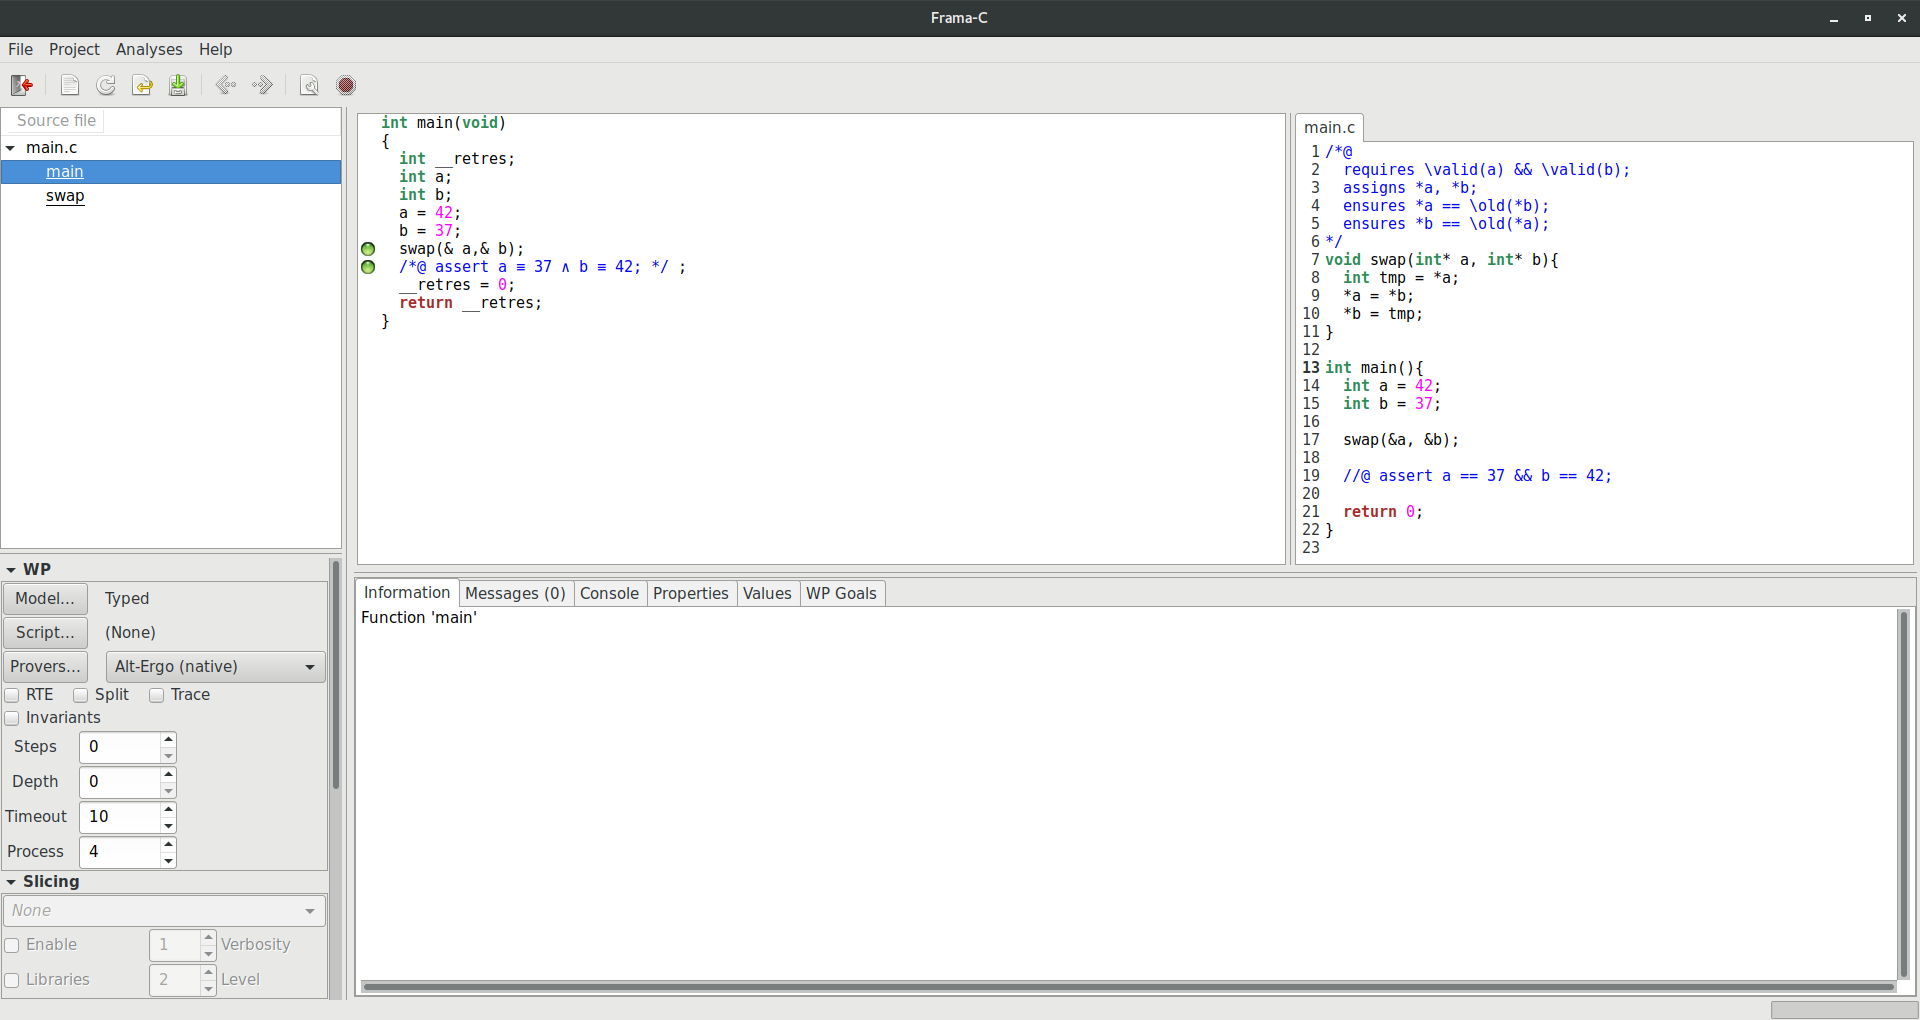
\includegraphics[scale=0.5]{1-2-verif_install-1.png}
\caption{Vérification installation 1}
\end{figure}

En cliquant sur \texttt{main.c} dans le volet latéral gauche pour le
sélectionner, vous devriez voir le contenu du fichier \texttt{main.c}
modifié et des pastilles vertes sur différentes lignes comme ceci :

\begin{figure}[htbp]
\centering
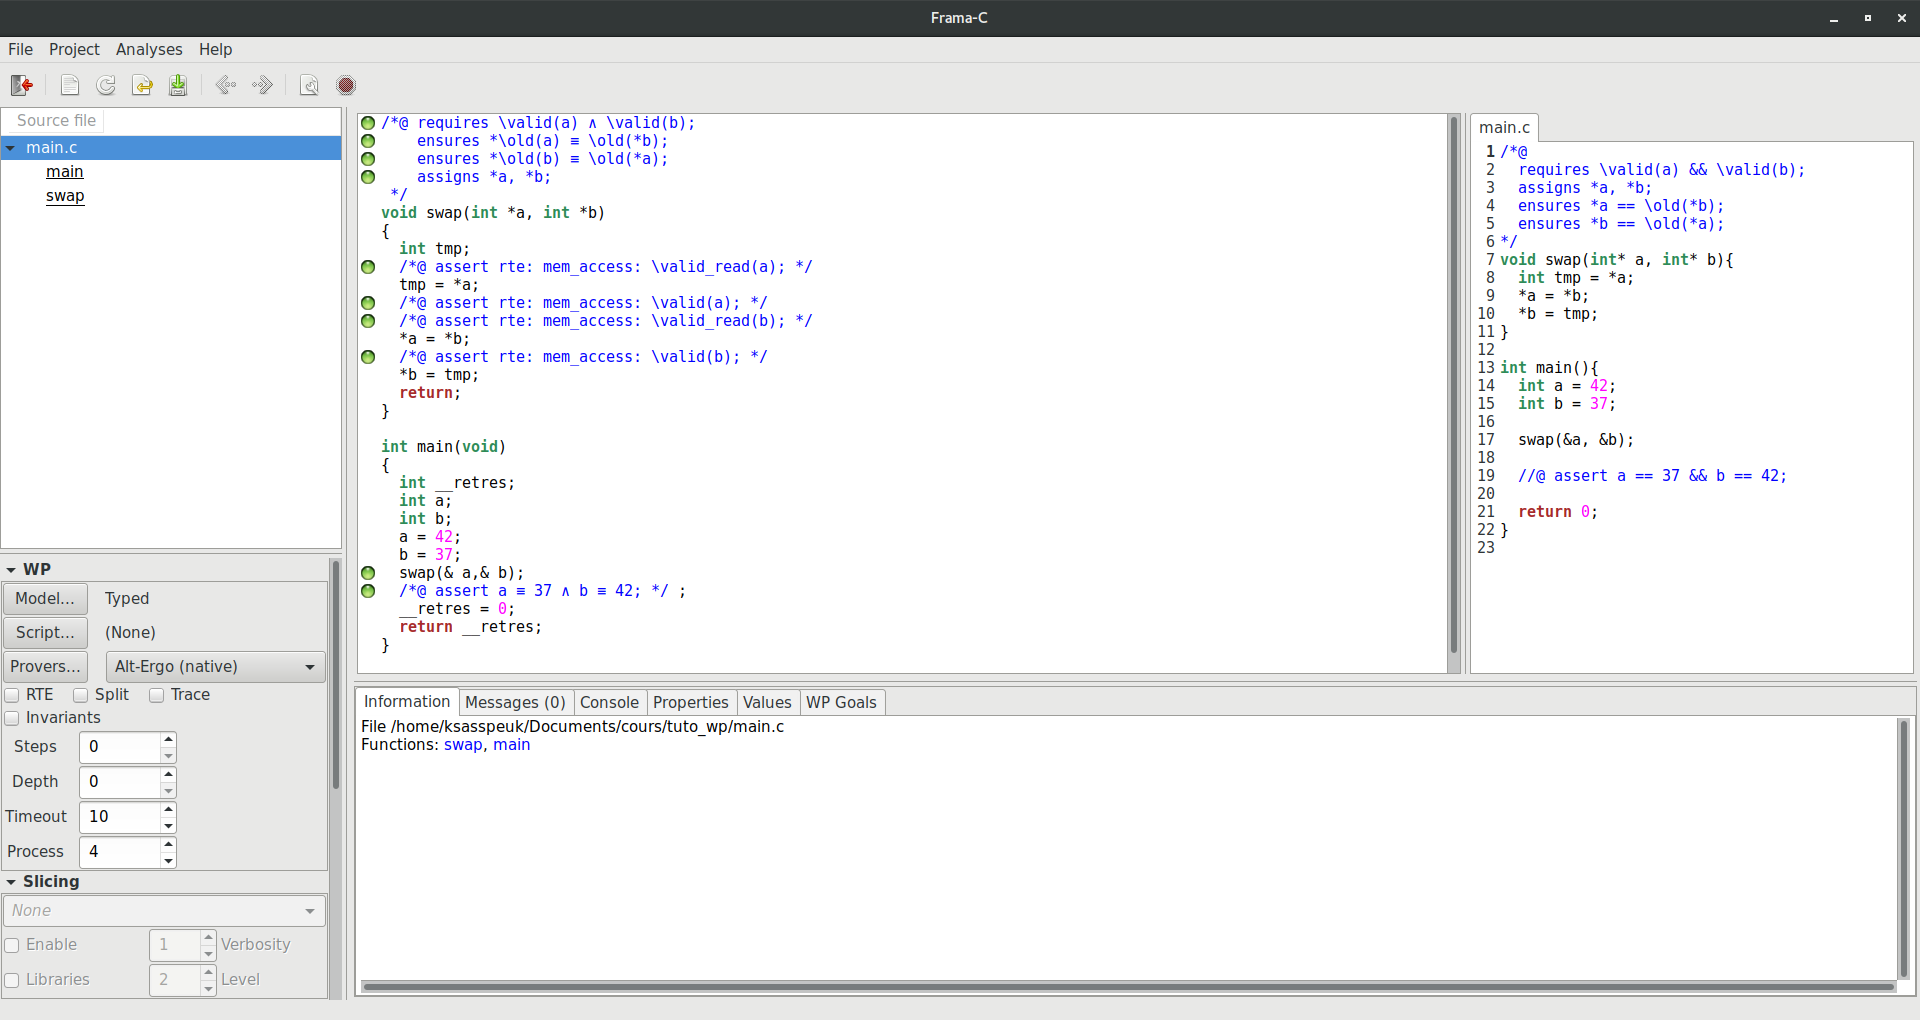
\includegraphics[scale=0.5]{1-2-verif_install-2.png}
\caption{Vérification installation 2}
\end{figure}

Si c'est le cas, tant mieux, sinon vérifiez d'abord que vous n'avez rien
raté de l'installation (par exemple : l'oubli de bibliothèques
graphiques ou encore l'oubli de l'installation d'Alt-Ergo). Si tout vous
semble bon, vous pouvez demander de l'aide sur divers forums.

\subsection{(Bonus) Installation de prouveurs
supplémentaires}\label{bonus-installation-de-prouveurs-suppluxe9mentaires}

Cette partie est purement optionnelle, rien de ce qui est ici ne vous
sera complètement nécessaire pendant le tutoriel. Cependant, si vous
commencez à vous intéresser vraiment à la preuve, il est possible que
vous touchiez à un moment ou un autre les limites du prouveur
pré-intégré Alt-Ergo et que vous ayez besoin d'outil plus puissants.

\subsubsection{Coq}\label{coq}

Coq, développé par l'organisme de recherche Inria, est un assistant de
preuve. C'est-à-dire que vous écrivez vous-même les preuves dans un
langage dédié et la plateforme se charge de vérifier (par typage) que
cette preuve est valide.

Pourquoi aurait-on besoin d'un tel outil ? Il se peut parfois que les
propriétés que vous voulez prouver soit trop complexe pour un prouveur
automatique, typiquement lorsqu'elles nécessitent des raisonnements par
induction avec des choix minutieux à chaque étape. Auquel cas, WP pourra
générer des obligations de preuve traduites en Coq et vous laisser
écrire la preuve en question.

Si vous voulez apprendre à utiliser Coq,
\href{http://www.cis.upenn.edu/~bcpierce/sf/current/index.html}{ce
tutoriel} est très bon.

\begin{zdsblock}{Information}
Si vous installez Frama-C par
l'intermédiaire de votre gestionnaire de paquets, il peut
arriver que celui-ci aie directement intégré Coq.

Pour plus d'informations à propos de Coq et de son installation, voir
par ici : \href{https://coq.inria.fr/}{The Coq Proof Assistant}.

Pour utiliser Coq lors d'une preuve dans Frama-C, il faudra le
sélectionner par l'intermédiaire du paneau latéral à gauche, dans la
partie qui concerne WP.
\end{zdsblock}

\begin{figure}[htbp]
\centering
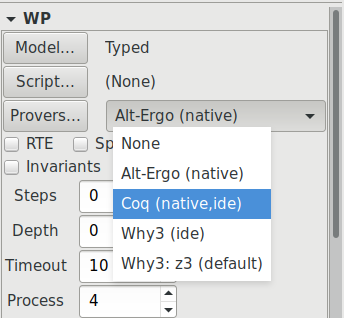
\includegraphics[scale=0.5]{1-2-select-coq.png}
\caption{Sélectionner l'assistant de preuve Coq}
\end{figure}

\begin{zdsblock}{Information}
  Je ne sais absolument pas si cette procédure est suffisante pour Windows.
\end{zdsblock}

\subsubsection{Why3}\label{why3}

\begin{zdsalertblock}{Attention}
  À ma connaissance, il n'est pas
  possible (ou vraiment pas facile) d'installer Why3 sous
  Windows. L'auteur ne saurait être tenu responsable de
  blessures que vous pourriez subir pendant une telle
  opération.
\end{zdsalertblock}

Why3 est une plateforme pour la preuve déductive développée par le LRI à
Orsay. Elle embarque en outre un langage de programmation et de
spécification ainsi qu'un module permettant le dialogue avec une large
variété de prouveurs automatiques et interactifs. C'est en cela qu'il
peut nous intéresser. WP sera capable de traduire ses obligations de
preuve vers le langage de Why3 et d'utiliser ce dernier pour dialoguer
avec un certain nombre de prouveurs automatiques.

Pour plus d'informations sur Why3 c'est \href{http://why3.lri.fr/}{sur
son site} que ça se passe. Si vous avez installé Opam, Why3 est
disponible par son intermédiaire. Sinon, vous pouvez aller voir la
procédure d'installation proposée.

Vous pouvez retrouver sur ce même site
\href{http://why3.lri.fr/\#provers}{la liste des prouveurs} qu'il
supporte. Il est vivement conseillé d'avoir
\href{https://github.com/Z3Prover/z3/wiki}{Z3}, développé par Microsoft
Research, et \href{http://cvc4.cs.nyu.edu/web/}{CVC4}, développé par des
personnes de divers organisme de recherche (New York University,
University of Iowa, Google, CEA LIST). Ces deux prouveurs sont très
efficaces et relativement complémentaires.

Pour utiliser les prouveurs en question, référez-vous à la partie sur
Coq pour la sélection d'un prouveur différent d'Alt-Ergo. À noter qu'il
faudra peut-être que vous demandiez la détection des prouveurs
fraîchement installé avec le bouton \og{}Provers\fg{} puis \og{}Detect Provers\fg{}
dans la fenêtre qui s'ouvre.

Voilà. Nos outils sont installés et prêts à fonctionner.

Le but de cette partie, en plus de l'installation de nos outils de
travail pour la suite, est de faire ressortir deux informations claires
:

\begin{itemize}
\tightlist
\item
  la preuve est un moyen d'assurer que nos programmes n'ont que des
  comportements conformes à notre spécification ;
\item
  il est toujours de notre devoir d'assurer que cette spécification est
  correcte.
\end{itemize}

\chapter{Contrats de fonctions}\label{contrats-de-fonctions}

Il est plus que temps d'entamer les hostilités. Contrairement aux
tutoriels sur divers langages, nous allons commencer par les fonctions.
D'abord parce qu'il faut savoir en écrire avant d'entamer un tel
tutoriel et surtout parce que cela permettra rapidement d'écrire
quelques preuves jouables.

Au contraire, après le travail sur les fonctions, nous entamerons les
notions les plus simples comme les affectations ou les structures
conditionnelles pour comprendre comment fonctionne l'outil sous le
capot.

Pour pouvoir prouver qu'un code est valide, il faut d'abord pouvoir
spécifier ce que nous attendons de lui. La preuve de programme
consistera donc à s'assurer que le code que nous avons écrit correspond
bien à la spécification qui décrit le rôle qui lui a été attribué. Comme
mentionné plus tôt dans le tutoriel, la spécification de code pour
Frama-C est faite avec le langage ACSL, celui-ci nous permet (mais pas
seulement, comme nous le verrons dans la suite) de poser un contrat pour
chaque fonction.

\section{Définition d'un contrat}\label{duxe9finition-dun-contrat}

Le principe d'un contrat de fonction est de poser les conditions selon
lesquelles la fonction va s'exécuter. C'est-à-dire ce que doit respecter
l'appelant pour que la fonction s'exécute correctement : la
pré-condition, la notion de \og{}s'exécute correctement\fg{} étant elle-même
définie dans le contrat par la post-condition.

Ces propriétés sont exprimées en langage ACSL, la syntaxe est
relativement simple pour qui a déjà fait du C puisqu'elle reprend la
syntaxe des expressions booléennes du C. Cependant, elle ajoute
également :

\begin{itemize}
\tightlist
\item
  certaines constructions et connecteurs logiques qui ne sont pas
  présents originellement en C pour faciliter l'écriture ;
\item
  des prédicats pré-implémentés pour exprimer des propriétés souvent
  utiles en C (par exemple : pointeur valide) ;
\item
  ainsi que des types plus généraux que les types primitifs du C,
  typiquement les types entiers ou réels.
\end{itemize}

Nous introduirons au fil du tutoriel les notations présentes dans le
langage ACSL.

Les spécifications ACSL sont introduites dans nos codes source par
l'intermédiaire d'annotations. Syntaxiquement, un contrat de fonction
est intégré dans les sources de la manière suivante :

\begin{footnotesize}\begin{Shaded}
\begin{Highlighting}[]
\CommentTok{/*@}
\CommentTok{  //contrat}
\CommentTok{*/}
\DataTypeTok{void} \NormalTok{foo(}\DataTypeTok{int} \NormalTok{bar)\{}

\NormalTok{\}}
\end{Highlighting}
\end{Shaded}\end{footnotesize}

Notons bien le \texttt{@} à la suite du début du bloc de commentaire,
c'est lui qui fait que ce bloc devient un bloc d'annotations pour
Frama-C et pas un simple bloc de commentaires à ignorer.

Maintenant, regardons comment sont exprimés les contrats.

\subsection{Post-condition}\label{post-condition}

La post-condition d'une fonction est précisée avec la clause
\texttt{ensures}. Nous allons travailler avec la fonction suivante qui
donne la valeur absolue. Un de ses post-conditions est que le résultat
(que nous notons avec le mot-clé \texttt{\textbackslash{}result}) est
supérieur ou égal à 0.

\begin{footnotesize}\begin{Shaded}
\begin{Highlighting}[]
\CommentTok{/*@}
\CommentTok{  ensures \textbackslash{}result >= 0;}
\CommentTok{*/}
\DataTypeTok{int} \NormalTok{abs(}\DataTypeTok{int} \NormalTok{val)\{}
  \KeywordTok{if}\NormalTok{(val < }\DecValTok{0}\NormalTok{) }\KeywordTok{return} \NormalTok{-val;}
  \KeywordTok{return} \NormalTok{val;}
\NormalTok{\}}
\end{Highlighting}
\end{Shaded}\end{footnotesize}

(Notons le \texttt{;} à la fin de la ligne de spécification comme en C).

Mais ce n'est pas tout, il faut également spécifier le comportement
général attendu d'une fonction renvoyant la valeur absolue. À savoir :
si la valeur est positive ou nulle, la fonction renvoie la même valeur,
sinon elle renvoie l'opposée de la valeur.

Nous pouvons spécifier plusieurs post-conditions, soit en les composants
avec un \texttt{\&\&} comme en C, soit en introduisant une nouvelle
clause \texttt{ensures}, comme illustré ci-dessous.

\begin{footnotesize}\begin{Shaded}
\begin{Highlighting}[]
\CommentTok{/*@}
\CommentTok{  ensures \textbackslash{}result >= 0;}
\CommentTok{  ensures (val >= 0 ==> \textbackslash{}result == val ) && }
\CommentTok{          (val <  0 ==> \textbackslash{}result == -val);}
\CommentTok{*/}
\DataTypeTok{int} \NormalTok{abs(}\DataTypeTok{int} \NormalTok{val)\{}
  \KeywordTok{if}\NormalTok{(val < }\DecValTok{0}\NormalTok{) }\KeywordTok{return} \NormalTok{-val;}
  \KeywordTok{return} \NormalTok{val;}
\NormalTok{\}}
\end{Highlighting}
\end{Shaded}\end{footnotesize}

Cette spécification est l'opportunité de présenter un connecteur logique
très utile que propose ACSL mais qui n'est pas présent en C :
l'implication \texttt{A\ ==\textgreater{}\ B}. La table de vérité de
l'implication est la suivante :

\begin{longtable}[]{@{}lll@{}}
\toprule
A & B & Resultat\tabularnewline
\midrule
\endhead
false & true & true\tabularnewline
false & false & true\tabularnewline
true & true & true\tabularnewline
true & false & false\tabularnewline
\bottomrule
\end{longtable}

Ce qui veut dire qu'une implication \texttt{A\ ==\textgreater{}\ B} est
vraie dans deux cas : soit A est fausse (et dans ce cas, il ne faut pas
se préoccuper de B), soit A est vraie et alors B doit être vraie aussi.
L'idée étant finalement \og{}je veux savoir si dans le cas où A est vrai, B
l'est aussi. Si A est faux, je considère que l'ensemble est vrai\fg{}.

Sa cousine l'équivalence \texttt{A\ \textless{}==\textgreater{}\ B} est
plus forte. C'est la conjonction de l'implication dans les deux sens :
\texttt{(A\ ==\textgreater{}\ B)\ \&\&\ (B\ ==\textgreater{}\ A)}. Cette
formule n'est vraie que dans deux cas : A et B sont vraies toutes les
deux, ou fausses toutes les deux (c'est donc la négation du
ou-exclusif).

Revenons à notre spécification. Quand nos fichiers commencent à être
longs et contenir beaucoup de spécifications, il peut être commode de
nommer les propriétés que nous souhaitons vérifier. Pour cela, nous
indiquons un nom (les espaces ne sont pas autorisées) suivi de
\texttt{:} avant de mettre effectivement la propriété, il est possible
de mettre plusieurs \og{}étages\fg{} de noms pour catégoriser nos propriétés.
Par exemple nous pouvons écrire ceci :

\begin{footnotesize}\begin{Shaded}
\begin{Highlighting}[]
\CommentTok{/*@}
\CommentTok{  ensures positive_value: function_result: \textbackslash{}result >= 0;}
\CommentTok{  ensures (val >= 0 ==> \textbackslash{}result == val) && }
\CommentTok{          (val < 0 ==> \textbackslash{}result == -val);}
\CommentTok{*/}
\DataTypeTok{int} \NormalTok{abs(}\DataTypeTok{int} \NormalTok{val)\{}
  \KeywordTok{if}\NormalTok{(val < }\DecValTok{0}\NormalTok{) }\KeywordTok{return} \NormalTok{-val;}
  \KeywordTok{return} \NormalTok{val;}
\NormalTok{\}}
\end{Highlighting}
\end{Shaded}\end{footnotesize}

Dans une large part du tutoriel, nous ne nommerons pas les éléments que
nous tenterons de prouver, les propriétés seront généralement
relativement simples et peu nombreuses, les noms n'apporteraient pas
beaucoup d'information.

Nous pouvons copier/coller la fonction \texttt{abs} et sa spécification
dans un fichier abs.c et regarder avec Frama-C si l'implémentation est
conforme à la spécification.

Pour cela, il faut lancer l'interface graphique de Frama-C (il est
également possible de se passer de l'interface graphique, cela ne sera
pas présenté dans ce tutoriel) soit par cette commande :

\begin{footnotesize}\begin{Shaded}
\begin{Highlighting}[]
\NormalTok{$ }\KeywordTok{frama-c-gui}
\end{Highlighting}
\end{Shaded}\end{footnotesize}

Soit en l'ouvrant depuis l'environnement graphique.

Il est ensuite possible de cliquer sur le bouton \og{}Create a new session
from existing C files\fg{}, les fichiers à analyser peuvent être
sélectionnés par double-clic, OK terminant la sélection. Par la suite,
l'ajout d'autres fichiers à la session s'effectue en cliquant sur Files
\textgreater{} Source Files.

À noter également qu'il est possible de directement ouvrir le(s)
fichier(s) depuis la ligne de commande en le(s) passant en argument(s)
de \texttt{frama-c-gui}.

\begin{footnotesize}\begin{Shaded}
\begin{Highlighting}[]
\NormalTok{$ }\KeywordTok{frama-c-gui} \NormalTok{abs.c}
\end{Highlighting}
\end{Shaded}\end{footnotesize}

\begin{figure}[htbp]
\centering
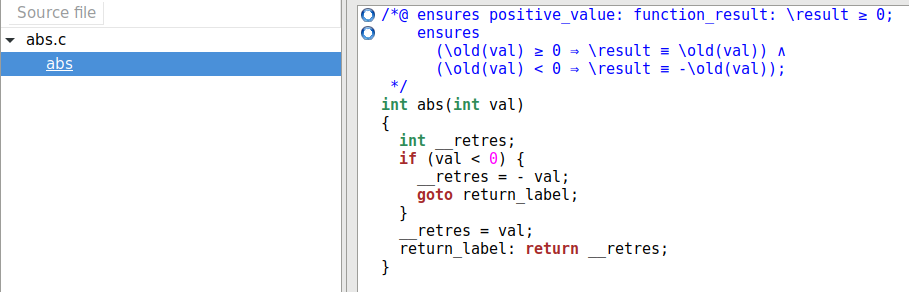
\includegraphics[scale=0.5]{2-1-1-abs-1.png}
\caption{Le volet latéral liste l'arbre des fichiers et des fonctions}
\end{figure}

La fenêtre de Frama-C s'ouvre, dans le volet correspondant aux fichiers
et aux fonctions, nous pouvons sélectionner la fonction \texttt{abs}.
Aux différentes lignes \texttt{ensures}, il y a un cercle bleu dans la
marge, ils indiquent qu'aucune vérification n'a été tentée pour ces
lignes.

Nous demandons la vérification que le code répond à la spécification en
faisant un clic droit sur le nom de la fonction et \og{}Prove function
annotations by WP\fg{} :

\begin{figure}[htbp]
\centering
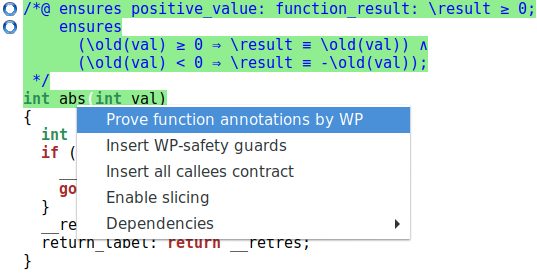
\includegraphics[scale=0.5]{2-1-1-abs-2.png}
\caption{Lancer la vérification de \texttt{abs} avec WP}
\end{figure}

Nous pouvons voir que les cercles bleus deviennent des pastilles vertes,
indiquant que la spécification est bien assurée par le programme. Il est
possible de prouver les propriétés une à une en cliquant droit sur
celles-ci et pas sur le nom de la fonction.

Mais le code est-il vraiment sans erreur pour autant ? WP nous permet de
nous assurer que le code répond à la spécification, mais il ne fait pas
de contrôle d'erreur à l'exécution (RunTime Error : RTE). C'est le rôle
d'un autre petit plugin que nous allons utiliser ici et qui s'appelle
sobrement RTE. Son but est d'ajouter des contrôles dans le programme
pour les erreurs d'exécutions possibles (débordements d'entiers,
déréférencements de pointeurs invalides, division par 0, etc).

Pour activer ce contrôle, nous cochons la case montrée par cette capture
(dans le volet de WP). Il est également possible de demander à Frama-C
d'ajouter ces contrôles par un clic droit sur le nom de la fonction puis
\og{}Insert RTE guards\fg{}.

\begin{figure}[htbp]
\centering
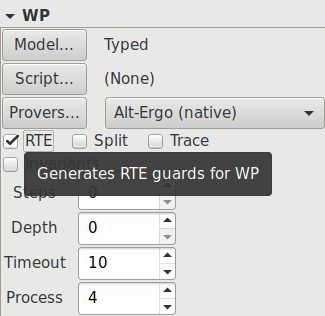
\includegraphics[scale=0.5]{2-1-1-abs-3.png}
\caption{Activer la vérification des erreurs d'exécution}
\end{figure}

Enfin nous relançons la vérification (nous pouvons également cliquer sur
le bouton \og{}Reparse\fg{} de la barre d'outils, cela aura pour effet de
supprimer les preuves déjà effectuées).

Nous pouvons alors voir alors que WP échoue à prouver l'impossibilité de
débordement arithmétique sur le calcul de -val. Et c'est bien normal
parce que -\texttt{INT\_MIN} (\(-2^{31}\)) \textgreater{}
\texttt{INT\_MAX} (\(2^{31}-1\)).

\begin{figure}[htbp]
\centering
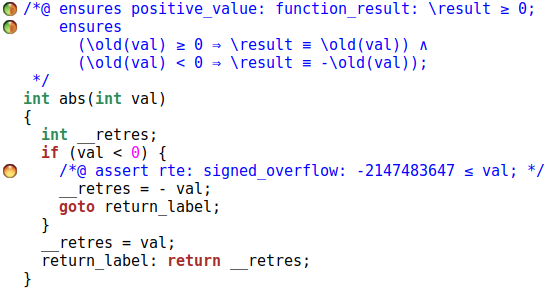
\includegraphics[scale=0.5]{2-1-1-abs-4.png}
\caption{Preuve incomplète de \texttt{abs}}
\end{figure}

Ici nous pouvons voir un autre type d'annotation ACSL. La ligne
\texttt{//@\ assert\ propriete\ ;} nous permet de demander la
vérification d'une propriété à un point particulier de programme. Ici,
l'outil l'a insérée pour nous car il faut vérifier que le \texttt{-val}
ne provoque pas de débordement, mais il est également possible d'en
ajouter manuellement dans un code.

Comme le montre cette capture d'écran, nous avons deux nouveaux codes
couleur pour les pastilles : vert+marron et orange.

La couleur vert + marron nous indique que la preuve a été effectué mais
qu'elle dépend potentiellement de propriétés qui, elle, ne l'ont pas
été. Si la preuve n'est pas recommencée intégralement par rapport à la
preuve précédente, ces pastilles ont dû rester vertes car les preuves
associées ont été réalisées avant l'introduction de la propriété nous
assurant l'absence de runtime-error, et ne se sont donc pas reposées sur
la connaissance de cette propriété puisqu'elle n'existait pas.

La couleur orange nous signale qu'aucun prouveur n'a pu déterminer si la
propriété est vérifiable. Les deux raisons peuvent être :

\begin{itemize}
\tightlist
\item
  qu'il n'a pas assez d'information pour le déterminer ;
\item
  que malgré toutes ses recherches, il n'a pas pu trouver un résultat à
  temps. Auquel cas, il rencontre un timeout dont la durée est
  configurable dans le volet de WP.
\end{itemize}

Dans le volet inférieur, nous pouvons sélectionner l'onglet \og{}WP
Goals\fg{}, celui-ci nous affiche la liste des obligations de preuve et
pour chaque prouveur indique un petit logo si la preuve a été tentée et
si elle a été réussie, échouée ou a rencontré un timeout (ici nous
pouvons voir un essai avec Z3 sur le contrôle de la RTE pour montrer le
logo des ciseaux associé au timeout).

\begin{figure}[htbp]
\centering
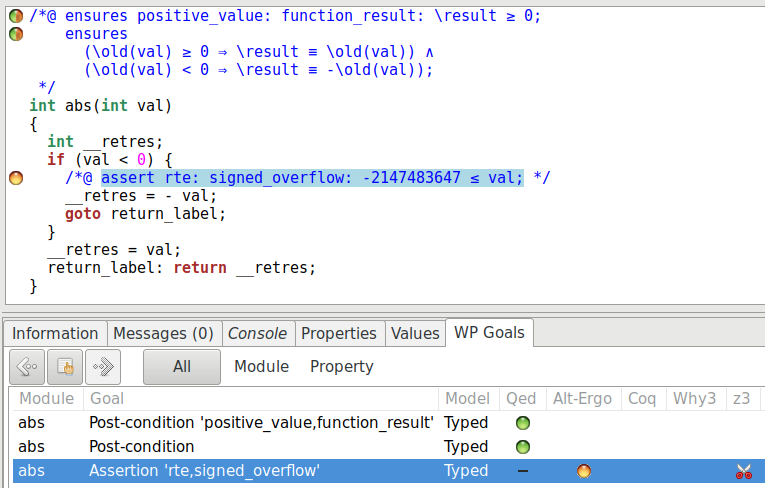
\includegraphics[scale=0.5]{2-1-1-abs-5.png}
\caption{Tableau des obligations de preuve de WP pour \texttt{abs}}
\end{figure}

Le tableau est découpé comme suit, en première colonne nous avons le nom
de la fonction où se trouve le but à prouver. En seconde colonne nous
trouvons le nom du but. Ici par exemple notre post-condition nommée est
estampillée \og{}Post-condition `positive\_value,function\_result'\,\fg{},
nous pouvons d'ailleurs noter que lorsqu'une propriété est sélectionnée
dans le tableau, elle est également sur-lignée dans le code source. Les
propriétés non-nommées se voient assignées comme nom le type de
propriété voulu. En troisième colonne, nous trouvons le modèle mémoire
utilisé pour la preuve, (nous n'en parlerons pas dans ce tutoriel).
Finalement, les dernières colonnes représentent les différents prouveurs
accessibles à WP.

Dans ces prouveurs, le premier élément de la colonne est Qed. Ce n'est
pas à proprement parler un prouveur. En fait, si nous double-cliquons
sur la propriété \og{}ne pas déborder\fg{} (surlignée en bleu dans la capture
précédente), nous pouvons voir ceci :

\begin{figure}[htbp]
\centering
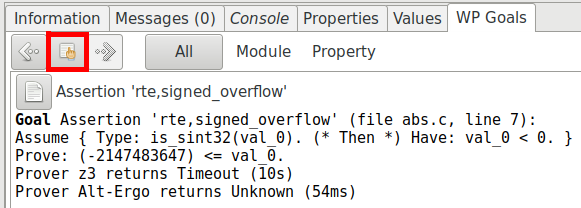
\includegraphics[scale=0.5]{2-1-1-abs-6.png}
\caption{Obligation de preuve associée à la vérification de débordement
dans \texttt{abs}}
\end{figure}

C'est l'obligation de preuve que génère WP par rapport à notre propriété
et notre programme, il n'est pas nécessaire de comprendre tout ce qui
s'y passe, juste d'avoir une idée globale. Elle contient (dans la partie
\og{}Assume\fg{}) les suppositions que nous avons pu donner et celles que WP a
pu déduire des instructions du programme. Elle contient également (dans
la partie \og{}Prove\fg{}) la propriété que nous souhaitons vérifier.

Que fait WP avec ces éléments ? En fait, il les transforme en une
formule logique puis demande aux différents prouveurs s'il est possible
de la satisfaire (de trouver pour chaque variable, une valeur qui rend
la formule vraie), cela détermine si la propriété est prouvable. Mais
avant d'envoyer cette formule aux prouveurs, WP utilise un module qui
s'appelle Qed et qui est capable de faire différentes simplifications à
son sujet. Parfois comme dans le cas des autres propriétés de
\texttt{abs}, ces simplifications suffisent à déterminer que la
propriété est forcément vraie, auquel cas, nous ne faisons pas appel aux
prouveurs.

Lorsque les prouveurs automatiques ne parviennent pas à assurer que nos
propriétés sont bien vérifiées, il est parfois difficile de comprendre
pourquoi. En effet, les prouveurs ne sont généralement pas capables de
nous répondre autre chose que \og{}oui\fg{}, \og{}non\fg{} ou \og{}inconnu\fg{}, ils ne
sont pas capables d'extraire le \og{}pourquoi\fg{} d'un \og{}non\fg{} ou d'un
\og{}inconnu\fg{}. Il existe des outils qui sont capables d'explorer les
arbres de preuve pour en extraire ce type d'information, Frama-C n'en
possède pas à l'heure actuelle. La lecture des obligations de preuve
peut parfois nous aider, mais cela demande un peu d'habitude pour
pouvoir les déchiffrer facilement. Finalement, le meilleur moyen de
comprendre la raison d'un échec est d'effectuer la preuve de manière
interactive avec Coq. En revanche, il faut déjà avoir une certaine
habitude de ce langage pour ne pas être perdu devant les obligations de
preuve générées par WP, étant donné que celles-ci encodent les éléments
de la sémantique de C, ce qui rend le code souvent indigeste.

Si nous retournons dans notre tableau des obligations de preuve (bouton
encadré dans la capture d'écran précédente), nous pouvons donc voir que
les hypothèses n'ont pas suffi aux prouveurs pour déterminer que la
propriété est vraie (et nous l'avons dit : c'est normal), il nous faut
donc ajouter une hypothèse supplémentaire pour garantir le bon
fonctionnement de la fonction : une pré-condition d'appel.

\subsection{Pré-condition}\label{pruxe9-condition}

Les pré-conditions de fonctions sont introduites par la clause
\texttt{requires}, de la même manière qu'avec \texttt{ensures}, nous
pouvons composer nos expressions logiques et mettre plusieurs
pré-condition :

\begin{footnotesize}\begin{Shaded}
\begin{Highlighting}[]
\CommentTok{/*@}
\CommentTok{  requires 0 <= a < 100;}
\CommentTok{  requires b < a;}
\CommentTok{*/}
\DataTypeTok{void} \NormalTok{foo(}\DataTypeTok{int} \NormalTok{a, }\DataTypeTok{int} \NormalTok{b)\{}
  
\NormalTok{\}}
\end{Highlighting}
\end{Shaded}\end{footnotesize}

Les pré-conditions sont des propriétés sur les entrées (et
potentiellement sur des variables globales) qui seront supposées
préalablement vraies lors de l'analyse de la fonction. La preuve que
celles-ci sont effectivement validées n'interviendra qu'aux points où la
fonction est appelée.

Dans ce petit exemple, nous pouvons également noter une petite
différence avec C dans l'écriture des expressions booléennes. Si nous
voulons spécifier que \texttt{a} se trouve entre 0 et 100, il n'y a pas
besoin d'écrire \texttt{0\ \textless{}=\ a\ \&\&\ a\ \textless{}\ 100}
(c'est-à-dire en composant les deux comparaisons avec un \texttt{\&\&}).
Nous pouvons simplement écrire
\texttt{0\ \textless{}=\ a\ \textless{}\ 100} et l'outil se chargera de
faire la traduction nécessaire.

Si nous revenons à notre exemple de la valeur absolue, pour éviter le
débordement arithmétique, il suffit que la valeur de val soit
strictement supérieure à \texttt{INT\_MIN} pour garantir que le
débordement n'arrivera pas. Nous l'ajoutons donc comme pré-condition (à
noter : il faut également inclure le header où \texttt{INT\_MIN} est
défini) :

\begin{footnotesize}\begin{Shaded}
\begin{Highlighting}[]
\CommentTok{#include <limits.h>}

\CommentTok{/*@}
\CommentTok{  requires INT_MIN < val;}

\CommentTok{  ensures \textbackslash{}result >= 0;}
\CommentTok{  ensures (val >= 0 ==> \textbackslash{}result == val) && }
\CommentTok{          (val < 0 ==> \textbackslash{}result == -val);}
\CommentTok{*/}
\DataTypeTok{int} \NormalTok{abs(}\DataTypeTok{int} \NormalTok{val)\{}
  \KeywordTok{if}\NormalTok{(val < }\DecValTok{0}\NormalTok{) }\KeywordTok{return} \NormalTok{-val;}
  \KeywordTok{return} \NormalTok{val;}
\NormalTok{\}}
\end{Highlighting}
\end{Shaded}\end{footnotesize}

\begin{zdsalertblock}{Attention}
  La fenêtre de Frama-C ne permet pas
  l'édition du code source.
\end{zdsalertblock}

Une fois le code source modifié de cette manière, un clic sur
\og{}Reparse\fg{} et nous lançons à nouveau l'analyse. Cette fois, tout est
validé pour WP, notre implémentation est prouvée :

\begin{figure}[htbp]
\centering
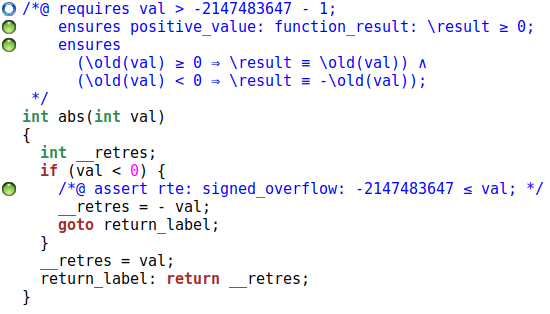
\includegraphics[scale=0.5]{2-1-2-abs-1.png}
\caption{Preuve de \texttt{abs} effectuée}
\end{figure}

Nous pouvons également vérifier qu'une fonction qui appellerait
\texttt{abs} respecte bien la pré-condition qu'elle impose :

\begin{footnotesize}\begin{Shaded}
\begin{Highlighting}[]
\DataTypeTok{void} \NormalTok{foo(}\DataTypeTok{int} \NormalTok{a)\{}
   \DataTypeTok{int} \NormalTok{b = abs(}\DecValTok{42}\NormalTok{);}
   \DataTypeTok{int} \NormalTok{c = abs(-}\DecValTok{42}\NormalTok{);}
   \DataTypeTok{int} \NormalTok{d = abs(a);       }\CommentTok{// Faux : "a", vaut peut être INT_MIN}
   \DataTypeTok{int} \NormalTok{e = abs(INT_MIN); }\CommentTok{// Faux : le paramètre doit être strictement supérieur à INT_MIN}
\NormalTok{\}}
\end{Highlighting}
\end{Shaded}\end{footnotesize}

\begin{figure}[htbp]
\centering
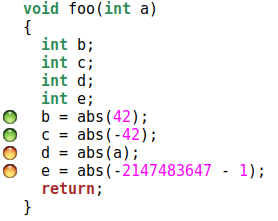
\includegraphics[scale=0.5]{2-1-2-foo-1.png}
\caption{Vérification du contrat à l'appel de \texttt{abs}}
\end{figure}

Pour modifier un peu l'exemple, nous pouvons essayer d'inverser les deux
dernières lignes. Auquel cas, nous pouvons voir que l'appel
\texttt{abs(a)} est validé par WP s'il se trouve après l'appel
\texttt{abs(INT\_MIN)} ! Pourquoi ?

Il faut bien garder en tête que le principe de la preuve déductive est
de nous assurer que si les pré-conditions sont vérifiées et que le
calcul termine alors la post-condition est vérifiée.

Si nous donnons à notre fonction une valeur qui viole ses
pré-conditions, alors nous en déduisons que la post-condition est
fausse. À partir de là, nous pouvons prouver tout ce que nous voulons
car ce \og{}false\fg{} devient une pré-condition pour tout appel qui viendrait
ensuite. À partir de faux, nous prouvons tout ce que nous voulons, car
si nous avons la preuve de \og{}faux\fg{} alors \og{}faux\fg{} est vrai, de même que
\og{}vrai\fg{} est vrai. Donc tout est vrai.

En prenant le programme modifié, nous pouvons d'ailleurs regarder les
obligations de preuve générées par WP pour l'appel fautif et l'appel
prouvé par conséquent :

\begin{figure}[htbp]
\centering
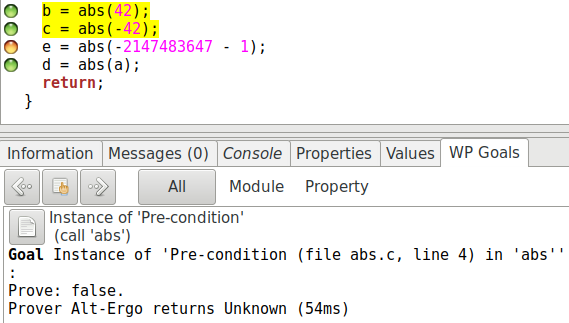
\includegraphics[scale=0.5]{2-1-2-foo-2.png}
\caption{Obligation générée pour l'appel fautif}
\end{figure}

\begin{figure}[htbp]
\centering
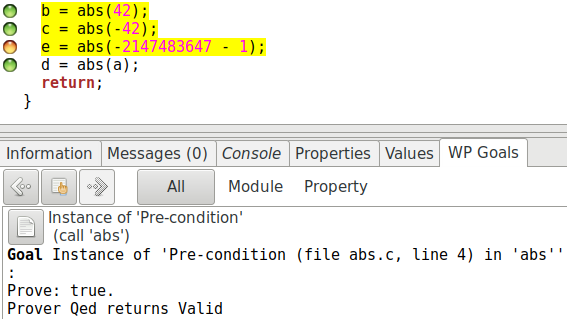
\includegraphics[scale=0.5]{2-1-2-foo-3.png}
\caption{Obligation générée pour l'appel qui suit}
\end{figure}

Nous pouvons remarquer que pour les appels de fonctions, l'interface
graphique nous surligne le chemin d'exécution suivi avant l'appel dont
nous cherchons à vérifier la pré-condition. Ensuite, si nous regardons
l'appel \texttt{abs(INT\_MIN)}, nous pouvons remarquer qu'à force de
simplifications, Qed a déduit que nous cherchons à prouver \og{}False\fg{}.
Conséquence logique, l'appel suivant \texttt{abs(a)} reçoit dans ses
suppositions \og{}False\fg{}. C'est pourquoi Qed est capable de déduire
immédiatement \og{}True\fg{}.

La deuxième partie de la question est alors : pourquoi lorsque nous
mettons les appels dans l'autre sens (\texttt{abs(a)} puis
\texttt{abs(INT\_MIN)}), nous obtenons quand même une violation de la
pré-condition sur le deuxième ? La réponse est simplement que
\texttt{abs(a)} peut, ou ne peut pas, provoquer une erreur, alors que
\texttt{abs(INT\_MIN)} provoque forcément l'erreur. Dans le premier cas,
nous apprenons nécessairement \og{}faux\fg{}, pas dans le deuxième cas.

Bien spécifier son programme est donc d'une importance cruciale.
Typiquement, préciser un pré-condition fausse peut nous donner la
possibilité de prouver FAUX :

\begin{footnotesize}\begin{Shaded}
\begin{Highlighting}[]
\CommentTok{/*@}
\CommentTok{  requires a < 0 && a > 0;}
\CommentTok{  ensures  \textbackslash{}false;}
\CommentTok{*/}
\DataTypeTok{void} \NormalTok{foo(}\DataTypeTok{int} \NormalTok{a)\{}

\NormalTok{\}}
\end{Highlighting}
\end{Shaded}\end{footnotesize}

Si nous demandons à WP de prouver cette fonction. Il l'acceptera sans
rechigner car la supposition que nous lui donnons en entrée est
nécessairement fausse. Par contre, nous aurons bien du mal à lui donner
une valeur en entrée qui respecte la pré-condition, nous pourrons donc
nous en apercevoir.

Certaines notions que nous verrons plus loin dans le tutoriel
apporterons un risque encore plus grand de créer ce genre d'incohérence.
Il faut donc toujours avoir une attention particulière pour ce que nous
spécifions.

\subsection{Quelques éléments sur l'usage de WP et
Frama-C}\label{quelques-uxe9luxe9ments-sur-lusage-de-wp-et-frama-c}

Dans les deux sous-sections précédentes, nous avons vu maximum
d'éléments à propos de l'usage de la GUI pour lancer les preuves. En
fait, il est possible de demander immédiatement à WP d'effectuer les
preuves pendant le lancement de Frama-C avec la commande :

\begin{footnotesize}\begin{Shaded}
\begin{Highlighting}[]
\NormalTok{$ }\KeywordTok{frama-c-gui} \NormalTok{file.c -wp}
\end{Highlighting}
\end{Shaded}\end{footnotesize}

Cela demande à WP d'immédiatement faire les calculs de plus faible
pré-condition et de lancer les prouveurs les buts générés.

Concernant les contrôles des RTE, il est généralement conseillé de
commencer par vérifier le programme sans mettre les contrôles de RTE. Et
ensuite seulement de générer les assertions correspondantes pour
terminer la vérification avec WP. Cela permet à WP de se \og{}concentrer\fg{}
dans un premier temps sur les propriétés fonctionnelles sans avoir la
connaissance de propriétés purement techniques dues à C, qui chargent
inutilement la base de connaissances. Une nouvelle fois, il est possible
de produire ce comportement directement depuis la ligne de commande en
écrivant :

\begin{footnotesize}\begin{Shaded}
\begin{Highlighting}[]
\NormalTok{$ }\KeywordTok{frama-c-gui} \NormalTok{file.c -wp -then -rte -wp}
\end{Highlighting}
\end{Shaded}\end{footnotesize}

\og{}Lancer Frama-C avec WP, puis créer les assertions correspondant aux
RTE, et lancer à nouveau WP\fg{}.

\section{De l'importance d'une bonne
spécification}\label{de-limportance-dune-bonne-spuxe9cification}

\subsection{Bien traduire ce qui est
attendu}\label{bien-traduire-ce-qui-est-attendu}

C'est certainement notre tâche la plus difficile. En soi, la
programmation est déjà un effort consistant à écrire des algorithmes qui
répondent à notre besoin. La spécification nous demande également de
faire ce travail, la différence est que nous ne nous occupons plus de
préciser la manière de répondre au besoin mais le besoin lui-même. Pour
prouver que la réalisation implémente bien ce que nous attendons, il
faut donc être capable de décrire précisément le besoin.

Changeons d'exemple et spécifions la fonction suivante :

\begin{footnotesize}\begin{Shaded}
\begin{Highlighting}[]
\DataTypeTok{int} \NormalTok{max(}\DataTypeTok{int} \NormalTok{a, }\DataTypeTok{int} \NormalTok{b)\{}
  \KeywordTok{return} \NormalTok{(a > b) ? a : b;}
\NormalTok{\}}
\end{Highlighting}
\end{Shaded}\end{footnotesize}

Le lecteur pourra écrire et prouver sa spécification. Pour la suite,
nous travaillerons avec celle-ci :

\begin{footnotesize}\begin{Shaded}
\begin{Highlighting}[]
\CommentTok{/*@}
\CommentTok{  ensures \textbackslash{}result >= a && \textbackslash{}result >= b;}
\CommentTok{*/}
\DataTypeTok{int} \NormalTok{max(}\DataTypeTok{int} \NormalTok{a, }\DataTypeTok{int} \NormalTok{b)\{}
  \KeywordTok{return} \NormalTok{(a > b) ? a : b;}
\NormalTok{\}}
\end{Highlighting}
\end{Shaded}\end{footnotesize}

Si nous donnons ce code à WP, il accepte sans problème de prouver la
fonction. Pour autant cette spécification est-elle juste ? Nous pouvons
par exemple essayer de voir si ce code est validé :

\begin{footnotesize}\begin{Shaded}
\begin{Highlighting}[]
\DataTypeTok{void} \NormalTok{foo()\{}
  \DataTypeTok{int} \NormalTok{a = }\DecValTok{42}\NormalTok{;}
  \DataTypeTok{int} \NormalTok{b = }\DecValTok{37}\NormalTok{;}
  \DataTypeTok{int} \NormalTok{c = max(a,b);}

  \CommentTok{//@assert c == 42;}
\NormalTok{\}}
\end{Highlighting}
\end{Shaded}\end{footnotesize}

La réponse est non. En fait, nous pouvons aller plus loin en modifiant
le corps de la fonction \texttt{max} et remarquer que le code suivant
est également valide quant à la spécification :

\begin{footnotesize}\begin{Shaded}
\begin{Highlighting}[]
\CommentTok{#include <limits.h>}

\CommentTok{/*@}
\CommentTok{  ensures \textbackslash{}result >= a && \textbackslash{}result >= b;}
\CommentTok{*/}
\DataTypeTok{int} \NormalTok{max(}\DataTypeTok{int} \NormalTok{a, }\DataTypeTok{int} \NormalTok{b)\{}
  \KeywordTok{return} \NormalTok{INT_MAX;}
\NormalTok{\}}
\end{Highlighting}
\end{Shaded}\end{footnotesize}

Notre spécification est trop permissive. Il faut que nous soyons plus
précis. Nous attendons du résultat non seulement qu'il soit supérieur ou
égal à nos deux paramètres mais également qu'il soit exactement l'un des
deux :

\begin{footnotesize}\begin{Shaded}
\begin{Highlighting}[]
\CommentTok{/*@}
\CommentTok{  ensures \textbackslash{}result >= a && \textbackslash{}result >= b;}
\CommentTok{  ensures \textbackslash{}result == a || \textbackslash{}result == b;}
\CommentTok{*/}
\DataTypeTok{int} \NormalTok{max(}\DataTypeTok{int} \NormalTok{a, }\DataTypeTok{int} \NormalTok{b)\{}
  \KeywordTok{return} \NormalTok{(a > b) ? a : b;}
\NormalTok{\}}
\end{Highlighting}
\end{Shaded}\end{footnotesize}

\subsection{Pointeurs}\label{pointeurs}

S'il y a une notion à laquelle nous sommes confrontés en permanence en
langage C, c'est bien la notion de pointeur. C'est une notion complexe
et l'une des principales cause de bugs critiques dans les programmes,
ils ont donc droit à un traitement de faveur dans ACSL.

Prenons par exemple une fonction swap pour les entiers :

\begin{footnotesize}\begin{Shaded}
\begin{Highlighting}[]
\CommentTok{/*@}
\CommentTok{  ensures *a == \textbackslash{}old(*b) && *b == \textbackslash{}old(*a);}
\CommentTok{*/}
\DataTypeTok{void} \NormalTok{swap(}\DataTypeTok{int}\NormalTok{* a, }\DataTypeTok{int}\NormalTok{* b)\{}
  \DataTypeTok{int} \NormalTok{tmp = *a;}
  \NormalTok{*a = *b;}
  \NormalTok{*b = tmp;}
\NormalTok{\}}
\end{Highlighting}
\end{Shaded}\end{footnotesize}

\subsubsection{Historique des valeurs}\label{historique-des-valeurs}

Ici, j'ai introduit une première fonction logique fournie de base par
ACSL : \texttt{\textbackslash{}old}, qui permet de parler de l'ancienne
valeur d'un élément. Ce que nous dit donc la spécification c'est \og{}la
fonction doit assurer que a soit égal à l'ancienne valeur (au sens : la
valeur avant l'appel) de b et inversement\fg{}.

La fonction \texttt{\textbackslash{}old} ne peut être utilisée que dans
la post-condition d'une fonction. Si nous avons besoin de ce type
d'information ailleurs, nous utilisons \texttt{\textbackslash{}at} qui
nous permet de statuer à propos de la valeur d'une variable à un point
donné. Elle reçoit deux paramètres. Le premier est la variable (ou
position mémoire) dont nous voulons obtenir la valeur et le second la
position (sous la forme d'un label C) à laquelle nous voulons contrôler
la valeur en question.

Par exemple, nous pourrions écrire :

\begin{footnotesize}\begin{Shaded}
\begin{Highlighting}[]
  \DataTypeTok{int} \NormalTok{a = }\DecValTok{42}\NormalTok{;}
 \NormalTok{Label_a:}
  \NormalTok{a = }\DecValTok{45}\NormalTok{;}

  \CommentTok{//@assert a == 45 && \textbackslash{}at(a, Label_a) == 42;}
\end{Highlighting}
\end{Shaded}\end{footnotesize}

En plus des labels que nous pouvons nous-mêmes créer. Il existe 6 labels
qu'ACSL nous propose par défaut, mais tous ne sont pas supportés par WP
:

\begin{itemize}
\tightlist
\item
  \texttt{Pre}/\texttt{Old} : valeur avant l'appel de la fonction,
\item
  \texttt{Post} : valeur après l'appel de la fonction,
\item
  \texttt{LoopEntry} : valeur en début de boucle (pas encore supporté),
\item
  \texttt{LoopCurrent} : valeur en début du pas actuel de la boucle (pas
  encore supporté),
\item
  \texttt{Here} : valeur au point d'appel.
\end{itemize}

\begin{zdsblock}{Information}
  Le comportement de \texttt{Here} est
  en fait le comportement par défaut lorsque nous parlons de la
  valeur d'une variable. Son utilisation avec \texttt{\textbackslash{}at}
  nous servira généralement à s'assurer de l'absence
  d'ambiguïté lorsque nous parlons de divers points de
  programme dans la même expression.
\end{zdsblock}

À la différence de \texttt{\textbackslash{}old}, qui ne peut être
utilisée que dans les post-conditions de contrats de fonction,
\texttt{\textbackslash{}at} peut être utilisée partout. En revanche,
tous les points de programme ne sont pas accessibles selon le type
d'annotation que nous sommes en train d'écrire. \texttt{Old} et
\texttt{Post} ne sont disponibles que dans les post-conditions d'un
contrat, \texttt{Pre} et \texttt{Here} sont disponibles partout.
\texttt{LoopEntry} et \texttt{LoopCurrent} ne sont disponibles que dans
le contexte de boucles (dont nous parlerons plus loin dans le tutoriel).

Pour le moment, nous n'utiliserons pas \texttt{\textbackslash{}at}, mais
elle peut rapidement se montrer indispensable pour écrire des
spécifications précises.

\subsubsection{Validité de pointeurs}\label{validituxe9-de-pointeurs}

Si nous essayons de prouver le fonctionnement de swap (en activant la
vérification des RTE), notre post-condition est bien vérifiée mais WP
nous indique qu'il y a un certain nombre de possibilités de
runtime-error. Ce qui est normal, car nous n'avons pas précisé à WP que
les pointeurs que nous recevons en entrée de fonction sont valides.

Pour ajouter cette précision, nous allons utiliser le prédicat
\texttt{\textbackslash{}valid} qui reçoit un pointeur en entrée :

\begin{footnotesize}\begin{Shaded}
\begin{Highlighting}[]
\CommentTok{/*@}
\CommentTok{  requires \textbackslash{}valid(a) && \textbackslash{}valid(b);}
\CommentTok{  ensures  *a == \textbackslash{}old(*b) && *b == \textbackslash{}old(*a);}
\CommentTok{*/}
\DataTypeTok{void} \NormalTok{swap(}\DataTypeTok{int}\NormalTok{* a, }\DataTypeTok{int}\NormalTok{* b)\{}
  \DataTypeTok{int} \NormalTok{tmp = *a;}
  \NormalTok{*a = *b;}
  \NormalTok{*b = tmp;}
\NormalTok{\}}
\end{Highlighting}
\end{Shaded}\end{footnotesize}

À partir de là, les déréférencements qui sont effectués par la suite
sont acceptés car la fonction demande à ce que les pointeurs d'entrée
soient valides.

Comme nous le verrons plus tard, \texttt{\textbackslash{}valid} peut
recevoir plus qu'un pointeur en entrée. Par exemple, il est possible de
lui transmettre une expression de cette forme :
\texttt{\textbackslash{}valid(p\ +\ (s\ ..\ e))} qui voudra dire \og{}pour
tout i entre s et e (inclus), p+i est un pointeur valide\fg{}, ce sera
important notamment pour la gestion des tableaux dans les
spécifications.

Si nous nous intéressons aux assertions ajoutées par WP dans la fonction
swap avec la validation des RTEs, nous pouvons constater qu'il existe
une variante de \texttt{\textbackslash{}valid} sous le nom
\texttt{\textbackslash{}valid\_read}. Contrairement au premier, celui-ci
assure que le pointeur peut être déréférencé mais en lecture seulement.
Cette subtilité est due au fait qu'en C, le downcast de pointeur vers un
élément const est très facile à faire mais n'est pas forcément légal.

Typiquement, dans le code suivant :

\begin{footnotesize}\begin{Shaded}
\begin{Highlighting}[]
\CommentTok{/*@ requires \textbackslash{}valid(p); */}
\DataTypeTok{int} \NormalTok{unref(}\DataTypeTok{int}\NormalTok{* p)\{}
  \KeywordTok{return} \NormalTok{*p;}
\NormalTok{\}}

\DataTypeTok{int} \DataTypeTok{const} \NormalTok{value = }\DecValTok{42}\NormalTok{;}

\DataTypeTok{int} \NormalTok{main()\{}
  \DataTypeTok{int} \NormalTok{i = unref(&value);}
\NormalTok{\}}
\end{Highlighting}
\end{Shaded}\end{footnotesize}

Le déréférencement de \texttt{p} est valide, pourtant la pré-condition
de \texttt{unref} ne sera pas validée par WP car le déréférencement de
l'adresse de \texttt{value} n'est légal qu'en lecture. Un accès en
écriture sera un comportement indéterminé. Dans un tel cas, nous pouvons
préciser que dans \texttt{unref}, le pointeur \texttt{p} doit être
nécessairement \texttt{\textbackslash{}valid\_read} et pas
\texttt{\textbackslash{}valid}.

\subsubsection{Effets de bord}\label{effets-de-bord}

Notre fonction \texttt{swap} est bien prouvable au regard de sa
spécification et de ses potentielles erreurs à l'exécution, mais
est-elle pour autant suffisamment spécifiée ? Pour voir cela, nous
pouvons modifier légèrement le code de cette façon (nous utilisons
\texttt{assert} pour analyser des propriétés ponctuelles) :

\begin{footnotesize}\begin{Shaded}
\begin{Highlighting}[]
\DataTypeTok{int} \NormalTok{h = }\DecValTok{42}\NormalTok{; }\CommentTok{//nous ajoutons une variable globale}

\CommentTok{/*@}
\CommentTok{  requires \textbackslash{}valid(a) && \textbackslash{}valid(b);}
\CommentTok{  ensures  *a == \textbackslash{}old(*b) && *b == \textbackslash{}old(*a);}
\CommentTok{*/}
\DataTypeTok{void} \NormalTok{swap(}\DataTypeTok{int}\NormalTok{* a, }\DataTypeTok{int}\NormalTok{* b)\{}
  \DataTypeTok{int} \NormalTok{tmp = *a;}
  \NormalTok{*a = *b;}
  \NormalTok{*b = tmp;}
\NormalTok{\}}

\DataTypeTok{int} \NormalTok{main()\{}
  \DataTypeTok{int} \NormalTok{a = }\DecValTok{37}\NormalTok{;}
  \DataTypeTok{int} \NormalTok{b = }\DecValTok{91}\NormalTok{;}

  \CommentTok{//@ assert h == 42;}
  \NormalTok{swap(&a, &b);}
  \CommentTok{//@ assert h == 42;}
\NormalTok{\}}
\end{Highlighting}
\end{Shaded}\end{footnotesize}

Le résultat n'est pas vraiment celui escompté :

\begin{figure}[htbp]
\centering
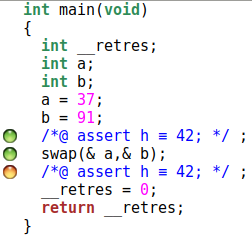
\includegraphics[scale=0.5]{2-2-2-swap-1.png}
\caption{Échec de preuve sur une globale non concernée par l'appel à
\texttt{swap}}
\end{figure}

En effet, nous n'avons pas spécifié les effets de bords autorisés pour
notre fonction. Pour spécifier les effets de bords, nous utilisons la
clause \texttt{assigns} qui fait partie des post-conditions de la
fonction. Elle nous permet de spécifier quels éléments \textbf{non
locaux} (on vérifie bien des effets de bord), sont susceptibles d'être
modifiés par la fonction.

Par défaut, WP considère qu'une fonction a le droit de modifier
n'importe quel élément en mémoire. Nous devons donc préciser ce qu'une
fonction est en droit de modifier. Par exemple pour la fonction swap :

\begin{footnotesize}\begin{Shaded}
\begin{Highlighting}[]
\CommentTok{/*@}
\CommentTok{  requires \textbackslash{}valid(a) && \textbackslash{}valid(b);}
\CommentTok{ }
\CommentTok{  assigns *a, *b;}

\CommentTok{  ensures  *a == \textbackslash{}old(*b) && *b == \textbackslash{}old(*a);}
\CommentTok{*/}
\DataTypeTok{void} \NormalTok{swap(}\DataTypeTok{int}\NormalTok{* a, }\DataTypeTok{int}\NormalTok{* b)\{}
  \DataTypeTok{int} \NormalTok{tmp = *a;}
  \NormalTok{*a = *b;}
  \NormalTok{*b = tmp;}
\NormalTok{\}}
\end{Highlighting}
\end{Shaded}\end{footnotesize}

Si nous rejouons la preuve avec cette spécification, la fonction et les
assertions que nous avions demandées dans le main seront validées par
WP.

Finalement, il peut arriver que nous voulions spécifier qu'une fonction
ne provoque pas d'effets de bords. Ce cas est précisé en donnant
\texttt{\textbackslash{}nothing} à \texttt{assigns} :

\begin{footnotesize}\begin{Shaded}
\begin{Highlighting}[]
\CommentTok{/*@}
\CommentTok{  requires \textbackslash{}valid_read(a) && \textbackslash{}valid_read(b);}

\CommentTok{  assigns  \textbackslash{}nothing;}

\CommentTok{  ensures \textbackslash{}result == *a || \textbackslash{}result == *b;}
\CommentTok{  ensures \textbackslash{}result >= *a && \textbackslash{}result >= *b;}
\CommentTok{*/}
\DataTypeTok{int} \NormalTok{max_ptr(}\DataTypeTok{int}\NormalTok{* a, }\DataTypeTok{int}\NormalTok{* b)\{}
  \KeywordTok{return} \NormalTok{(*a > *b) ? *a : *b ;}
\NormalTok{\}}
\end{Highlighting}
\end{Shaded}\end{footnotesize}

Le lecteur pourra maintenant reprendre les exemples précédents y
intégrer la bonne clause \texttt{assigns} ;) .

\subsubsection{Séparation des zones de la
mémoire}\label{suxe9paration-des-zones-de-la-muxe9moire}

Les pointeurs apportent le risque d'aliasing (plusieurs pointeurs ayant
accès à la même zone de mémoire). Si dans certaines fonctions, cela ne
pose pas de problème, par exemple dans le cas où nous passons les deux
mêmes pointeurs à notre fonction \texttt{swap} où la spécification est
toujours vérifiée par le code source. Dans d'autre cas, ce n'est pas si
simple :

\begin{footnotesize}\begin{Shaded}
\begin{Highlighting}[]
\CommentTok{#include <limits.h>}

\CommentTok{/*@}
\CommentTok{  requires \textbackslash{}valid(a) && \textbackslash{}valid_read(b);}
\CommentTok{  assigns  *a;}
\CommentTok{  ensures  *a == \textbackslash{}old(*a)+ *b;}
\CommentTok{  ensures  *b == \textbackslash{}old(*b);}
\CommentTok{*/}
\DataTypeTok{void} \NormalTok{incr_a_by_b(}\DataTypeTok{int}\NormalTok{* a, }\DataTypeTok{int} \DataTypeTok{const}\NormalTok{* b)\{}
  \NormalTok{*a += *b;}
\NormalTok{\}}
\end{Highlighting}
\end{Shaded}\end{footnotesize}

Si nous demandons à WP de prouver cette fonction, nous obtenons le
résultat suivant :

\begin{figure}[htbp]
\centering
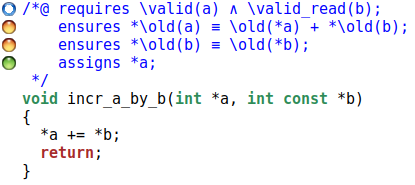
\includegraphics[scale=0.5]{2-2-2-incr_a_by_b-1.png}
\caption{Échec de preuve : risque d'aliasing}
\end{figure}

La raison est simplement que rien ne garantit que le pointeur \texttt{a}
est bien différent du pointeur \texttt{b}. Or, si les pointeurs sont
égaux,

\begin{itemize}
\tightlist
\item
  la propriété \texttt{*a\ ==\ \textbackslash{}old(*a)\ +\ *b} signifie
  en fait \texttt{*a\ ==\ \textbackslash{}old(*a)\ +\ *a}, ce ne peut
  être vrai que si l'ancienne valeur pointée par \texttt{a} était 0, ce
  qu'on ne sait pas,
\item
  la propriété \texttt{*b\ ==\ \textbackslash{}old(*b)} n'est pas
  validée car potentiellement, nous la modifions.
\end{itemize}

\begin{zdsexampleblock}{Pourquoi la clause assign est-elle validée ?}
  C'est simplement dû au fait, qu'il n'y a
  bien que la zone mémoire pointée par \texttt{a} qui est
  modifiée étant donné que si \texttt{a\ !=\ b} nous ne modifions bien
  que cette zone et que si \texttt{a\ ==\ b}, il n'y a toujours
  que cette zone, et pas une autre.
\end{zdsexampleblock}
  
Pour assurer que les pointeurs sont bien sur des zones séparées de
mémoire, ACSL nous offre le prédicat
\texttt{\textbackslash{}separated(p1,\ ...,\ pn)} qui reçoit en entrée
un certain nombre de pointeurs et qui va nous assurer qu'ils sont deux à
deux disjoints. Ici, nous spécifierions :

\begin{footnotesize}\begin{Shaded}
\begin{Highlighting}[]
\CommentTok{#include <limits.h>}

\CommentTok{/*@}
\CommentTok{  requires \textbackslash{}valid(a) && \textbackslash{}valid_read(b);}
\CommentTok{  requires \textbackslash{}separated(a, b);}
\CommentTok{  assigns  *a;}
\CommentTok{  ensures  *a == \textbackslash{}old(*a)+ *b;}
\CommentTok{  ensures  *b == \textbackslash{}old(*b);}
\CommentTok{*/}
\DataTypeTok{void} \NormalTok{incr_a_by_b(}\DataTypeTok{int}\NormalTok{* a, }\DataTypeTok{int} \DataTypeTok{const}\NormalTok{* b)\{}
  \NormalTok{*a += *b;}
\NormalTok{\}}
\end{Highlighting}
\end{Shaded}\end{footnotesize}

Et cette fois, la preuve est effectuée :

\begin{figure}[htbp]
\centering
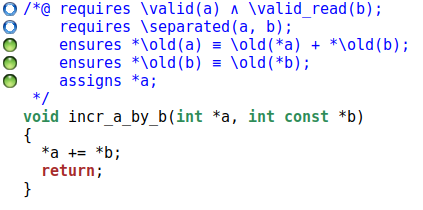
\includegraphics[scale=0.5]{2-2-2-incr_a_by_b-2.png}
\caption{Résolution des problèmes d'aliasing}
\end{figure}

\section{Comportements}\label{comportements}

Il peut arriver qu'une fonction ait divers comportements potentiellement
très différents en fonction de l'entrée. Un cas typique est la réception
d'un pointeur vers une ressource optionnelle : si le pointeur est
\texttt{NULL}, nous aurons un certain comportement et un comportement
complètement différent s'il ne l'est pas.

Nous avons déjà vu une fonction qui avait des comportements différents,
la fonction \texttt{abs}. Nous allons la reprendre comme exemple. Les
deux comportements que nous pouvons isoler sont le cas où la valeur est
positive et le cas où la valeur est négative.

Les comportements nous servent à spécifier les différents cas pour les
post-conditions. Nous les introduisons avec le mot-clé
\texttt{behavior}. Chaque comportement se voit attribuer un nom, les
suppositions du cas que nous traitons introduites par le mot clé
\texttt{assumes} et la post-condition associée. Finalement, nous pouvons
également demander à WP de vérifier le fait que les comportements sont
disjoints (pour garantir le déterminisme) et complets.

Les comportements sont disjoints si pour toute entrée de la fonction,
elle ne correspond aux suppositions (assumes) que d'un seul
comportement. Les comportements sont complets si les suppositions
recouvrent bien tout le domaine des entrées.

Par exemple pour \texttt{abs} :

\begin{footnotesize}\begin{Shaded}
\begin{Highlighting}[]
\CommentTok{/*@}
\CommentTok{  requires val > INT_MIN;}
\CommentTok{  assigns  \textbackslash{}nothing;}

\CommentTok{  behavior pos:}
\CommentTok{    assumes 0 <= val;}
\CommentTok{    ensures \textbackslash{}result == val;}
\CommentTok{  }
\CommentTok{  behavior neg:}
\CommentTok{    assumes val < 0;}
\CommentTok{    ensures \textbackslash{}result == -val;}
\CommentTok{ }
\CommentTok{  complete behaviors;}
\CommentTok{  disjoint behaviors;}
\CommentTok{*/}
\DataTypeTok{int} \NormalTok{abs(}\DataTypeTok{int} \NormalTok{val)\{}
  \KeywordTok{if}\NormalTok{(val < }\DecValTok{0}\NormalTok{) }\KeywordTok{return} \NormalTok{-val;}
  \KeywordTok{return} \NormalTok{val;}
\NormalTok{\}}
\end{Highlighting}
\end{Shaded}\end{footnotesize}

Pour comprendre ce que font précisément \texttt{complete} et
\texttt{disjoint}, il est utile d'expérimenter deux possibilités :

\begin{itemize}
\tightlist
\item
  remplacer la supposition de \og{}pos\fg{} par
  \texttt{val\ \textgreater{}\ 0} auquel cas les comportements seront
  disjoints mais incomplets (il nous manquera le cas
  \texttt{val\ ==\ 0})
\item
  remplacer la supposition de \og{}neg\fg{} par \texttt{val\ \textless{}=\ 0}
  auquel cas les comportements seront complets mais non disjoints (le
  cas \texttt{val\ ==\ 0}) sera présent dans les deux comportements.
\end{itemize}

\begin{zdsalertblock}{Attention}
  Même si \texttt{assigns} est une
  post-condition, à ma connaissance, il n'est pas possible de
  mettre des \texttt{assigns} pour chaque behavior. Si nous avons
  besoin d'un tel cas, nous spécifions :
  \begin{itemize}
  \item \texttt{assigns} avant les behavior (comme dans notre exemple) avec
    tout élément non-local susceptible d'être modifié,
  \item en post-condition de chaque behavior les éléments qui ne sont
    finalement pas modifiés en les indiquant égaux à leur
    ancienne (\texttt{\textbackslash{}old}) valeur.
  \end{itemize}
\end{zdsalertblock}

Les comportements sont très utiles pour simplifier l'écriture de
spécifications quand les fonctions ont des effets très différents en
fonction de leurs entrées. Sans eux, les spécifications passent
systématiquement par des implications traduisant la même idée mais dont
l'écriture et la lecture sont plus difficiles (nous sommes susceptibles
d'introduire des erreurs).

D'autre part, la traduction de la complétude et de la disjonction
devraient être écrites manuellement, ce qui serait fastidieux et une
nouvelle fois source d'erreurs.

\section{Modularité du WP}\label{modularituxe9-du-wp}

Pour terminer cette partie nous allons parler de la composition des
appels de fonctions et commencer à entrer dans les détails de
fonctionnement de WP. Nous allons en profiter pour regarder comment se
traduit le découpage de nos programmes en fichiers lorsque nous voulons
les spécifier et les prouver avec WP.

Notre but sera de prouver la fonction \texttt{max\_abs} qui renvoie les
maximum entre les valeurs absolues de deux valeurs :

\begin{footnotesize}\begin{Shaded}
\begin{Highlighting}[]
\DataTypeTok{int} \NormalTok{max_abs(}\DataTypeTok{int} \NormalTok{a, }\DataTypeTok{int} \NormalTok{b)\{}
  \DataTypeTok{int} \NormalTok{abs_a = abs(a);}
  \DataTypeTok{int} \NormalTok{abs_b = abs(b);}

  \KeywordTok{return} \NormalTok{max(abs_a, abs_b);}
\NormalTok{\}}
\end{Highlighting}
\end{Shaded}\end{footnotesize}

Commençons par (sur-)découper nos précédentes fonctions en couples
headers/source pour \texttt{abs} et \texttt{max}. Cela donne pour
\texttt{abs} :

Fichier abs.h :

\begin{footnotesize}\begin{Shaded}
\begin{Highlighting}[]
\CommentTok{#ifndef _ABS}
\CommentTok{#define _ABS}

\CommentTok{#include <limits.h>}

\CommentTok{/*@}
\CommentTok{  requires val > INT_MIN;}
\CommentTok{  assigns  \textbackslash{}nothing;}

\CommentTok{  behavior pos:}
\CommentTok{    assumes 0 <= val;}
\CommentTok{    ensures \textbackslash{}result == val;}
\CommentTok{  }
\CommentTok{  behavior neg:}
\CommentTok{    assumes val < 0;}
\CommentTok{    ensures \textbackslash{}result == -val;}
\CommentTok{ }
\CommentTok{  complete behaviors;}
\CommentTok{  disjoint behaviors;}
\CommentTok{*/}
\DataTypeTok{int} \NormalTok{abs(}\DataTypeTok{int} \NormalTok{val);}

\CommentTok{#endif}
\end{Highlighting}
\end{Shaded}\end{footnotesize}

Fichier abs.c

\begin{footnotesize}\begin{Shaded}
\begin{Highlighting}[]
\CommentTok{#include "abs.h"}

\DataTypeTok{int} \NormalTok{abs(}\DataTypeTok{int} \NormalTok{val)\{}
  \KeywordTok{if}\NormalTok{(val < }\DecValTok{0}\NormalTok{) }\KeywordTok{return} \NormalTok{-val;}
  \KeywordTok{return} \NormalTok{val;}
\NormalTok{\}}
\end{Highlighting}
\end{Shaded}\end{footnotesize}

Nous découpons en mettant le contrat de la fonction dans le header. Le
but de ceci est de pouvoir, lorsque nous aurons besoin de la fonction
dans un autre fichier, importer la spécification en même temps que la
déclaration de celle-ci. En effet, WP en aura besoin pour montrer que
les appels à cette fonction sont valides.

Nous pouvons créer un fichier sous le même formatage pour la fonction
\texttt{max}. Dans les deux cas, nous pouvons ré-ouvrir le fichier
source (pas besoin de spécifier les fichiers headers dans la ligne de
commande) avec Frama-C et remarquer que la spécification est bien
associée à la fonction et que nous pouvons la prouver.

Maintenant, nous pouvons préparer le terrain pour la fonction
\texttt{max\_abs}. Dans notre header :

\begin{footnotesize}\begin{Shaded}
\begin{Highlighting}[]
\CommentTok{#ifndef _MAX_ABS}
\CommentTok{#define _MAX_ABS}

\DataTypeTok{int} \NormalTok{max_abs(}\DataTypeTok{int} \NormalTok{a, }\DataTypeTok{int} \NormalTok{b);}

\CommentTok{#endif}
\end{Highlighting}
\end{Shaded}\end{footnotesize}

Et dans le source :

\begin{footnotesize}\begin{Shaded}
\begin{Highlighting}[]
\CommentTok{#include "max_abs.h"}
\CommentTok{#include "max.h"}
\CommentTok{#include "abs.h"}

\DataTypeTok{int} \NormalTok{max_abs(}\DataTypeTok{int} \NormalTok{a, }\DataTypeTok{int} \NormalTok{b)\{}
  \DataTypeTok{int} \NormalTok{abs_a = abs(a);}
  \DataTypeTok{int} \NormalTok{abs_b = abs(b);}

  \KeywordTok{return} \NormalTok{max(abs_a, abs_b);}
\NormalTok{\}}
\end{Highlighting}
\end{Shaded}\end{footnotesize}

Et ouvrir ce dernier fichier dans Frama-C. Si nous regardons le panneau
latéral, nous pouvons voir que les fichiers header que nous avons inclus
dans le fichier \texttt{abs\_max.c} y apparaissent et que les contrats
de fonction sont décorés avec des pastilles particulières (vertes et
bleues) :

\begin{figure}[htbp]
\centering
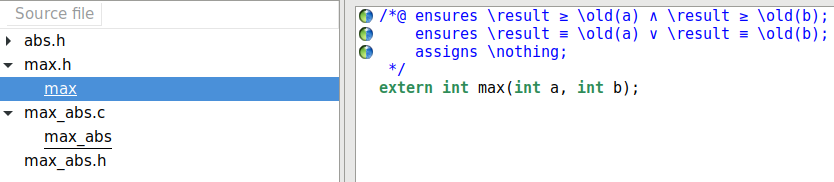
\includegraphics[scale=0.5]{2-4-max_abs.png}
\caption{Le contrat de \texttt{max} est valide par hypothèse}
\end{figure}

Ces pastilles nous disent qu'en l'absence d'implémentation, les
propriétés sont supposées vraies. Et c'est une des forces de la preuve
déductive de programmes par rapport à certaines autres méthodes
formelles, les fonctions sont vérifiées en isolation les unes des
autres.

En dehors de la fonction, sa spécification est considérée comme étant
vérifiée : nous ne cherchons pas à reprouver que la fonction fait bien
son travail à chaque appel, nous nous contenterons de vérifier que les
pré-conditions sont réunies au moment de l'appel. Cela donne donc des
preuves très modulaires et donc des spécifications plus facilement
réutilisables. Évidemment, si notre preuve repose sur la spécification
d'une autre fonction, cette fonction doit-elle même être vérifiable pour
que la preuve soit formellement complète. Mais nous pouvons également
vouloir simplement vers confiance à une bibliothèque externe sans la
prouver.

Finalement, le lecteur pourra essayer de spécifier la fonction
\texttt{max\_abs}.

La spécification peut ressembler à ceci (j'ai mis l'implémentation avec
pour rappel) :

\begin{footnotesize}\begin{Shaded}
\begin{Highlighting}[]
\CommentTok{/*@}
\CommentTok{  requires a > INT_MIN;}
\CommentTok{  requires b > INT_MIN;}

\CommentTok{  assigns \textbackslash{}nothing;}

\CommentTok{  ensures \textbackslash{}result >= 0;}
\CommentTok{  ensures \textbackslash{}result >= a && \textbackslash{}result >= -a && \textbackslash{}result >= b && \textbackslash{}result >= -b;}
\CommentTok{  ensures \textbackslash{}result == a || \textbackslash{}result == -a || \textbackslash{}result == b || \textbackslash{}result == -b;}
\CommentTok{*/}
\DataTypeTok{int} \NormalTok{abs_max(}\DataTypeTok{int} \NormalTok{a, }\DataTypeTok{int} \NormalTok{b)\{}
  \DataTypeTok{int} \NormalTok{abs_a = abs(a);}
  \DataTypeTok{int} \NormalTok{abs_b = abs(b);}

  \KeywordTok{return} \NormalTok{max(abs_a, abs_b);}
\NormalTok{\}}
\end{Highlighting}
\end{Shaded}\end{footnotesize}

Pendant cette partie, nous avons vu comment spécifier les fonctions par
l'intermédiaire de leurs contrats, à savoir leurs pré et
post-conditions, ainsi que quelques fonctionnalités offertes par ACSL
pour exprimer ces propriétés. Nous avons également vu pourquoi il est
important d'être précis dans la spécification et comment l'introduction
des comportements nous permet de ne pas surcharger l'écriture pour
autant.

En revanche, nous n'avons pas encore vu un point important : la
spécification des boucles. Avant d'entamer cette partie, nous devrions
regarder plus précisément comment fonctionne l'outil WP.

\chapter{Instructions basiques et structures de
contrôle}\label{instructions-basiques-et-structures-de-contruxf4le}

\begin{zdsblock}{Information}
  Cette partie est plus formelle que ce
  nous avons vu jusqu'à maintenant. Si le lecteur souhaite se
  concentrer sur l'utilisation de l'outil, l'introduction de ce
  chapitre et les deux premières sections (sur les instructions de base et
  \og{}le bonus stage\fg{}) sont dispensables. Si ce que nous avons
  présenté jusqu'à maintenant vous a semblé ardu sur un plan
  formel, il est également possible de réserver l'introduction
  et ces deux sections pour une deuxième lecture.
  
  Les sections sur les boucles sont en revanches indispensables. Les
  éléments plus formels de ces sections seront signalés.
\end{zdsblock}
  
Pour chaque notion en programmation C, Nous associerons la règle
d'inférence qui lui correspond, la règle utilisée de calcul de plus
faible pré-conditions qui la régit, et des exemples d'utilisation. Pas
forcément dans cet ordre et avec plus ou moins de liaison avec l'outil.
Les premiers points seront plus focalisés sur la théorie que sur
l'utilisation car ce sont les plus simples, au fur et à mesure, nous
nous concentrerons de plus en plus sur l'outil, en particulier quand
nous attaquerons le point concernant les boucles.

\subsection{Règle d'inférence}\label{ruxe8gle-dinfuxe9rence}

Une règle d'inférence est de la forme :

\begin{center} \(\dfrac{P_1 \quad ... \quad P_n}{C}\) \end{center}

Et signifie que pour assurer que la conclusion \(C\) est vraie, il faut
d'abord savoir que les prémisses \(P_1\), \ldots{}, et \(P_n\) sont
vraies. Quand il n'y a pas de prémisses :

\begin{center} \(\dfrac{}{\quad C \quad}\) \end{center}

Alors, il n'y a rien à assurer pour conclure que \(C\) est vraie.

Inversement, pour prouver qu'une certaine prémisse est vraie, il peut
etre nécessaire d'utiliser une autre règle d'inférence, ce qui nous
donnerait quelque chose comme :

\begin{center}
\(\dfrac{\dfrac{}{\quad P_1\quad} \quad \dfrac{P_{n_1}\quad P_{n_2}}{P_n}}{C}\)
\end{center}

Ce qui nous construit progressivement l'arbre de déduction de notre
raisonnement. Dans notre raisonnement, les prémisses et conclusions
manipulées seront généralement des triplets de Hoare.

\subsection{Triplet de Hoare}\label{triplet-de-hoare}

Revenons sur la notion de triplet de Hoare :

\begin{center} \(\{ P \} C \{ Q \}\) \end{center}

Nous l'avons vu en début de tutoriel, ce que nous propose Dijkstra,
c'est un moyen de calculer à partir d'une post-condition \(Q\) et d'une
commande ou d'une liste de commandes \(C\), la pré-condition minimale
assurant \(Q\) après \(C\). Plus formellement, l'idée est la suivante :

\begin{center} \(\{\ wp(C,Q)\ \} C \{ Q \}\) \end{center}

Nous pouvons considérer que \(wp\) est une fonction qui, à une
post-condition voulue et un programme ou une instruction, nous associe
la plus faible pré-condition qui permet de l'assurer. Nous utiliserons
donc cette notation pour définir le calcul correspondant à une/des
instructions :

\(wp(Instruction(s), Post) = WeakestPrecondition\)

Nous utiliserons souvent des assertions ACSL pour présenter les notions
à venir :

\begin{footnotesize}\begin{Shaded}
\begin{Highlighting}[]
\CommentTok{//@ assert ma_propriete ;}
\end{Highlighting}
\end{Shaded}\end{footnotesize}

\section{Affectation, séquence et
conditionnelle}\label{affectation-suxe9quence-et-conditionnelle}

\subsection{Affectation}\label{affectation}

L'affectation est l'opération la plus basique que l'on puisse avoir dans
un langage (mise à part l'opération \og{}ne rien faire\fg{} qui manque
singulièrement d'intérêt). Le calcul de plus faible pré-condition
associé est le suivant :

\begin{center} \(wp(x = E , Post) = Post[x \leftarrow E]\) \end{center}

Où la notation \(P[x \leftarrow E]\) signifie \og{}la propriété \(P\) où
\(x\) est remplacé par \(E\)\fg{}. Ce qui correspond ici à \og{}la
post-condition \(Post\) où \(x\) a été remplacé par \(E\)\fg{}. Dans
l'idée, pour que la formule en post-condition d'une affectation de \(x\)
à \(E\) soit vraie, il faut qu'elle soit vraie en remplaçant chaque
occurrence de \(x\) dans la formule par \(E\). Par exemple :

\begin{center} \(\{P\}\quad x = 43*c \quad \{ x = 258 \}\) \end{center}

\begin{center} \(P = wp(x = 43*c , \{x = 258\}) = \{43*c = 258\}\)
\end{center}

Ce qui finalement nous donnerait cette écriture :

\begin{center} \(\{43*c = 258\}\quad x = 43*c\quad \{ x = 258 \}\)
\end{center}

Pour calculer la pré-condition de l'affectation, nous avons remplacé
chaque occurrence de \(x\) dans la post-condition, par la valeur
\(E = 43*c\) affectée. Nous pourrions alors déduire qu'avant exécution c
doit valoir 6.

La règle d'inférence prenant en compte le calcul de plus faible
pré-condition est donc la suivante :

\begin{center}
\(\dfrac{}{\{Q[x \leftarrow E] \}\quad x = E \quad\{ Q \}}\)
\end{center}

Nous noterons qu'il n'y a pas de prémisse à vérifier. Cela veut-il dire
que le triplet est nécessairement vrai ? Oui. Mais cela ne dit pas si la
pré-condition est respectée par le programme où se trouve l'instruction,
ni que cette pré-condition est possible. C'est ce travail qu'effectuent
ensuite les prouveurs automatiques.

Par exemple, nous pouvons demander la vérification de la ligne suivante
avec Frama-C :

\begin{footnotesize}\begin{Shaded}
\begin{Highlighting}[]
\DataTypeTok{int} \NormalTok{a = }\DecValTok{42}\NormalTok{;}
\CommentTok{//@ assert a == 42;}
\end{Highlighting}
\end{Shaded}\end{footnotesize}

Ce qui est, bien entendu, prouvé directement par Qed car c'est une
simple application de la règle de l'affectation.

\begin{zdsblock}{Information}
  Notons que d'après la norme C,
  l'opération d'affectation est une expression et non une
  instruction. C'est ce qui nous permet par exemple d'écrire
  \texttt{if(\ (a\ =\ foo())\ ==\ 42)}. Dans Frama-C, une affectation sera
  toujous une instruction. En effet, si une affectation est
  présente au sein d'une expression plus complexe, le module de
  création de l'arbre de syntaxe abstraite du programme analysé
  effectue une étape de normalisation qui crée systématiquement
  une instruction séparée.
\end{zdsblock}

\subsection{Séquence d'instructions}\label{suxe9quence-dinstructions}

Pour qu'une instruction soit valide, il faut que sa pré-condition nous
permette, par cette instruction, de passer à la post-condition voulue.
Maintenant, nous avons besoin d'enchaîner ce processus d'une instruction
à une autre. L'idée est alors que la post-condition assurée par la
première instruction soit compatible avec la pré-condition demandée par
la deuxième et que ce processus puisse se répéter pour la troisième
instruction, etc.

Nous associons la règle d'inférence suivante à cette idée :

\begin{center}
\(\dfrac{\{P\}\quad S1 \quad \{R\} \ \ \ \{R\}\quad S2 \quad \{Q\}}{\{P\}\quad S1 ;\ S2 \quad \{Q\}}\)
\end{center}

Pour vérifier que la séquence d'instruction \(S1;\ S2\) (NB : Où \(S1\)
et \(S2\) peuvent elles-mêmes être des séquences d'instruction), nous
passons par une propriété intermédiaire qui est à la fois la
pré-condition de \(S2\) et la post-condition de \(S1\). Le calcul de
plus faible pré-condition nous dit simplement que cette propriété
intermédiaire est trouvée par calcul de pré-condition de la deuxième
instruction. La plus faible pré-condition de l'ensemble étant donc
déterminée comme ceci :

\begin{center} \(wp(S1;\ S2 , Post) = wp(S1, wp(S2, Post) )\)
\end{center}

Le plugin WP de Frama-C fait ce calcul pour nous, c'est pour cela que
nous n'avons pas besoin d'écrire les assertions entre chaque ligne de
code.

\begin{footnotesize}\begin{Shaded}
\begin{Highlighting}[]
\DataTypeTok{int} \NormalTok{main()\{}
  \DataTypeTok{int} \NormalTok{a = }\DecValTok{42}\NormalTok{;}
  \DataTypeTok{int} \NormalTok{b = }\DecValTok{37}\NormalTok{;}

  \DataTypeTok{int} \NormalTok{c = a+b; }\CommentTok{// i:1}
  \NormalTok{a -= c;      }\CommentTok{// i:2}
  \NormalTok{b += a;      }\CommentTok{// i:3}

  \CommentTok{//@assert b == 0 && c == 79;}
\NormalTok{\}}
\end{Highlighting}
\end{Shaded}\end{footnotesize}

\subsubsection{Arbre de preuve}\label{arbre-de-preuve}

Notons que lorsque nous avons plus de deux instructions, nous pouvons
simplement considérer que la dernière instruction est la seconde
instruction de notre règle et que toutes les instructions qui la précède
forme la première \og{}instruction\fg{}. De cette manière nous remontons bien
les instructions une à une dans notre raisonnement, par exemple avec le
programme précédent :

\begin{center}
\begin{tabular}{ccc}
  $\{P\}\quad i_1 ; \quad \{Q_{-2}\}$ & $\{Q_{-2}\}\quad i_2 ; \quad \{Q_{-1}\}$ & \\
  \cline{1-2}
  \multicolumn{2}{c}{$\{P\}\quad i\_1 ; \quad i\_2 ; \quad \{Q_{-1}\}$} & $\{Q_{-1}\} \quad i_3 ; \quad \{Q\}$\\
  \hline
  \multicolumn{3}{c}{$\{P\}\quad i\_1 ; \quad i\_2 ; \quad i\_3; \quad \{ Q \}$}
\end{tabular}
\end{center}

Nous pouvons par calcul de plus faibles pré-conditions construire la
propriété \(Q_{-1}\) à partir de \(Q\) et \(i_3\), ce qui nous permet de
déduire \(Q_{-2}\), à partir de \(Q_{-1}\) et \(i_2\) et finalement
\(P\) avec \(Q_{-2}\) et \(i_1\).

Nous pouvons maintenant vérifier des programmes comprenant plusieurs
instructions, il est temps d'y ajouter un peu de structure.

\subsection{Règle de la
conditionnelle}\label{ruxe8gle-de-la-conditionnelle}

Pour qu'un branchement conditionnel soit valide, il faut que la
post-condition soit atteignable par les deux banches, depuis la même
pré-condition, à ceci près que chacune des branches aura une information
supplémentaire : le fait que la condition était vraie dans un cas et
fausse dans l'autre.

Comme avec la séquence d'instruction, nous aurons donc deux points à
vérifier (pour éviter de confondre les accolades, j'utilise la syntaxe
\(if\ B\ then\ S1\ else\ S2\)) :

\begin{center}
\(\dfrac{\{P \wedge B\}\quad S1\quad \{Q\} \quad \quad \{P \wedge \neg B\}\quad S2\quad \{Q\}}{\{P\}\quad if\quad B\quad then\quad S1\quad else\quad S2 \quad \{Q\}}\)
\end{center}

Nos deux prémisses sont donc la vérification que lorque nous avons la
pré-condition et que nous passons dans la branche \texttt{if}, nous
atteignons bien la post-condition, et que lorsque nous avons la
pré-condition et que nous passons dans la branche \texttt{else}, nous
obtenons bien également la post-condition.

Le calcul de pré-condition correspondant est le suivant :

\begin{center}
\(wp(if\ B\ then\ S1\ else\ S2 , Post) = (B \Rightarrow wp(S1, Post)) \wedge (\neg B \Rightarrow wp(S2, Post))\)
\end{center}

À savoir que \(B\) doit impliquer la pré-condition la plus faible de
\(S1\), pour pouvoir l'exécuter sans erreur vers la post-condition, et
que \(\neg B\) doit impliquer la pré-condition la plus faible de \(S2\)
(pour la même raison).

\subsubsection{\texorpdfstring{Bloc \texttt{else}
vide}{Bloc else vide}}\label{bloc-else-vide}

En suivant cette définition, si le \texttt{else} ne fait rien, alors la
règle d'inférence est de la forme suivante, en remplaçant \(S2\) par une
instruction \og{}ne rien faire\fg{}.

\begin{center}
\(\dfrac{\{P \wedge B\}\quad S1\quad \{Q\} \quad \quad \{P \wedge \neg B\}\quad skip\quad \{Q\}}{\{P\}\quad if\quad B\quad then\quad S1\quad else\quad skip \quad \{Q\}}\)
\end{center}

Le triplet pour le \texttt{else} est :

\begin{center} \(\{P \wedge \neg B\}\quad skip\quad \{Q\}\)
\end{center}

Ce qui veut dire que nous devons avoir :

\begin{center} \(Pre \wedge \neg B \Rightarrow Q\) \end{center}

En résumé, si la condition du \texttt{if} est fausse, cela veut dire que
la post-condition de l'instruction conditionnelle globale est déjà
vérifiée avant de rentrer dans le \texttt{else} (puisqu'il ne fait
rien).

Par exemple, nous pourrions vouloir remettre une configuration \(c\) à
une valeur par défaut si elle a mal été configurée par un utilisateur du
programme :

\begin{footnotesize}\begin{Shaded}
\begin{Highlighting}[]
\DataTypeTok{int} \NormalTok{c;}

\CommentTok{// ... du code ...}

\KeywordTok{if}\NormalTok{(c < }\DecValTok{0} \NormalTok{|| c > }\DecValTok{15}\NormalTok{)\{}
  \NormalTok{x = }\DecValTok{0}\NormalTok{;}
\NormalTok{\}}
\CommentTok{//@ assert 0 <= c <= 15;}
\end{Highlighting}
\end{Shaded}\end{footnotesize}

Soit :

\(wp(if \neg (c \in [0;15])\ then\ c := 0, \{c \in [0;15]\})\)

\(= (\neg (c \in [0;15])\Rightarrow wp(c := 0, \{c \in [0;15]\})) \wedge (c \in [0;15]\Rightarrow wp(skip, \{c \in [0;15]\}))\)

\(= (\neg (c \in [0;15]) \Rightarrow 0 \in [0;15]) \wedge (c \in [0;15] \Rightarrow c \in [0;15])\)

\(= (\neg (c \in [0;15]) \Rightarrow true) \wedge true\)

La formule est bien vérifiable : quelle que soit l'évaluation de
\(\neg (c \in [0;15])\) l'implication sera vraie.

\subsubsection{Relation avec l'arbre de preuve et
modularité.}\label{relation-avec-larbre-de-preuve-et-modularituxe9.}

Si l'on remplace dans notre règle d'inférence, les occurrences de \(P\)
par le calcule de plus faible pré-condition correspondant \(Q\), nous
obtenons (en notant l'instruction conditionnelle complète \(c\)) :

\begin{center}
\(\dfrac{\{wp(c,Q) \wedge B\}\quad S1\quad \{Q\} \quad \quad \{wp(c,Q) \wedge \neg B\}\quad S2\quad \{Q\}}{\{wp(c,Q)\}\quad c\quad \{Q\}}\)\end{center}

Or si l'on prend l'arbre de preuve qui correspond par exemple à \(S1\)
(c'est similaire pour \(S2\)) et que nous y faisons le remplacement de
\(wp(c,Q)\), nous obtenons :

\begin{center}
\(\{ (B \Rightarrow wp(S1,Q)) \wedge (\neg B \Rightarrow wp(S2,Q)) \wedge B \} \quad S1 \quad \{Q\}\)
\end{center}

Ce qui n'est pas très modulaire : nous devons parler du calcul de plus
faible pré-condition de \(S2\) dans la preuve qui correspond à \(S1\).
En fait, en simplifiant la formule nous obtenons :

\begin{center} \(\{ wp(S1,Q) \wedge B \} \quad S1 \quad \{Q\}\)
\end{center}

Or, \(wp(S1,Q) \wedge B \Rightarrow wp(S1,Q)\). Et nous allons voir dans
la section suivante une règle d'inférence, la règle de conséquence, qui
nous permet de construire l'arbre de déduction suivant :

\begin{center}
\(\dfrac{wp(S1,Q) \wedge B \Rightarrow wp(S1,Q)\quad\quad\{ wp(S1,Q) \} \quad S1 \quad \{Q\}}{\{ wp(S1,Q) \wedge B \} \quad S1 \quad \{Q\}}\)
\end{center}

Nous laissant à prouver :

\begin{center} \(\{ wp(S1,Q) \} \quad S1 \quad \{Q\}\) \end{center}

qui est bien le calcul de plus pré-condition de \(S1\), ne nécessitant
alors plus de raisonner à propos de la pré-condition de \(S2\) qui nous
ennuyait.

\section{{[}Bonus Stage{]} Conséquence et
constance}\label{bonus-stage-consuxe9quence-et-constance}

\subsection{Règle de conséquence}\label{ruxe8gle-de-consuxe9quence}

Parfois, il peut être utile pour la preuve d'affaiblir une
post-condition ou de renforcer une pré-condition. Si la première sera
souvent établie par nos soins pour faciliter le travail du prouveur, la
seconde est plus souvent vérifiée par l'outil à l'issu du calcul de plus
faible pré-condition.

La règle d'inférence en logique de Hoare est la suivante :

\begin{center}\(\dfrac{P \Rightarrow SP \quad \{SP\}\quad c\quad \{WQ\} \quad WQ \Rightarrow Q}{\{P\}\quad c \quad \{Q\}}\)\end{center}

(Nous noterons que les prémisses, ici, ne sont pas seulement des
triplets de Hoare mais également des formules à vérifier)

Par exemple, si notre post-condition est trop complexe, elle risque de
générer une plus faible pré-condition trop compliquée et de rendre le
calcul des prouveurs difficile. Nous pouvons alors créer une
post-condition intermédiaire \(WQ\), plus simple, mais plus restreinte
et impliquant la vraie post-condition. C'est la partie
\(WQ \Rightarrow Q\).

Inversement, le calcul de pré-condition générera généralement une
formule compliquée et souvent plus faible que la pré-condition que nous
souhaitons accepter en entrée. Dans ce cas, c'est notre outil qui
s'occupera de vérifier l'implication entre ce que nous voulons et ce qui
est nécessaire pour que notre code soit valide. C'est la partie
\(P \Rightarrow SP\).

\subsection{Règle de constance}\label{ruxe8gle-de-constance}

Certaines séquences d'instructions peuvent concerner et faire intervenir
des variables différentes. Ainsi, il peut arriver que nous initialisions
et manipulions un certain nombre de variables, que nous commencions à
utiliser certaines d'entre elles, puis que nous les délaissions au
profit d'autres pendant un temps. Quand un tel cas apparaît, nous avons
envie que l'outil ne se préoccupe que des variables qui sont
susceptibles d'être modifiées pour avoir des propriétés les plus légères
possibles.

La règle d'inférence qui définit ce raisonnement est la suivante :

\begin{center}
\(\dfrac{\{P\}\quad c\quad \{Q\}}{\{P \wedge R\}\quad c\quad \{Q \wedge R\}}\)
\end{center}

Où \(c\) ne modifie aucune variable entrant en jeu dans \(R\). Ce qui
nous dit : \og{}pour vérifier le triplet, débarrassons nous des parties de
la formule qui concerne des variables qui ne sont pas manipulées par
\(c\) et prouvons le nouveau triplet\fg{}.

\section{Les boucles}\label{les-boucles}

Les boucles ont besoin d'un traitement de faveur dans la vérification
déductive de programmes. Ce sont les seules structures de contrôle qui
vont nécessiter un travail conséquent de notre part. Nous ne pouvons pas
y échapper car sans les boucles nous pouvons difficilement prouver des
programmes intéressants.

Avant de s'intéresser à la spécification des boucles, il est légitime de
se poser la question suivante : pourquoi les boucles sont-elles
compliquées ?

\subsection{Induction et invariance}\label{induction-et-invariance}

La nature des boucles rend leur analyse difficile. Lorsque nous faisons
nos raisonnements arrières, il nous faut une règle capable de dire à
partir de la post-condition quelle est la pré-condition d'une certaine
séquence d'instructions. Problème : nous ne pouvons \emph{a priori} pas
déduire combien de fois la boucle va s'exécuter et donc par conséquent,
nous ne pouvons pas non plus savoir combien de fois les variables ont
été modifiées.

Nous allons donc procéder en raisonnant par induction. Nous devons
trouver une propriété qui est vraie avant de commencer la boucle et qui
si elle est vraie en début d'un tour de boucle, sera vraie à la fin (et
donc par extension, au début du tour suivant).

Ce type de propriété est appelé un invariant de boucle. Un invariant de
boucle est une propriété qui doit est vraie avant et après chaque tour
d'une boucle. Par exemple, pour la boucle :

\begin{footnotesize}\begin{Shaded}
\begin{Highlighting}[]
\KeywordTok{for}\NormalTok{(}\DataTypeTok{int} \NormalTok{i = }\DecValTok{0} \NormalTok{; i < }\DecValTok{10} \NormalTok{; ++i)\{ }\CommentTok{/* */} \NormalTok{\}}
\end{Highlighting}
\end{Shaded}\end{footnotesize}

La propriété \(0 <= i <= 10\) est un invariant de la boucle. La
propriété \(-42 <= i <= 42\) est également un invariant de la boucle
(qui est nettement plus imprécis néanmoins). La propriété
\(0 < i <= 10\) n'est pas un invariant, elle n'est pas vraie à l'entrée
de la boucle. La propriété \(0 <= i < 10\) \textbf{n'est pas un
invariant de la boucle}, elle n'est pas vraie à la fin du dernier tour
de la boucle qui met la valeur \(i\) à \(10\).

Le raisonnement produit par l'outil pour vérifier un invariant \(I\)
sera donc :

\begin{itemize}
\tightlist
\item
  vérifions que \(I\) est vrai au début de la boucle (établissement),
\item
  vérifions que \(I\) est vrai avant de commencer un tour, alors \(I\)
  vrai après (préservation).
\end{itemize}

\subsubsection{{[}Formel{]} Règle
d'inférence}\label{formel-ruxe8gle-dinfuxe9rence}

En notant l'invariant \(I\), la règle d'inférence correspondant à la
boucle est définie comme suit :

\begin{center}
\(\dfrac{\{I \wedge B \}\ c\ \{I\}}{\{I\}\ while(B)\{c\}\ \{I \wedge \neg B\}}\)
\end{center}

Et le calcul de plus faible pré-condition est le suivant :

\begin{center}
\(wp(while (B) \{ S \}, Post) = I \wedge ((B \wedge I) \Rightarrow wp(S, I)) \wedge ((\neg B \wedge I) \Rightarrow Post)\)
\end{center}

Détaillons cette formule :

\begin{itemize}
\item
  \begin{enumerate}
  \def\labelenumi{(\arabic{enumi})}
  \tightlist
  \item
    le premier \(I\) correspond à l'établissement de l'invariant, c'est
    vulgairement la \og{}pré-condition\fg{} de la boucle,
  \end{enumerate}
\item
  la deuxième partie de la conjonction
  (\((B \wedge I) \Rightarrow wp(S, I)\)) correspond à la vérification
  du travail effectué par le corps de la boucle :

  \begin{itemize}
  \item
    la pré-condition que nous connaissons du corps de la boucle (notons
    \(KWP\), \og{}Known WP\fg{}) , c'est (\(KWP = B \wedge I\)). Soit le fait
    que nous sommes rentrés dedans (\(B\) est vrai), et que l'invariant
    est respecté à ce moment (\(I\), qui est vrai avant de commencer la
    boucle par 1, et dont veut vérifier qu'il sera vraie en fin de bloc
    de la boucle (2)),
  \item
    \begin{enumerate}
    \def\labelenumi{(\arabic{enumi})}
    \setcounter{enumi}{1}
    \tightlist
    \item
      ce qu'il nous reste à vérifier c'est que \(KWP\) implique la
      pré-condition réelle* du bloc de code de la boucle
      (\(KWP \Rightarrow wp(S, Post)\)). Ce que nous voulons en fin de
      bloc, c'est avoir maintenu l'invariant \(I\) (\(B\) n'est
      peut-être plus vrai en revanche). Donc
      \(KWP \Rightarrow wp(S, I)\), soit
      \((B \wedge I) \Rightarrow wp(S, I)\),
    \end{enumerate}
  \item
    * cela correspond à une application de la règle de conséquence
    expliquée précédemment.
  \end{itemize}
\item
  finalement la dernière partie (\((\neg B \wedge I) \Rightarrow Post\))
  nous dit que le fait d'être sorti de la boucle (\(\neg B\)), tout en
  ayant maintenu l'invariant \(I\), doit impliquer la post-condition
  voulue pour la boucle.
\end{itemize}

\subsubsection{Retour à l'outil}\label{retour-uxe0-loutil}

Il existe des outils capables d'inférer des invariants (pour peu qu'ils
soient simples, les outils automatiques restent limités). Ce n'est pas
le cas de WP. Il nous faut donc écrire nos invariants à la main. Pour
cela nous ajoutons les annotations suivantes en début de boucle :

\begin{footnotesize}\begin{Shaded}
\begin{Highlighting}[]
\DataTypeTok{int} \NormalTok{main()\{}
  \DataTypeTok{int} \NormalTok{i = }\DecValTok{0}\NormalTok{;}
  
  \CommentTok{/*@}
\CommentTok{    loop invariant 0 <= i <= 30;}
\CommentTok{  */}
  \KeywordTok{while}\NormalTok{(i < }\DecValTok{30}\NormalTok{)\{}
    \NormalTok{++i;}
  \NormalTok{\}}
  \CommentTok{//@assert i == 30;}
\NormalTok{\}}
\end{Highlighting}
\end{Shaded}\end{footnotesize}

\begin{zdsalertblock}{Attention}
  \textbf{RAPPEL} : L'invariant est bien : i \textbf{\textless{}=} 30 !
\end{zdsalertblock}

Pourquoi ? Parce que tout au long de la boucle \texttt{i} sera bien
compris entre 0 et 30 \textbf{inclus}. 30 est même la valeur qui nous
permettra de sortir de la boucle. Plus encore, une des propriétés
demandées par le calcul de plus faible pré-conditions sur les boucles
est que lorsque l'on invalide la condition de la boucle, par la
connaissance de l'invariant, on peut prouver la post-condition
(Formellement : \((\neg B \wedge I) \Rightarrow Post\)).

La post-condition de notre boucle est \texttt{i\ ==\ 30}. Et doit être
impliquée par \(\neg\) \texttt{i\ \textless{}\ 30} \(\wedge\)
\texttt{0\ \textless{}=\ i\ \textless{}=\ 30}. Ici, cela fonctionne bien
:
\texttt{i\ \textgreater{}=\ 30\ \&\&\ 0\ \textless{}=\ i\ \textless{}=\ 30\ ==\textgreater{}\ i\ ==\ 30}.
Si l'invariant excluait l'égalité à 30, la post-condition ne serait pas
atteignable.

Une nouvelle fois, nous pouvons jeter un œil à la liste des buts dans WP
Goals :

\begin{figure}[htbp]
\centering
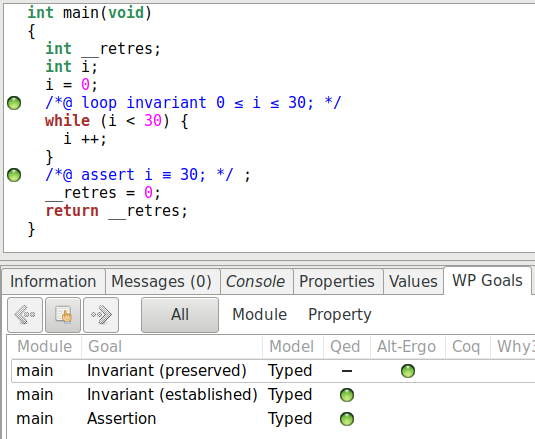
\includegraphics[scale=0.5]{3-3-1-i_30-1.png}
\caption{Obligations générées pour prouver notre boucle}
\end{figure}

Nous remarquons bien que WP décompose la preuve de l'invariant en deux
parties : l'établissement de l'invariant et sa préservation. WP produit
exactement le raisonnement décrit plus haut pour la preuve de
l'assertion. Dans les versions récentes de Frama-C, Qed est devenu
particulièrement puissant, et l'obligation de preuve générée ne le
montre pas (affichant simplement \og{}True\fg{}). En utilisant l'option
\texttt{-wp-no-simpl} au lancement, nous pouvons quand même voir
l'obligation correspondante :

\begin{figure}[htbp]
\centering
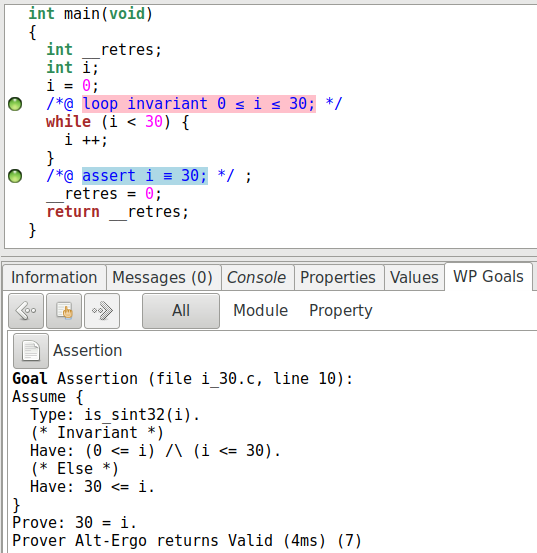
\includegraphics[scale=0.5]{3-3-sortie-boucle.png}
\caption{Preuve de l'assertion par connaissance de l'invariant et
l'invalidation de la condition de boucle}
\end{figure}

Mais notre spécification est-elle suffisante ?

\begin{footnotesize}\begin{Shaded}
\begin{Highlighting}[]
\DataTypeTok{int} \NormalTok{main()\{}
  \DataTypeTok{int} \NormalTok{i = }\DecValTok{0}\NormalTok{;}
  \DataTypeTok{int} \NormalTok{h = }\DecValTok{42}\NormalTok{;}
  
  \CommentTok{/*@}
\CommentTok{    loop invariant 0 <= i <= 30;}
\CommentTok{  */}
  \KeywordTok{while}\NormalTok{(i < }\DecValTok{30}\NormalTok{)\{}
    \NormalTok{++i;}
  \NormalTok{\}}
  \CommentTok{//@assert i == 30;}
  \CommentTok{//@assert h == 42;}
\NormalTok{\}}
\end{Highlighting}
\end{Shaded}\end{footnotesize}

Voyons le résultat :

\begin{figure}[htbp]
\centering
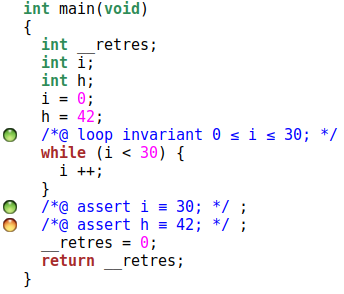
\includegraphics[scale=0.5]{3-3-boucle-effet-bord.png}
\caption{Encore des effets de bord}
\end{figure}

Il semble que non.

\subsection{\texorpdfstring{La clause \og{}assigns\fg{} \ldots{} pour les
boucles}{La clause assigns \ldots{} pour les boucles}}\label{la-clause-assigns-pour-les-boucles}

En fait, à propos des boucles, WP ne considère vraiment \emph{que} ce
que lui fournit l'utilisateur pour faire ses déductions. Et ici
l'invariant ne nous dit rien à propos de l'évolution de la valeur de
\texttt{h}. Nous pourrions signaler l'invariance de toute variable du
programme mais ce serait beaucoup d'efforts. ACSL nous propose plus
simplement d'ajouter des annotations \texttt{assigns} pour les boucles.
Toute autre variable est considérée invariante. Par exemple :

\begin{footnotesize}\begin{Shaded}
\begin{Highlighting}[]
\DataTypeTok{int} \NormalTok{main()\{}
  \DataTypeTok{int} \NormalTok{i = }\DecValTok{0}\NormalTok{;}
  \DataTypeTok{int} \NormalTok{h = }\DecValTok{42}\NormalTok{;}
  
  \CommentTok{/*@}
\CommentTok{    loop invariant 0 <= i <= 30;}
\CommentTok{    loop assigns i;}
\CommentTok{  */}
  \KeywordTok{while}\NormalTok{(i < }\DecValTok{30}\NormalTok{)\{}
    \NormalTok{++i;}
  \NormalTok{\}}
  \CommentTok{//@assert i == 30;}
  \CommentTok{//@assert h == 42;}
\NormalTok{\}}
\end{Highlighting}
\end{Shaded}\end{footnotesize}

Cette fois, nous pouvons établir la correction de la boucle. Par contre
rien ne nous prouve sa terminaison. L'invariant de boucle n'est pas
suffisant pour effectuer une telle preuve. Par exemple, dans notre
programme, si nous réécrivons la boucle comme ceci :

\begin{footnotesize}\begin{Shaded}
\begin{Highlighting}[]
\CommentTok{/*@}
\CommentTok{  loop invariant 0 <= i <= 30;}
\CommentTok{  loop assigns i;}
\CommentTok{*/}
\KeywordTok{while}\NormalTok{(i < }\DecValTok{30}\NormalTok{)\{}
   
\NormalTok{\}}
\end{Highlighting}
\end{Shaded}\end{footnotesize}

L'invariant est bien vérifié également, mais nous ne pourrons jamais
prouver que la boucle termine : elle est infinie.

\subsection{Preuve partielle et preuve totale - Variant de
boucle}\label{preuve-partielle-et-preuve-totale---variant-de-boucle}

En vérification déductive, il y a deux types de correction, la
correction partielle et la correction totale. Dans le premier cas, la
formulation est \og{}si la pré-condition est validée et \textbf{si} le
calcul termine, alors la post-condition est validée\fg{}. Dans le second
cas, \og{}si la pré-condition est validée, alors le calcul termine et la
post-condition est validée\fg{}. WP s'intéresse par défaut à de la preuve
partielle :

\begin{footnotesize}\begin{Shaded}
\begin{Highlighting}[]
\DataTypeTok{void} \NormalTok{foo()\{}
  \KeywordTok{while}\NormalTok{(}\DecValTok{1}\NormalTok{)\{\}}
  \CommentTok{//assert \textbackslash{}false;}
\NormalTok{\}}
\end{Highlighting}
\end{Shaded}\end{footnotesize}

Si nous demandons la vérification de ce code en activant le contrôle de
RTE, nous obtenons ceci :

\begin{figure}[htbp]
\centering
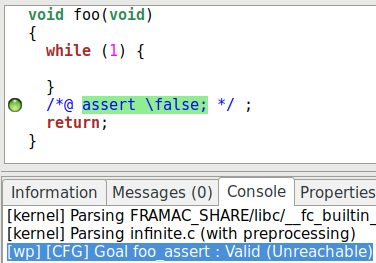
\includegraphics[scale=0.5]{3-3-infinite.png}
\caption{Preuve de faux par non-terminaison de boucle}
\end{figure}

L'assertion \og{}FAUX\fg{} est prouvée ! La raison est simple : la
non-terminaison de la boucle est triviale. Comme le calcul ne termine
pas et nous sommes en correction partielle, nous prouve ce que nous
voulons à la suite d'un calcul non terminant. Si la non-terminaison est
non-triviale, il y a peu de chances que l'assertion soit prouvée en
revanche.

\begin{zdsblock}{Information}
  À noter qu'une assertion
  inatteignable est toujours prouvée vraie de cette manière :
  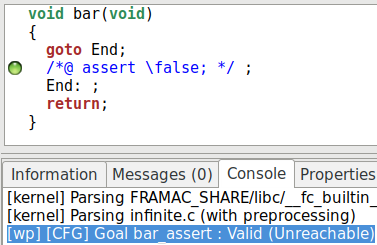
\includegraphics[scale=0.5]{3-3-goto_end.png}
  Et c'est également le cas lorsque l'on sait
  trivialement qu'une instruction produit nécessairement une
  erreur d'exécution (par exemple en déréférençant la valeur
  \texttt{NULL}), comme nous avions déjà pu le constater avec l'exemple
  de l'appel à \texttt{abs} avec la valeur \texttt{INT\_MIN}.
\end{zdsblock}

Pour prouver la terminaison d'une boucle, nous utilisons la notion de
variant de boucle. Le variant de boucle n'est pas une propriété mais une
valeur. C'est une expression faisant intervenir des éléments modifiés
par la boucle et donnant une borne supérieure sur le nombre d'itérations
restant à effectuer à un tour de la boucle. C'est donc une expression
supérieure à 0 et strictement décroissante d'un tour de boucle à l'autre
(cela sera également vérifié par induction par WP).

Si nous reprenons notre programme précédent, nous pouvons ajouter le
variant de cette façon :

\begin{footnotesize}\begin{Shaded}
\begin{Highlighting}[]
\DataTypeTok{int} \NormalTok{main()\{}
  \DataTypeTok{int} \NormalTok{i = }\DecValTok{0}\NormalTok{;}
  \DataTypeTok{int} \NormalTok{h = }\DecValTok{42}\NormalTok{;}
  
  \CommentTok{/*@}
\CommentTok{    loop invariant 0 <= i <= 30;}
\CommentTok{    loop assigns i;}
\CommentTok{    loop variant 30 - i;}
\CommentTok{  */}
  \KeywordTok{while}\NormalTok{(i < }\DecValTok{30}\NormalTok{)\{}
    \NormalTok{++i;}
  \NormalTok{\}}
  \CommentTok{//@assert i == 30;}
  \CommentTok{//@assert h == 42;}
\NormalTok{\}}
\end{Highlighting}
\end{Shaded}\end{footnotesize}

Une nouvelle fois nous pouvons regarder les buts générés :

\begin{figure}[htbp]
\centering
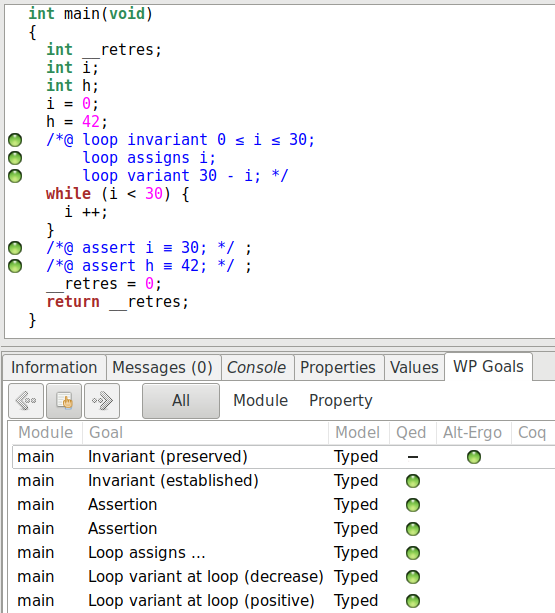
\includegraphics[scale=0.5]{3-3-boucle_complete.png}
\caption{Notre simple boucle complètement spécifiée et prouvée}
\end{figure}

Le variant nous génère bien deux obligations au niveau de la
vérification : assurer que la valeur est positive, et assurer qu'elle
décroît strictement pendant l'exécution de la boucle. Et si nous
supprimons la ligne de code qui incrémente \texttt{i}, WP ne peut plus
prouver que la valeur \texttt{30\ -\ i} décroît strictement.

\subsection{Lier la post-condition et
l'invariant}\label{lier-la-post-condition-et-linvariant}

Supposons le programme spécifié suivant. Notre but est de prouver que le
retour de cette fonction est l'ancienne valeur de \texttt{a} à laquelle
nous avons ajouté 10.

\begin{footnotesize}\begin{Shaded}
\begin{Highlighting}[]
\CommentTok{/*@}
\CommentTok{    ensures \textbackslash{}result == \textbackslash{}old(a) + 10;}
\CommentTok{*/}
\DataTypeTok{int} \NormalTok{plus_dix(}\DataTypeTok{int} \NormalTok{a)\{}
    \CommentTok{/*@}
\CommentTok{        loop invariant 0 <= i <= 10;}
\CommentTok{        loop assigns i, a;}
\CommentTok{        loop variant 10 - i;}
\CommentTok{    */}
    \KeywordTok{for} \NormalTok{(}\DataTypeTok{int} \NormalTok{i = }\DecValTok{0}\NormalTok{; i < }\DecValTok{10}\NormalTok{; ++i)}
        \NormalTok{++a;}

    \KeywordTok{return} \NormalTok{a;}
\NormalTok{\}}
\end{Highlighting}
\end{Shaded}\end{footnotesize}

Le calcul de plus faibles pré-conditions ne permet pas de sortir de la
boucle des informations qui ne font pas partie de l'invariant. Dans un
programme comme :

\begin{footnotesize}\begin{Shaded}
\begin{Highlighting}[]
\CommentTok{/*@}
\CommentTok{    ensures \textbackslash{}result == \textbackslash{}old(a) + 10;}
\CommentTok{*/}
\DataTypeTok{int} \NormalTok{plus_dix(}\DataTypeTok{int} \NormalTok{a)\{}
    \NormalTok{++a;}
    \NormalTok{++a;}
    \NormalTok{++a;}
    \CommentTok{//...}
    \KeywordTok{return} \NormalTok{a;}
\NormalTok{\}}
\end{Highlighting}
\end{Shaded}\end{footnotesize}

En remontant les instructions depuis la post-condition, on conserve
toujours les informations à propos de \texttt{a}. À l'inverse, comme
mentionné plus tôt, en dehors de la boucle WP ne considérera que les
connaissances fournies par notre invariant. Par conséquent, notre
fonction \texttt{plus\_dix} ne peut pas être prouvée en l'état :
l'invariant ne mentionne aucune connaissance à propos de \texttt{a}.
Pour lier notre post-condition à l'invariant, il faut ajouter une telle
connaissance. Par exemple :

\begin{footnotesize}\begin{Shaded}
\begin{Highlighting}[]
\CommentTok{/*@}
\CommentTok{    ensures \textbackslash{}result == \textbackslash{}old(a) + 10;}
\CommentTok{*/}
\DataTypeTok{int} \NormalTok{plus_dix(}\DataTypeTok{int} \NormalTok{a)\{}
    \CommentTok{/*@}
\CommentTok{        loop invariant 0 <= i <= 10;}
\CommentTok{        loop invariant a = \textbackslash{}old(a) + i; //< AJOUT}
\CommentTok{        loop assigns i, a;}
\CommentTok{        loop variant 10 - i;}
\CommentTok{    */}
    \KeywordTok{for} \NormalTok{(}\DataTypeTok{int} \NormalTok{i = }\DecValTok{0}\NormalTok{; i < }\DecValTok{10}\NormalTok{; ++i)}
        \NormalTok{++a;}

    \KeywordTok{return} \NormalTok{a;}
\NormalTok{\}}
\end{Highlighting}
\end{Shaded}\end{footnotesize}

\begin{zdsblock}
  Ce besoin peut semble être une
  contrainte très forte. Elle ne l'est en fait pas tant que
  cela. Il existe des analyses fortement automatiques capables de
  calculer les invariants de boucles. Par exemple, sans
  spécifications, une interprétation abstraite calculera assez
  facilement \texttt{0\ \textless{}=\ i\ \textless{}=\ 10} et 
  \texttt{\textbackslash{}old(a)\ \textless{}=\ a\ \textless{}=\ \textbackslash{}old(a)+10}.
  En revanche, il est souvent bien plus difficile de calculer
  les relations qui existent entre des variables différentes qui
  évoluent dans le même programme, par exemple l'égalité
  mentionnée par notre invariant ajouté.
\end{zdsblock}

\section{Les boucles - Exemples}\label{les-boucles---exemples}

\subsection{Exemple avec un tableau
read-only}\label{exemple-avec-un-tableau-read-only}

S'il y a une structure de données que nous traitons avec les boucles
c'est bien le tableau. C'est une bonne base d'exemples pour les boucles
car ils permettent rapidement de présenter des invariants intéressants
et surtout, il va permettre d'introduire des constructions très
importantes d'ACSL.

Prenons par exemple la fonction qui cherche une valeur dans un tableau :

\begin{footnotesize}\begin{Shaded}
\begin{Highlighting}[]
\CommentTok{#include <stddef.h>}

\CommentTok{/*@}
\CommentTok{  requires 0 < length;}
\CommentTok{  requires \textbackslash{}valid_read(array + (0 .. length-1));}
\CommentTok{  }
\CommentTok{  assigns  \textbackslash{}nothing;}

\CommentTok{  behavior in:}
\CommentTok{    assumes \textbackslash{}exists size_t off ; 0 <= off < length && array[off] == element;}
\CommentTok{    ensures array <= \textbackslash{}result < array+length && *\textbackslash{}result == element;}

\CommentTok{  behavior notin:}
\CommentTok{    assumes \textbackslash{}forall size_t off ; 0 <= off < length ==> array[off] != element;}
\CommentTok{    ensures \textbackslash{}result == NULL;}

\CommentTok{  disjoint behaviors;}
\CommentTok{  complete behaviors;}
\CommentTok{*/}
\DataTypeTok{int}\NormalTok{* search(}\DataTypeTok{int}\NormalTok{* array, size_t length, }\DataTypeTok{int} \NormalTok{element)\{}
  \CommentTok{/*@}
\CommentTok{    loop invariant 0 <= i <= length;}
\CommentTok{    loop invariant \textbackslash{}forall size_t j; 0 <= j < i ==> array[j] != element;}
\CommentTok{    loop assigns i;}
\CommentTok{    loop variant length-i;}
\CommentTok{  */} 
  \KeywordTok{for}\NormalTok{(size_t i = }\DecValTok{0}\NormalTok{; i < length; i++)}
    \KeywordTok{if}\NormalTok{(array[i] == element) }\KeywordTok{return} \NormalTok{&array[i];}
  \KeywordTok{return} \NormalTok{NULL;}
\NormalTok{\}}
\end{Highlighting}
\end{Shaded}\end{footnotesize}

Cet exemple est suffisamment fourni pour introduire des notations
importantes.

D'abord, comme nous l'avons déjà mentionné, le prédicat
\texttt{\textbackslash{}valid\_read} (de même que
\texttt{\textbackslash{}valid}) nous permet de spécifier non seulement
la validité d'une adresse en lecture mais également celle de tout un
ensemble d'adresses contiguës. C'est la notation que nous avons utilisée
dans cette expression :

\begin{footnotesize}\begin{Shaded}
\begin{Highlighting}[]
\CommentTok{//@ requires \textbackslash{}valid_read(a + (0 .. length-1));}
\end{Highlighting}
\end{Shaded}\end{footnotesize}

Cette pré-condition nous atteste que les adresses a+0, a+1 \ldots{},
a+length-1 sont valides en lecture.

Nous avons également introduit deux notations qui vont nous être très
utiles, à savoir \texttt{\textbackslash{}forall} (\(\forall\)) et
\texttt{\textbackslash{}exists} (\(\exists\)), les quantificateurs de la
logique. Le premier nous servant à annoncer que pour tout élément, la
propriété suivante est vraie. Le second pour annoncer qu'il existe un
élément tel que la propriété est vraie. Si nous commentons les deux
lignes en questions, nous pouvons les lire de cette façon :

\begin{footnotesize}\begin{Shaded}
\begin{Highlighting}[]
\CommentTok{/*@}
\CommentTok{//pour tout "off" de type "size_t", tel que SI "off" est compris entre 0 et "length"}
\CommentTok{//                                 ALORS la case "off" de "a" est différente de "element"}
\CommentTok{\textbackslash{}forall size_t off ; 0 <= off < length ==> a[off] != element;}

\CommentTok{//il existe "off" de type "size_t", tel que "off" soit compris entre 0 et "length"}
\CommentTok{//                                 ET que la case "off" de "a" vaille "element"}
\CommentTok{\textbackslash{}exists size_t off ; 0 <= off < length && a[off] == element;}
\CommentTok{*/}
\end{Highlighting}
\end{Shaded}\end{footnotesize}

Si nous devions résumer leur utilisation, nous voudrions dire que sur un
certain ensemble d'éléments, une propriété est vraie, soit à propos d'au
moins l'un d'eux, soit à propos de la totalité d'entre eux. Un schéma
qui reviendra typiquement dans ce cas est que nous restreindrons cet
ensemble à travers une première propriété (ici :
\texttt{0\ \textless{}=\ off\ \textless{}\ length}) puis nous voudrons
prouver la propriété réelle qui nous intéresse à propos d'eux.
\textbf{Mais il y a une différence fondamentale entre l'usage de
\texttt{exists} et celui de \texttt{forall}}.

Avec
\texttt{\textbackslash{}forall\ type\ a\ ;\ p(a)\ ==\textgreater{}\ q(a)},
la restriction (\texttt{p}) est suivie par une implication. Pour tout
élément, s'il respecte une première propriété (\texttt{p}), alors
vérifier la seconde propriété \texttt{q}. Si nous mettions un ET comme
pour le \og{}il existe\fg{} que nous expliquerons ensuite, cela voudrait dire
que nous voulons que tout élément respecte à la fois les deux
propriétés. Parfois, cela peut être ce que nous voulons exprimer, mais
cela ne correspond alors plus à l'idée de restreindre un ensemble dont
nous voulons montrer une propriété particulière.

Avec \texttt{\textbackslash{}exists\ type\ a\ ;\ p(a)\ \&\&\ q(a)}, la
restriction (\texttt{p}) est suivie par une conjonction, nous voulons
qu'il existe un élément tel que cet élément est dans un certain état
(défini par \texttt{p}), tout en respectant l'autre propriété
\texttt{q}. Si nous mettions une implication comme pour le \og{}pour
tout\fg{}, alors une telle expression devient toujours vraie à moins que p
soit une tautologie ! Pourquoi ? Existe-t-il \og{}a\fg{} tel que p(a) implique
q(a) ? Prenons n'importe quel \og{}a\fg{} tel que p(a) est faux, l'implication
devient vraie.

Cette partie de l'invariant mérite une attention particulière :

\begin{footnotesize}\begin{Shaded}
\begin{Highlighting}[]
\CommentTok{//@ loop invariant \textbackslash{}forall size_t j; 0 <= j < i ==> array[j] != element;}
\end{Highlighting}
\end{Shaded}\end{footnotesize}

En effet, c'est la partie qui définit l'action de notre boucle, elle
indique à WP ce que la boucle va faire (ou apprendre dans le cas
présent) tout au long de son exécution. Ici en l'occurrence, cet formule
nous dit qu'à chaque tour, nous savons que pour toute case entre 0 et la
prochaine que nous allons visiter \texttt{i} (exclue), elle stocke une
valeur différente de l'élément recherché.

Le but WP associé à la préservation de cet invariant est un peu
compliqué, il n'est pour nous pas très intéressant de se pencher dessus.
En revanche, la preuve de l'établissement de cet invariant est
intéressante :

\begin{figure}[htbp]
\centering
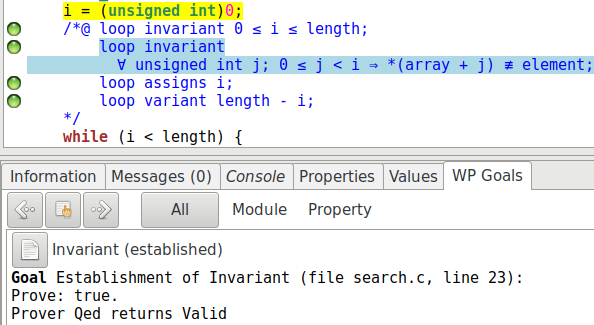
\includegraphics[scale=0.5]{3-4-trivial-establishment.png}
\caption{But trivial}
\end{figure}

Nous pouvons constater que cette propriété, pourtant complexe, est
prouvée par Qed sans aucun problème. Si nous regardons sur quelles
parties du programme la preuve se base, nous pouvons voir l'instruction
\texttt{i\ =\ 0} surlignée, et c'est bien la dernière instruction que
nous effectuons sur \texttt{i} avant de commencer la boucle. Et donc
effectivement, si nous faisons le remplacement dans la formule de
l'invariant :

\begin{footnotesize}\begin{Shaded}
\begin{Highlighting}[]
\CommentTok{//@ loop invariant \textbackslash{}forall size_t j; 0 <= j < 0 ==> array[j] != element;}
\end{Highlighting}
\end{Shaded}\end{footnotesize}

\og{}Pour tout j, supérieur ou égal à 0 et inférieur strict à 0\fg{}, cette
partie est nécessairement fausse. Notre implication est nécessairement
vraie.

\subsection{Exemples avec tableaux
mutables}\label{exemples-avec-tableaux-mutables}

Nous allons voir deux exemples avec la manipulation de tableaux en
mutation. L'un avec une modification totale, l'autre en modification
sélective.

\subsubsection{Remise à zéro}\label{remise-uxe0-zuxe9ro}

Regardons la fonction effectuant la remise à zéro d'un tableau.

\begin{footnotesize}\begin{Shaded}
\begin{Highlighting}[]
\CommentTok{#include <stddef.h>}

\CommentTok{/*@}
\CommentTok{  requires \textbackslash{}valid(array + (0 .. length-1));}
\CommentTok{  assigns  array[0 .. length-1];}
\CommentTok{  ensures  \textbackslash{}forall size_t i; 0 <= i < length ==> array[i] == 0;}
\CommentTok{*/}
\DataTypeTok{void} \NormalTok{raz(}\DataTypeTok{int}\NormalTok{* array, size_t length)\{}
  \CommentTok{/*@}
\CommentTok{    loop invariant 0 <= i <= length;}
\CommentTok{    loop invariant \textbackslash{}forall size_t j; 0 <= j < i ==> array[j] == 0;}
\CommentTok{    loop assigns i, array[0 .. length-1];}
\CommentTok{    loop variant length-i;}
\CommentTok{  */}
  \KeywordTok{for}\NormalTok{(size_t i = }\DecValTok{0}\NormalTok{; i < length; ++i)}
    \NormalTok{array[i] = }\DecValTok{0}\NormalTok{;}
\NormalTok{\}}
\end{Highlighting}
\end{Shaded}\end{footnotesize}

Les seules parties sur lesquelles nous pouvons nous attacher ici sont
les \texttt{assigns} de la fonction et de la boucle. À nouveau, nous
pouvons utiliser a notation \texttt{n\ ..\ m} pour indiquer les parties
du tableau qui sont modifiées.

\subsubsection{Chercher et remplacer}\label{chercher-et-remplacer}

Le dernier exemple qui nous intéresse est l'algorithme chercher et
remplacer. C'est donc un algorithme qui va sélectivement modifier des
valeurs dans une certaine plage d'adresses. Il est toujours un peu
difficile de guider l'outil dans ce genre de cas car nous devons garder
\og{}en mémoire\fg{}, ce qui est modifié et ce qui ne l'est pas et que
l'induction repose sur ce fait.

À titre d'exemple, la première spécification que nous pouvons réaliser
pour cette fonction ressemblerait à ceci :

\begin{footnotesize}\begin{Shaded}
\begin{Highlighting}[]
\CommentTok{#include <stddef.h>}

\CommentTok{/*@}
\CommentTok{  requires \textbackslash{}valid(array + (0 .. length-1));}
\CommentTok{  assigns array[0 .. length-1];}

\CommentTok{  ensures \textbackslash{}forall size_t i; 0 <= i < length && \textbackslash{}old(array[i]) == old}
\CommentTok{             ==> array[i] == new;}
\CommentTok{  ensures \textbackslash{}forall size_t i; 0 <= i < length && \textbackslash{}old(array[i]) != old }
\CommentTok{             ==> array[i] == \textbackslash{}old(array[i]);}
\CommentTok{*/}
\DataTypeTok{void} \NormalTok{search_and_replace(}\DataTypeTok{int}\NormalTok{* array, size_t length, }\DataTypeTok{int} \NormalTok{old, }\DataTypeTok{int} \NormalTok{new)\{}
  \CommentTok{/*@}
\CommentTok{    loop invariant 0 <= i <= length;}
\CommentTok{    loop invariant \textbackslash{}forall size_t j; 0 <= j < i && \textbackslash{}at(array[j], Pre) == old }
\CommentTok{                     ==> array[j] == new;}
\CommentTok{    loop invariant \textbackslash{}forall size_t j; 0 <= j < i && \textbackslash{}at(array[j], Pre) != old }
\CommentTok{                     ==> array[j] == \textbackslash{}at(array[j], Pre);}
\CommentTok{    loop assigns i, array[0 .. length-1];}
\CommentTok{    loop variant length-i;}
\CommentTok{  */}
  \KeywordTok{for}\NormalTok{(size_t i = }\DecValTok{0}\NormalTok{; i < length; ++i)\{}
    \KeywordTok{if}\NormalTok{(array[i] == old) array[i] = new;}
  \NormalTok{\}}
\NormalTok{\}}
\end{Highlighting}
\end{Shaded}\end{footnotesize}

Nous utilisons la fonction logique \texttt{\textbackslash{}at} dont nous
avons déjà expliqué le fonctionnement plus tôt. Si nous regardons
l'utilisation qui en est faite ici, nous voyons que dans l'invariant de
boucle, nous cherchons à établir une relation entre les anciennes
valeurs du tableau et leurs potentielles nouvelles valeurs :

\begin{footnotesize}\begin{Shaded}
\begin{Highlighting}[]
\CommentTok{/*@}
\CommentTok{  loop invariant \textbackslash{}forall size_t j; 0 <= j < i && \textbackslash{}at(array[j], Pre) == old }
\CommentTok{                   ==> array[j] == new;}
\CommentTok{  loop invariant \textbackslash{}forall size_t j; 0 <= j < i && \textbackslash{}at(array[j], Pre) != old }
\CommentTok{                   ==> array[j] == \textbackslash{}at(array[j], Pre);}
\CommentTok{*/}
\end{Highlighting}
\end{Shaded}\end{footnotesize}

Pour tout élément que nous avons visité, s'il valait la valeur qui doit
être remplacée, alors il vaut la nouvelle valeur, sinon il n'a pas
changé. En fait si nous essayons de prouver l'invariant, WP n'y parvient
pas. Dans ce genre de cas, le plus simple est encore d'ajouter diverses
assertions exprimant les propriétés intermédiaires que nous nous
attendons à voir facilement prouvées et impliquant l'invariant. En fait,
nous nous apercevons rapidement que WP n'arrive pas à maintenir le fait
que nous n'avons pas encore modifié la fin du tableau :

\begin{footnotesize}\begin{Shaded}
\begin{Highlighting}[]
\KeywordTok{for}\NormalTok{(size_t i = }\DecValTok{0}\NormalTok{; i < length; ++i)\{}
    \CommentTok{//@assert array[i] == \textbackslash{}at(array[i], Pre); // échec de preuve}
    \KeywordTok{if}\NormalTok{(array[i] == old) array[i] = new;}
\NormalTok{\}}
\end{Highlighting}
\end{Shaded}\end{footnotesize}

Nous pouvons donc ajouter cette information comme invariant :

\begin{footnotesize}\begin{Shaded}
\begin{Highlighting}[]
\CommentTok{/*@}
\CommentTok{  loop invariant 0 <= i <= length;}
\CommentTok{  loop invariant \textbackslash{}forall size_t j; 0 <= j < i && \textbackslash{}at(array[j], Pre) == old }
\CommentTok{                   ==> array[j] == new;}
\CommentTok{  loop invariant \textbackslash{}forall size_t j; 0 <= j < i && \textbackslash{}at(array[j], Pre) != old }
\CommentTok{                   ==> array[j] == \textbackslash{}at(array[j], Pre);}

\CommentTok{  //La fin du tableau n'a pas été modifiée :}
\CommentTok{  loop invariant \textbackslash{}forall size_t j; i <= j < length}
\CommentTok{                     ==> array[j] == \textbackslash{}at(array[j], Pre);}
\CommentTok{  loop assigns i, array[0 .. length-1];}
\CommentTok{  loop variant length-i;}
\CommentTok{*/}
\KeywordTok{for}\NormalTok{(size_t i = }\DecValTok{0}\NormalTok{; i < length; ++i)\{}
  \KeywordTok{if}\NormalTok{(array[i] == old) array[i] = new;}
\NormalTok{\}}
\end{Highlighting}
\end{Shaded}\end{footnotesize}

Et cette fois, la preuve passera. À noter que si nous tentons la preuve
directement avec la vérification des RTE, il est possible qu'Alt-Ergo
n'y parvienne pas (CVC4 décharge l'ensemble sans problème). Dans ce cas,
nous pouvons faire séparément les deux preuves (sans, puis avec RTE) ou
encore ajouter des assertions permettant de guider la preuve dans la
boucle :

\begin{footnotesize}\begin{Shaded}
\begin{Highlighting}[]
\KeywordTok{for}\NormalTok{(size_t i = }\DecValTok{0}\NormalTok{; i < length; ++i)\{}
  \KeywordTok{if}\NormalTok{(array[i] == old) array[i] = new;}

  \CommentTok{/*@ assert \textbackslash{}forall size_t j; i < j < length }
\CommentTok{               ==> array[j] == \textbackslash{}at(array[j], Pre);                      */}
  \CommentTok{/*@ assert \textbackslash{}forall size_t j; 0 <= j <= i && \textbackslash{}at(array[j], Pre) == old }
\CommentTok{               ==> array[j] == new;                                     */}
  \CommentTok{/*@ assert \textbackslash{}forall size_t j; 0 <= j <= i && \textbackslash{}at(array[j], Pre) != old }
\CommentTok{               ==> array[j] == \textbackslash{}at(array[j], Pre);                      */}    
\NormalTok{\}}
\end{Highlighting}
\end{Shaded}\end{footnotesize}

À mesure que nous cherchons à prouver des propriétés plus compliquées et
notamment dépendantes de boucles, il va y avoir une part de tâtonnement
pour comprendre ce qui manque au prouveur pour réussir la preuve.

Ce qui peut lui manquer, c'est des hypothèses. Dans ce type de cas, nous
pouvons tenter d'ajouter des assertions au code pour guider le prouveur.
Avec de l'expérience, nous pouvons regarder le contenu des obligations
de preuve ou tenter de commencer la preuve avec Coq pour voir si la
preuve semble réalisable. Parfois le prouveur manque juste de temps,
auquel cas, il suffit d'augmenter (parfois beaucoup) la durée du
timeout. Finalement, la propriété peut également être hors de portée du
prouveur. Auquel cas, il faudra écrire une preuve à la main avec un
prouveur interactif.

Enfin, il reste le cas où l'implémentation est effectivement fausse, et
dans ce cas, il faut la corriger. Et c'est là que nous utiliserons
plutôt le test que la preuve, car le test permet de prouver la présence
d'un bug ;) .

Dans cette partie nous avons pu voir comment se traduisent les
affectations et les structures de contrôle d'un point de vue logique.
Nous nous sommes beaucoup attardés sur les boucles parce que c'est là
que se trouvent la majorité des difficultés lorsque nous voulons
spécifier et prouver un programme par vérification déductive, les
annotations ACSL qui leur sont spécifiques nous permettent d'exprimer le
plus précisément possible leur comportement.

Pour la suite, nous allons nous attarder plus précisément sur les
constructions que nous offre le langage ACSL du côté de la logique.
Elles sont très importantes parce que ce sont elles qui vont nous
permettre de nous abstraire du code pour avoir des spécifications plus
compréhensibles et plus aisément prouvables.

\chapter{ACSL - Propriétés}\label{acsl---propriuxe9tuxe9s}

Depuis le début de ce tutoriel, nous avons vu divers prédicats et
fonctions logiques qui sont fournis par défaut en ACSL :
\texttt{\textbackslash{}valid}, \texttt{\textbackslash{}valid\_read},
\texttt{\textbackslash{}separated}, \texttt{\textbackslash{}old} et
\texttt{\textbackslash{}at}. Il en existe bien sûr d'autres mais nous
n'allons pas les présenter un à un, le lecteur pourra se référer à
\href{http://frama-c.com/download.html}{la documentation (ACSL
implementation)} pour cela (à noter : tout n'est pas nécessairement
supporté par WP).

ACSL nous permet de faire plus que \og{}simplement\fg{} spécifier notre code.
Nous pouvons définir nos propres prédicats, fonctions, relations, etc.
Le but est de pouvoir abstraire nos spécifications. Cela nous permet de
les factoriser (par exemple en définissant ce qu'est un tableau valide),
ce qui a deux effets positifs pour nous : d'abord nos spécifications
deviennent plus lisibles donc plus faciles à comprendre, mais cela
permet également de réutiliser des preuves déjà faites et donc de
faciliter la preuve de nouveaux programmes.

\section{Types primitifs
supplémentaires}\label{types-primitifs-suppluxe9mentaires}

ACSL nous propose deux types qui vont permettre d'être d'écrire des
propriétés ou des fonctions sans avoir à se préoccuper des contraintes
dues à la taille en mémoire des types primitifs du C. Ces types sont
\texttt{integer} et \texttt{real}. Qui représente respectivement les
vrais entiers et les \og{}aussi vrai que possible\fg{} réels.

Par la suite, nous utiliserons souvent des entiers à la place des
classiques \texttt{ìnt} du C. La raison est simplement que beaucoup de
propriété sont vraies quelle que soit la taille de l'entier (au sens C,
cette fois) en entrée.

En revanche, nous ne parlerons pas de \texttt{real} VS
\texttt{float/double}, parce que cela induirait que nous parlions de
preuve de programmes avec du calcul en virgule flottante. Et nous ne
parlerons pas de preuve de programmes impliquant du calcul en virgule
flottante. Par contre, ce tutoriel en cours d'écriture en parle :
\href{https://zestedesavoir.com/forums/sujet/4157/effectuer-des-calculs-numeriques-precis/}{Effectuer
des calculs numériques précis}.

\section{Prédicats}\label{pruxe9dicats}

Un prédicat est une propriété portant sur des objets et pouvant être
vraie ou fausse. En résumé, des prédicats, c'est ce que nous écrivons
depuis le début de ce tutoriel dans les clauses de nos contrats et de
nos invariants de boucle. ACSL nous permet de créer des versions nommées
de ces prédicats, à la manière d'une fonction booléenne en C par
exemple. À la différence près tout de même que les prédicats (ainsi que
les fonctions logiques que nous verrons par la suite) doivent être
pures, c'est-à-dire qu'elles ne peuvent pas produire d'effets de bords
en modifiant des valeurs pointées par exemple.

Ces prédicats peuvent prendre un certain nombre de paramètres. En plus
de cela, ils peuvent également recevoir un certain nombre de labels (au
sens C du terme) qui vont permettre d'établir des relations entre divers
points du code.

\subsection{Syntaxe}\label{syntaxe}

Les prédicats sont, comme les spécifications, introduits au travers
d'annotations. La syntaxe est la suivante :

\begin{footnotesize}\begin{Shaded}
\begin{Highlighting}[]
\CommentTok{/*@}
\CommentTok{  predicate nom_du_predicat \{ Label0, Label1, ..., LabelN \}(type0 arg0, type1 arg1, ..., typeN argN) =}
\CommentTok{    //une relation logique entre toutes ces choses.}
\CommentTok{*/}
\end{Highlighting}
\end{Shaded}\end{footnotesize}

Nous pouvons par exemple définir le prédicat nous disant qu'un entier en
mémoire n'a pas changé entre deux points particuliers de programme :

\begin{footnotesize}\begin{Shaded}
\begin{Highlighting}[]
\CommentTok{/*@}
\CommentTok{  predicate unchanged\{L0, L1\}(int* i) =}
\CommentTok{    \textbackslash{}at(*i, L0) == \textbackslash{}at(*i, L1);}
\CommentTok{*/}
\end{Highlighting}
\end{Shaded}\end{footnotesize}

\begin{zdsalertblock}{Attention}
  Gardez bien en mémoire que le passage
  se fait, comme en C, par valeur. Nous ne pouvons pas écrire
  ce prédicat en passant directement \texttt{i} :
  \begin{footnotesize}\begin{Shaded}
    \begin{Highlighting}[]
\CommentTokAlt{/*@}
\CommentTokAlt{  predicate unchanged\{L0, L1\}(int i) =}
\CommentTokAlt{    \textbackslash{}at(i, L0) == \textbackslash{}at(i, L1);}
\CommentTokAlt{*/}
    \end{Highlighting}
  \end{Shaded}\end{footnotesize}
  Car i est juste une copie de la variable reçue en paramètre.
\end{zdsalertblock}
  
Nous pouvons par exemple vérifier ce petit code :

\begin{footnotesize}\begin{Shaded}
\begin{Highlighting}[]
\DataTypeTok{int} \NormalTok{main()\{}
  \DataTypeTok{int} \NormalTok{i = }\DecValTok{13}\NormalTok{;}
  \DataTypeTok{int} \NormalTok{j = }\DecValTok{37}\NormalTok{;}

 \NormalTok{Begin:}
  \NormalTok{i = }\DecValTok{23}\NormalTok{;}
 
  \CommentTok{//@assert ! unchanged\{Begin, Here\}(&i);}
  \CommentTok{//@assert   unchanged\{Begin, Here\}(&j);}
\NormalTok{\}}
\end{Highlighting}
\end{Shaded}\end{footnotesize}

Nous pouvons également regarder les buts générés par WP et constater
que, même s'il subit une petite transformation syntaxique, le prédicat
n'est pas déroulé par WP. Ce sera au prouveur de déterminer s'il veut
raisonner avec.

Comme nous l'avons dit plus tôt, une des utilités des prédicats et
fonctions (que nous verrons un peu plus tard) est de rendre plus lisible
nos spécification et de les factoriser. Un exemple est d'écrire un
prédicat pour la validité en lecture/écriture d'un tableau sur une plage
particulière. Cela nous évite d'avoir à réécrire l'expression en
question qui est moins compréhensible au premier coup d'œil.

\begin{footnotesize}\begin{Shaded}
\begin{Highlighting}[]
\CommentTok{/*@}
\CommentTok{  predicate valid_range_rw(int* t, integer n) =}
\CommentTok{    n >= 0 && \textbackslash{}valid(t + (0 .. n-1));}

\CommentTok{  predicate valid_range_ro(int* t, integer n) =}
\CommentTok{    n >= 0 && \textbackslash{}valid_read(t + (0 .. n-1));}
\CommentTok{*/}

\CommentTok{/*@}
\CommentTok{  requires 0 < length;}
\CommentTok{  requires valid_range_ro(array, length);}
\CommentTok{  //...}
\CommentTok{*/}
\DataTypeTok{int}\NormalTok{* search(}\DataTypeTok{int}\NormalTok{* array, size_t length, }\DataTypeTok{int} \NormalTok{element)}
\end{Highlighting}
\end{Shaded}\end{footnotesize}

Dans cette portion de spécification, le label pour les prédicats n'est
pas précisé, ni pour leur création, ni pour leur utilisation. Pour la
création, Frama-C va automatiquement en ajouter un dans la définition du
prédicat. Pour l'appel, le label passé sera implicitement \texttt{Here}.
La non-déclaration du label dans la définition n'interdit pour autant
pas de passer explicitement un label lors de l'appel.

Bien entendu, les prédicats peuvent être déclarés dans des fichiers
headers afin de produire une bibliothèque d'utilitaires de
spécifications par exemple.

\subsection{Abstraction}\label{abstraction}

Une autre utilité importante des prédicats est de définir l'état logique
de nos structures quand les programmes se complexifient. Nos structures
doivent généralement respecter un invariant (encore) que chaque fonction
de manipulation devra maintenir pour assurer que la structure sera
toujours utilisable et qu'aucune fonction ne commettra de bavure.

Cela permet notamment de faciliter la lecture de spécifications. Par
exemple, nous pourrions poser les spécifications nécessaires à la sûreté
d'une pile de taille limitée. Et cela donnerait quelque chose comme :

\begin{footnotesize}\begin{Shaded}
\begin{Highlighting}[]
\KeywordTok{struct} \NormalTok{stack_int\{}
  \NormalTok{size_t top;}
  \DataTypeTok{int}    \NormalTok{data[MAX_SIZE];}
\NormalTok{\};}

\CommentTok{/*@}
\CommentTok{  predicate valid_stack_int(struct stack_int* s) = // à définir ;}
\CommentTok{  predicate empty_stack_int(struct stack_int* s) = // à définir ;}
\CommentTok{  predicate full_stack_int(struct stack_int* s) =  // à définir ;}
\CommentTok{*/}

\CommentTok{/*@}
\CommentTok{  requires \textbackslash{}valid(s);}
\CommentTok{  assigns *s;}
\CommentTok{  ensures valid_stack_int(s) && empty_stack_int(s);}
\CommentTok{*/}
\DataTypeTok{void} \NormalTok{initialize(}\KeywordTok{struct} \NormalTok{stack_int* s);}

\CommentTok{/*@}
\CommentTok{  requires valid_stack_int(s) && !full_stack_int(s);}
\CommentTok{  assigns  *s;}
\CommentTok{  ensures valid_stack_int(s);}
\CommentTok{*/}
\DataTypeTok{void} \NormalTok{push(}\KeywordTok{struct} \NormalTok{stack_int* s, }\DataTypeTok{int} \NormalTok{value);}

\CommentTok{/*@}
\CommentTok{  requires valid_stack_int(s) && !empty_stack_int(s);}
\CommentTok{  assigns \textbackslash{}nothing;}
\CommentTok{*/}
\DataTypeTok{int}  \NormalTok{top(}\KeywordTok{struct} \NormalTok{stack_int* s);}

\CommentTok{/*@}
\CommentTok{  requires valid_stack_int(s) && !empty_stack_int(s);}
\CommentTok{  assigns *s;}
\CommentTok{  ensures valid_stack_int(s);}
\CommentTok{*/}
\DataTypeTok{void} \NormalTok{pop(}\KeywordTok{struct} \NormalTok{stack_int* s);}

\CommentTok{/*@}
\CommentTok{  requires valid_stack_int(s);}
\CommentTok{  assigns \textbackslash{}nothing;}
\CommentTok{  ensures \textbackslash{}result == 1 <==> empty_stack_int(s);}
\CommentTok{*/}
\DataTypeTok{int}  \NormalTok{is_empty(stack_int_t s);}


\CommentTok{/*@}
\CommentTok{  requires valid_stack_int(s);}
\CommentTok{  assigns \textbackslash{}nothing;}
\CommentTok{  ensures \textbackslash{}result == 1 <==> full_stack_int(s);}
\CommentTok{*/}
\DataTypeTok{int}  \NormalTok{is_full(stack_int_t s);}
\end{Highlighting}
\end{Shaded}\end{footnotesize}

Ici la spécification n'exprime pas de propriétés fonctionnelles. Par
exemple, rien ne nous spécifie que lorsque nous faisons un push une
valeur puis que nous demandons top, nous auront effectivement cette
valeur. Mais elle nous donne déjà tout ce dont nous avons besoin pour
produire un code où à défaut d'avoir exactement les résultats que nous
attendons, nous ne pouvons pas avoir d'erreur d'exécution (à condition
de poser une spécification correcte pour nos prédicats et de prouver les
fonctions d'utilisation de la structure).

\section{Fonctions logiques}\label{fonctions-logiques}

Les fonctions logiques nous permettent de décrire des fonctions qui ne
seront utilisables que dans les spécifications. Cela nous permet, d'une
part, de les factoriser, et d'autre part de définir des opérations sur
les types integer et real qui ne peuvent pas déborder contrairement aux
types machines.

Comme les prédicats, elles peuvent recevoir divers labels et valeurs en
paramètre.

\subsection{Syntaxe}\label{syntaxe-1}

Pour déclarer une fonction logique, l'écriture est la suivante :

\begin{footnotesize}\begin{Shaded}
\begin{Highlighting}[]
\CommentTok{/*@}
\CommentTok{  logic type_retour ma_fonction\{ Label0, ..., LabelN \}( type0 arg0, ..., typeN argN ) =}
\CommentTok{    formule mettant en jeu les arguments ;}
\CommentTok{*/}
\end{Highlighting}
\end{Shaded}\end{footnotesize}

Nous pouvons par exemple décrire une fonction affine générale du côté de
la logique :

\begin{footnotesize}\begin{Shaded}
\begin{Highlighting}[]
\CommentTok{/*@}
\CommentTok{  logic integer ax_b(integer a, integer x, integer b) =}
\CommentTok{    a * x + b;}
\CommentTok{*/}
\end{Highlighting}
\end{Shaded}\end{footnotesize}

Elle peut nous servir à prouver le code de la fonction suivante :

\begin{footnotesize}\begin{Shaded}
\begin{Highlighting}[]
\CommentTok{/*@ }
\CommentTok{  assigns \textbackslash{}nothing ;}
\CommentTok{  ensures \textbackslash{}result == ax_b(3,x,4); }
\CommentTok{*/}
\DataTypeTok{int} \NormalTok{function(}\DataTypeTok{int} \NormalTok{x)\{}
  \KeywordTok{return} \DecValTok{3}\NormalTok{*x + }\DecValTok{4}\NormalTok{;}
\NormalTok{\}}
\end{Highlighting}
\end{Shaded}\end{footnotesize}

\begin{figure}[htbp]
\centering
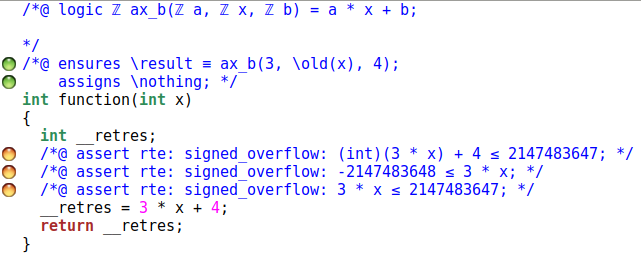
\includegraphics[scale=0.5]{4-3-affine-1.png}
\caption{Les débordements semblent pouvoir survenir}
\end{figure}

Le code est bien prouvé mais les contrôles d'overflow, eux, ne le sont
pas. Nous pouvons à nouveau définir des fonctions logiques générales
pour avoir les bornes calculées de côté de la logique en fonction des
valeurs que nous donnons en entrée. Ainsi qu'ajouter nos contrôles de
bornes en pré-condition de fonction :

\begin{footnotesize}\begin{Shaded}
\begin{Highlighting}[]
\CommentTok{/*@}
\CommentTok{  logic integer limit_int_min_ax_b(integer a, integer b) =}
\CommentTok{    (a == 0) ? (b > 0) ? INT_MIN : INT_MIN-b :}
\CommentTok{    (a <  0) ? (INT_MAX-b)/a :}
\CommentTok{               (INT_MIN-b)/a ;}

\CommentTok{  logic integer limit_int_max_ax_b(integer a, integer b) =}
\CommentTok{    (a == 0) ? (b > 0) ? INT_MAX-b : INT_MAX :}
\CommentTok{    (a <  0) ? (INT_MIN-b)/a :}
\CommentTok{               (INT_MAX-b)/a ;}
\CommentTok{*/}

\CommentTok{/*@}
\CommentTok{  requires limit_int_min_ax_b(3,4) < x < limit_int_max_ax_b(3,4);}
\CommentTok{  assigns \textbackslash{}nothing ;}
\CommentTok{  ensures \textbackslash{}result == ax_b(3,x,4);}
\CommentTok{*/}
\DataTypeTok{int} \NormalTok{function(}\DataTypeTok{int} \NormalTok{x)\{}
  \KeywordTok{return} \DecValTok{3}\NormalTok{*x + }\DecValTok{4}\NormalTok{;}
\NormalTok{\}}
\end{Highlighting}
\end{Shaded}\end{footnotesize}

Et cette fois tout est prouvé. Évidemment, nous pourrions fixer ces
valeurs en dur chaque fois que nous avons besoin d'une nouvelle fonction
affine du côté de la logique mais en posant ces fonctions, nous obtenons
directement ces valeurs sans avoir besoin de les calculer nous même, ce
qui est assez confortable.

\subsection{Récursivité et limites}\label{ruxe9cursivituxe9-et-limites}

Les fonctions logiques peuvent être définie récursivement. Cependant,
une telle définition va très rapidement montrer ses limites pour la
preuve. En effet, pendant les manipulations des prouveurs automatiques
sur les propriétés logiques, si l'usage d'une telle fonction est
présente, elle devra être évaluée, or les prouveurs ne sont pas conçus
pour faire ce genre d'évaluation qui se révélera donc généralement très
coûteuse, produisant alors des temps de preuve trop longs menant à des
\emph{timeouts}.

Exemple concret, nous pouvons définir la fonction factorielle, dans la
logique et en C :

\begin{footnotesize}\begin{Shaded}
\begin{Highlighting}[]
\CommentTok{/*@}
\CommentTok{  logic integer factorial(integer n) = (n <= 0) ? 1 : n * factorial(n-1);}
\CommentTok{*/}

\CommentTok{/*@ }
\CommentTok{  assigns \textbackslash{}nothing ;}
\CommentTok{  ensures \textbackslash{}result == factorial(n) ; }
\CommentTok{*/}
\DataTypeTok{unsigned} \NormalTok{facto(}\DataTypeTok{unsigned} \NormalTok{n)\{}
  \KeywordTok{return} \NormalTok{(n == }\DecValTok{0}\NormalTok{) ? }\DecValTok{1} \NormalTok{: n * facto(n}\DecValTok{-1}\NormalTok{);}
\NormalTok{\}}
\end{Highlighting}
\end{Shaded}\end{footnotesize}

Sans contrôle de borne, cette fonction se prouve rapidement. Si nous
ajoutons le contrôle des RTE, le vérification de débordement sur
l'entier non-signé n'est pas ajoutée, car c'est un comportement
déterminé d'après la norme C. Pour ajouter une assertion à ce point,
nous pouvons demander à WP de générer ses propres vérifications en
faisant un clic droit sur la fonction puis \og{}insert WP-safety guards\fg{}.
Et dans ce cas, le nom débordemement n'est pas prouvé.

Sur le type unsigned, le maximum que nous pouvons calculer est la
factorielle de 12. Au-delà, cela produit un dépassement. Nous pouvons
donc ajouter cette pré-condition :

\begin{footnotesize}\begin{Shaded}
\begin{Highlighting}[]
\CommentTok{/*@ }
\CommentTok{  requires n <= 12 ;}
\CommentTok{  assigns \textbackslash{}nothing ;}
\CommentTok{  ensures \textbackslash{}result == factorial(n) ; }
\CommentTok{*/}
\DataTypeTok{unsigned} \NormalTok{facto(}\DataTypeTok{unsigned} \NormalTok{n)\{}
  \KeywordTok{return} \NormalTok{(n == }\DecValTok{0}\NormalTok{) ? }\DecValTok{1} \NormalTok{: n * facto(n}\DecValTok{-1}\NormalTok{);}
\NormalTok{\}}
\end{Highlighting}
\end{Shaded}\end{footnotesize}

Si nous demandons la preuve avec cette entrée, Alt-ergo échouera
pratiquement à coup sûr. En revanche, le prouveur Z3 produit la preuve
en moins d'une seconde. Parce que dans ce cas précis, les heuristiques
de Z3 considèrent que c'est une bonne idée de passer un peu plus de
temps sur l'évaluation de la fonction. Nous pouvons par exemple changer
la valeur maximale de \og{}n\fg{} pour voir comment se comporte les différents
prouveurs. Avec un \og{}n\fg{} maximal fixé à 9, Alt-ergo produit la preuve en
moins de 10 secondes, tandis que pour une valeur à 10, même une minute
ne suffit pas.

Les fonctions logiques peuvent donc être définie récursivement mais sans
astuces supplémentaires, nous venons vite nous heurter au fait que les
prouveurs vont au choix devoir faire de l'évaluation, ou encore
\og{}raisonner\fg{} par induction, deux tâches pour lesquelles ils ne sont pas
du tout fait, ce qui limite nos possibilités de preuve.

\section{Lemmes}\label{lemmes}

Les lemmes sont des propriétés générales à propos des prédicats ou
encore des fonctions. Une fois ces propriétés exprimées, la preuve peut
être réalisée une fois et la propriété en question pourra être utilisée
par les prouveurs, leur permettant ainsi de ne pas reproduire les étapes
de preuve nécessaires à chaque fois qu'une propriété équivalente
intervient dans une preuve plus longue sur une propriété plus précise.

Les lemmes peuvent par exemple nous permettre d'exprimer des propriétés
à propos des fonctions récursives pour que les preuves les faisant
intervenir nécessitent moins de travail pour les prouveurs.

\subsection{Syntaxe}\label{syntaxe-2}

Une nouvelle fois, nous les introduisons à l'aide d'annotations ACSL. La
syntaxe utilisée est la suivante :

\begin{footnotesize}\begin{Shaded}
\begin{Highlighting}[]
\CommentTok{/*@}
\CommentTok{  lemma name_of_the_lemma \{ Label0, ..., LabelN \}:}
\CommentTok{    property ;}
\CommentTok{*/}
\end{Highlighting}
\end{Shaded}\end{footnotesize}

Cette fois les propriétés que nous voulons exprimer ne dépendent pas de
paramètres reçus (hors de nos labels bien sûr). Ces propriétés seront
donc exprimées sur des variables quantifiées. Par exemple, nous pouvons
poser ce lemme qui est vrai, même s'il est trivial :

\begin{footnotesize}\begin{Shaded}
\begin{Highlighting}[]
\CommentTok{/*@}
\CommentTok{  lemma lt_plus_lt:}
\CommentTok{    \textbackslash{}forall integer i, j ; i < j ==> i+1 < j+1;}
\CommentTok{*/}
\end{Highlighting}
\end{Shaded}\end{footnotesize}

Cette preuve peut être effectuée en utilisant WP. La propriété est bien
sûr trivialement prouvée par Qed.

\subsection{Exemple : propriété fonction
affine}\label{exemple-propriuxe9tuxe9-fonction-affine}

Nous pouvons par exemple reprendre nos fonctions affines et exprimer
quelques propriétés intéressantes à leur sujet :

\begin{footnotesize}\begin{Shaded}
\begin{Highlighting}[]
\CommentTok{/* @}
\CommentTok{  lemma ax_b_monotonic_neg:}
\CommentTok{    \textbackslash{}forall integer a, b, i, j ;}
\CommentTok{      a <  0 ==> i <= j ==> ax_b(a, i, b) >= ax_b(a, j, b);}
\CommentTok{  lemma ax_b_monotonic_pos:}
\CommentTok{    \textbackslash{}forall integer a, b, i, j ;}
\CommentTok{      a >  0 ==> i <= j ==> ax_b(a, i, b) <= ax_b(a, j, b);}
\CommentTok{  lemma ax_b_monotonic_nul:}
\CommentTok{    \textbackslash{}forall integer a, b, i, j ;}
\CommentTok{      a == 0 ==> ax_b(a, i, b) == ax_b(a, j, b);}
\CommentTok{*/}
\end{Highlighting}
\end{Shaded}\end{footnotesize}

Pour ces preuves, il est fort possible qu'Alt-ergo ne parvienne pas à
les décharger. Dans ce cas, le prouveur Z3 devrait, lui, y arriver. Nous
pouvons ensuite construire cet exemple de code :

\begin{footnotesize}\begin{Shaded}
\begin{Highlighting}[]
\CommentTok{/*@}
\CommentTok{  requires a > 0;}
\CommentTok{  requires limit_int_min_ax_b(a,4) < x < limit_int_max_ax_b(a,4);}
\CommentTok{  assigns \textbackslash{}nothing ;}
\CommentTok{  ensures \textbackslash{}result == ax_b(a,x,4);}
\CommentTok{*/}
\DataTypeTok{int} \NormalTok{function(}\DataTypeTok{int} \NormalTok{a, }\DataTypeTok{int} \NormalTok{x)\{}
  \KeywordTok{return} \NormalTok{a*x + }\DecValTok{4}\NormalTok{;}
\NormalTok{\}}

\CommentTok{/*@ }
\CommentTok{  requires a > 0;}
\CommentTok{  requires limit_int_min_ax_b(a,4) < x < limit_int_max_ax_b(a,4) ;}
\CommentTok{  requires limit_int_min_ax_b(a,4) < y < limit_int_max_ax_b(a,4) ;}
\CommentTok{  assigns \textbackslash{}nothing ;}
\CommentTok{*/}
\DataTypeTok{void} \NormalTok{foo(}\DataTypeTok{int} \NormalTok{a, }\DataTypeTok{int} \NormalTok{x, }\DataTypeTok{int} \NormalTok{y)\{}
  \DataTypeTok{int} \NormalTok{fmin, fmax;}
  \KeywordTok{if}\NormalTok{(x < y)\{}
    \NormalTok{fmin = function(a,x);}
    \NormalTok{fmax = function(a,y);}
  \NormalTok{\} }\KeywordTok{else} \NormalTok{\{}
    \NormalTok{fmin = function(a,y);}
    \NormalTok{fmax = function(a,x);}
  \NormalTok{\}}
  \CommentTok{//@assert fmin <= fmax;}
\NormalTok{\}}
\end{Highlighting}
\end{Shaded}\end{footnotesize}

Si nous ne renseignons pas les lemmes mentionnés plus tôt, il y a peu de
chances qu'Alt-ergo réussisse à produire la preuve que \texttt{fmin} est
inférieur à \texttt{fmax}. Avec ces lemmes présents en revanche, il y
parvient sans problème car cette propriété est une simple instance du
lemme \texttt{ax\_b\_monotonic\_pos}, la preuve étant ainsi trivial car
notre lemme nous statue cette propriété comme étant vraie.

Dans cette partie, nous avons vu les constructions de ACSL qui nous
permettent de factoriser un peu nos spécifications et d'exprimer des
propriétés générales pouvant être utilisées par les prouveurs pour
faciliter leur travail.

Toutes les techniques expliquées dans cette partie sont sûres, au sens
où elles ne permettent \emph{a priori} pas de fausser la preuve avec des
définitions fausses ou contradictoire. En tout cas, si elles ont toutes
été prouvées correctes : tous les lemmes, toutes les pré-conditions aux
points d'appels, toutes les assertions, tous les invariants et variants,
ainsi que toutes les post-conditions.

Parfois ces constructions ne sont pas suffisantes pour exprimer toutes
nos propriétés ou pour prouver nos programmes. Les prochaines
constructions que nous allons voir vont nous ajouter de nouvelles
possibilités à ce sujet, mais il faudra se montrer prudent dans leur
usage car des erreurs pourraient nous permettre de créer des hypothèses
fausses ou d'altérer le programme que nous vérifions.

\chapter{ACSL - Définitions logiques et
code}\label{acsl---duxe9finitions-logiques-et-code}

Dans cette partie nous allons voir deux notions importantes d'ACSL :

\begin{itemize}
\tightlist
\item
  les définitions axiomatiques,
\item
  le code fantôme.
\end{itemize}

Dans certaines configurations, ces deux notions sont absolument
nécessaire pour faciliter le processus de spécification et de preuve.
Soit en forçant l'abstraction de certaines propriétés, soit en
explicitant des informations qui sont autrement implicite et plus
difficile à prouver.

Le risque de ces deux notions est qu'elles peuvent rendre notre preuve
inutile si nous faisons une erreur dans leur usage. La première en nous
autorisant à introduire des hypothèses fausses ou des définitions trop
imprécises. La seconde en nous ouvrant le risque de modifier le
programme vérifié \ldots{} nous faisant ainsi prouver un autre programme
que celui que nous voulons prouver.

\section{Axiomatiques}\label{axiomatiques}

Les axiomes sont des propriétés dont nous statuons qu'elles sont vraies
quelle que soit la situation. C'est un moyen très pratique de statuer
sur des notions complexes qui vont pouvoir rendre le processus très
efficace en abstrayant justement cette complexité. Évidemment, comme
toute propriété exprimée comme un axiome est supposée vraie, il faut
également faire très attention à ce que nous définissons car si nous
introduisons une propriété fausse dans les notions que nous supposons
vraies alors \ldots{} nous saurons tout prouver, même ce qui est faux.

\subsection{Syntaxe}\label{syntaxe-3}

Pour introduire une définition axiomatique, nous utilisons la syntaxe
suivante :

\begin{footnotesize}\begin{Shaded}
\begin{Highlighting}[]
\CommentTok{/*@}
\CommentTok{  axiomatic Name_of_the_axiomatic_definition \{}
\CommentTok{    // ici nous pouvons définir ou déclarer des fonctions et prédicats}

\CommentTok{    axiom axiom_name \{ Label0, ..., LabelN \}:}
\CommentTok{      // property ;}

\CommentTok{    axiom other_axiom_name \{ Label0, ..., LabelM \}:}
\CommentTok{      // property ;}

\CommentTok{    // ... nous pouvons en mettre autant que nous voulons}
\CommentTok{  \}}
\CommentTok{*/}
\end{Highlighting}
\end{Shaded}\end{footnotesize}

Nous pouvons par exemple définir cette axiomatique :

\begin{footnotesize}\begin{Shaded}
\begin{Highlighting}[]
\CommentTok{/*@}
\CommentTok{  axiomatic lt_plus_lt\{}
\CommentTok{    axiom always_true_lt_plus_lt:}
\CommentTok{      \textbackslash{}forall integer i, j; i < j ==> i+1 < j+1 ;}
\CommentTok{  \}}
\CommentTok{*/}
\end{Highlighting}
\end{Shaded}\end{footnotesize}

Et nous pouvons voir que dans Frama-C, la propriété est bien supposée
vraie :

\begin{figure}[htbp]
\centering
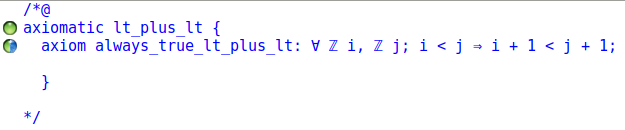
\includegraphics[scale=0.5]{5-1-1-premier-axiome.png}
\caption{Premier axiome, supposé vrai par Frama-C}
\end{figure}

\begin{zdssecretblock}{Hors sujet}
  Actuellement nos prouveurs automatiques
  n'ont pas la puissance nécessaire pour calculer \emph{la
    réponse à la grande question sur la vie, l'univers et le 
    reste}. Qu'à cela ne tienne nous pouvons le statuer comme axiome ! Reste
  à comprendre la question pour savoir où ce résultat peut-être
  utile \ldots{}
  \begin{footnotesize}\begin{Shaded}
\begin{Highlighting}[]
\CommentTokAlt{/*@}
\CommentTokAlt{  axiomatic Ax_answer_to_the_ultimate_question_of_life_the_universe_and_everything \{}
\CommentTokAlt{    logic integer the_ultimate_question_of_life_the_universe_and_everything\{L\} ;}
\CommentTokAlt{}
\CommentTokAlt{    axiom answer\{L\}:}
\CommentTokAlt{      the_ultimate_question_of_life_the_universe_and_everything\{L\} = 42;}
\CommentTokAlt{}
\CommentTokAlt{*/}
\end{Highlighting}
    \end{Shaded}
  \end{footnotesize}
\end{zdssecretblock}
  
\subsubsection{Lien avec la notion de
lemme}\label{lien-avec-la-notion-de-lemme}

Les lemmes et les axiomes vont nous permettre d'exprimer les mêmes types
de propriétés, à savoir des propriétés exprimées sur des variables
quantifiées (et éventuellement des variables globales, mais cela reste
assez rare puisqu'il est difficile de trouver une propriété qui soit
globalement vraie à leur sujet tout en étant intéressante). Outre ce
point commun, il faut également savoir que comme les axiomes, en dehors
de leur définition, les lemmes sont considérés vrais par WP.

La seule différence entre lemme et axiome du point de vue de la preuve
est donc que nous devrons fournir une preuve que le premier est valide
alors que l'axiome est toujours supposé vrai.

\subsection{Définition de fonctions ou prédicats
récursifs}\label{duxe9finition-de-fonctions-ou-pruxe9dicats-ruxe9cursifs}

Les définitions axiomatiques de fonctions ou de prédicats récursifs sont
particulièrement utiles car elles vont permettre d'empêcher les
prouveurs de dérouler la récursion quand c'est possible, notamment parce
que justement, à la manière dont nous avions ajouté un lemme sur la
factorielle nous allons pouvoir directement exprimer l'induction dans
l'axiomatique.

L'idée est alors de ne pas définir directement la fonction ou le
prédicat mais plutôt de la déclarer puis de définir des axiomes
spécifiant sont comportement. Si nous reprenons par exemple la
factorielle, nous pouvons la définir axiomatiquement de cette manière :

\begin{footnotesize}\begin{Shaded}
\begin{Highlighting}[]
\CommentTok{/*@}
\CommentTok{  axiomatic Factorial\{}
\CommentTok{    logic integer factorial(integer n);}
\CommentTok{    }
\CommentTok{    axiom factorial_0:}
\CommentTok{      \textbackslash{}forall integer i; i <= 0 ==> 1 == factorial(i) ;}

\CommentTok{    axiom factorial_n:}
\CommentTok{      \textbackslash{}forall integer i; i > 0 ==> i * factorial(i-1) == factorial(i) ;}
\CommentTok{  \}}
\CommentTok{*/}
\end{Highlighting}
\end{Shaded}\end{footnotesize}

Dans cette définition axiomatique, notre fonction n'a pas de corps. Son
comportement étant défini par les axiomes ensuite définis. Une petite
subtilité est qu'il faut prendre garde au fait que si les axiomes
statuent des propriétés à propos du contenu d'une ou plusieurs zones
mémoires pointées, il faut spécifier ces zones mémoires en utilisant la
notation \texttt{reads} au niveau de la déclaration. Si nous oublions
une telle spécification, le prédicat, ou la fonction, sera considéré
comme énoncé à propos du pointeur et non à propos de la zone mémoire
pointée. Une modification de celle-ci n'entraînera donc pas
l'invalidation d'une propriété connue axiomatiquement.

Si par exemple, nous voulons définir qu'un tableau ne contient que des
0, nous pouvons le faire de cette façon :

\begin{footnotesize}\begin{Shaded}
\begin{Highlighting}[]
\CommentTok{/*@}
\CommentTok{  axiomatic A_all_zeros\{}
\CommentTok{    predicate zeroed\{L\}(int* a, integer b, integer e) reads a[b .. e-1];}

\CommentTok{    axiom zeroed_empty\{L\}:}
\CommentTok{      \textbackslash{}forall int* a, integer b, e; b >= e ==> zeroed\{L\}(a,b,e);}

\CommentTok{    axiom zeroed_range\{L\}:}
\CommentTok{      \textbackslash{}forall int* a, integer b, e; b < e+1 ==>}
\CommentTok{        zeroed\{L\}(a,b,e+1) <==> (zeroed\{L\}(a,b,e) && a[e] == 0);}
\CommentTok{  \}}
\CommentTok{*/}
\end{Highlighting}
\end{Shaded}\end{footnotesize}

Et nous pouvons à nouveau prouver notre fonction de remise à zéro avec
cette nouvelle définition :

\begin{footnotesize}\begin{Shaded}
\begin{Highlighting}[]
\CommentTok{#include <stddef.h>}

\CommentTok{/*@}
\CommentTok{  requires \textbackslash{}valid(array + (0 .. length-1));}
\CommentTok{  assigns  array[0 .. length-1];}
\CommentTok{  ensures  zeroed(array,0,length);}
\CommentTok{*/}
\DataTypeTok{void} \NormalTok{raz(}\DataTypeTok{int}\NormalTok{* array, size_t length)\{}
  \CommentTok{/*@}
\CommentTok{    loop invariant 0 <= i <= length;}
\CommentTok{    loop invariant zeroed(array,0,i);}
\CommentTok{    loop assigns i, array[0 .. length-1];}
\CommentTok{    loop variant length-i;}
\CommentTok{  */}
  \KeywordTok{for}\NormalTok{(size_t i = }\DecValTok{0}\NormalTok{; i < length; ++i)}
    \NormalTok{array[i] = }\DecValTok{0}\NormalTok{;}
\NormalTok{\}}
\end{Highlighting}
\end{Shaded}\end{footnotesize}

Selon votre version de Frama-C et de vos prouveurs automatiques, la
preuve de préservation de l'invariant peut échouer. Une raison à cela
est que le prouveur ne parvient pas à garder l'information que ce qui
précède la cellule en cours de traitement par la boucle est toujours à
0. Nous pouvons ajouter un lemme dans notre base de connaissance,
expliquant que si l'ensemble des valeurs d'un tableau n'a pas changé,
alors la propriété est toujours vérifiée :

\begin{footnotesize}\begin{Shaded}
\begin{Highlighting}[]
\CommentTok{/*@}
\CommentTok{  predicate same_elems\{L1,L2\}(int* a, integer b, integer e) =}
\CommentTok{    \textbackslash{}forall integer i; b <= i < e ==> \textbackslash{}at(a[i],L1) == \textbackslash{}at(a[i],L2);}

\CommentTok{  lemma no_changes\{L1,L2\}:}
\CommentTok{  \textbackslash{}forall int* a, integer b, e;}
\CommentTok{  same_elems\{L1,L2\}(a,b,e) ==> zeroed\{L1\}(a,b,e) ==> zeroed\{L2\}(a,b,e);}
\CommentTok{*/}
\end{Highlighting}
\end{Shaded}\end{footnotesize}

Et d'énoncer une assertion pour spécifier ce qui n'a pas changé entre le
début du bloc de la boucle (marqué par le label \texttt{L} dans le code)
et la fin (qui se trouve être \texttt{Here} puisque nous posons notre
assertion à la fin) :

\begin{footnotesize}\begin{Shaded}
\begin{Highlighting}[]
\KeywordTok{for}\NormalTok{(size_t i = }\DecValTok{0}\NormalTok{; i < length; ++i)\{}
  \NormalTok{L:}
  \NormalTok{array[i] = }\DecValTok{0}\NormalTok{;}
  \CommentTok{//@ assert same_elems\{L,Here\}(array,0,i);}
\NormalTok{\}}
\end{Highlighting}
\end{Shaded}\end{footnotesize}

À noter que dans cette nouvelle version du code, la propriété énoncée
par notre lemme n'est pas prouvée par les solveurs automatiques, qui ne
savent pas raisonner pas induction. Pour les curieux, la (très simple)
preuve en Coq est ci-dessous :

\begin{zdssecretblock}{Preuve Coq}
  \begin{footnotesize}
  \begin{footnotesize}\begin{Shaded}
\begin{Highlighting}[]
(* Généré par WP *)
Definition P_same_elems (Mint_0 : farray addr Z) (Mint_1 : farray addr Z)
    (a : addr) (b : Z) (e : Z) : Prop :=
    forall (i : Z), let a_1 := (shift_sint32 a i%Z) in ((b <= i)%Z) ->
      ((i < e)%Z) -> (((Mint_0.[ a_1 ]) = (Mint_1.[ a_1 ]))%Z).
Goal
  forall (i_1 i : Z), forall (t_1 t : farray addr Z), forall (a : addr),
  ((P_zeroed t a i_1%Z i%Z)) ->
    ((P_same_elems t_1 t a i_1%Z i%Z)) ->
      ((P_zeroed t_1 a i_1%Z i%Z)).
(* Notre preuve *)
Proof.
  intros b e.
  (* par induction sur la distance entre b et e *)
  induction e using Z_induction with (m := b) ; intros mem_l2 mem_l1 a Hz_l1 Hsame.
  (* cas de base : Axiome "empty" *)
  + apply A_A_all_zeros.Q_zeroed_empty ; assumption.
  + replace (e + 1) with (1 + e) in * ; try omega.
    (* on utilise l'axiome range *)
    rewrite A_A_all_zeros.Q_zeroed_range in * ; intros Hinf.
    apply Hz_l1 in Hinf ; clear Hz_l1 ; inversion_clear Hinf as [Hlast Hothers].
    split.
    (* sous plage de Hsame *)
    - rewrite Hsame ; try assumption ; omega.
    (* hypothèse d'induction *)
    - apply IHe with (t := mem_l1) ; try assumption.
      * unfold P_same_elems ; intros ; apply Hsame ; omega.
Qed.
\end{Highlighting}
  \end{Shaded}\end{footnotesize}
  \end{footnotesize}
\end{zdssecretblock}

Dans le cas présent, utiliser une axiomatique est contre-productif :
notre propriété est très facilement exprimable en logique du premier
ordre comme nous l'avons déjà fait précédemment. Les axiomatiques sont
faites pour écrire des définitions qui ne sont pas simples à exprimer
dans le formalisme de base d'ACSL. Mais il est mieux de commencer avec
un exemple facile à lire.

\subsection{Consistance}\label{consistance}

En ajoutant des axiomes à notre base de connaissances, nous pouvons
produire des preuves plus complexes car certaines parties de cette
preuve, mentionnées par les axiomes, ne nécessiteront plus de preuves
qui allongeraient le processus complet. Seulement, en faisant cela
\textbf{nous devons être extrêmement prudents}. En effet, la moindre
hypothèse fausse introduite dans la base pourraient rendre tous nos
raisonnements futiles. Notre raisonnement serait toujours correct, mais
basé sur des connaissances fausses, il nous apprendrait plus rien de
correct.

L'exemple le plus simple à produire est le suivant:

\begin{footnotesize}\begin{Shaded}
\begin{Highlighting}[]
\CommentTok{/*@}
\CommentTok{  axiomatic False\{}
\CommentTok{    axiom false_is_true: \textbackslash{}false;}
\CommentTok{  \}}
\CommentTok{*/}

\DataTypeTok{int} \NormalTok{main()\{}
  \CommentTok{// Exemples de propriétés prouvées}

  \CommentTok{//@ assert \textbackslash{}false;}
  \CommentTok{//@ assert \textbackslash{}forall integer x; x > x;}
  \CommentTok{//@ assert \textbackslash{}forall integer x,y,z ; x == y == z == 42;}
  \KeywordTok{return} \NormalTok{*(}\DataTypeTok{int}\NormalTok{*) }\DecValTok{0}\NormalTok{;}
\NormalTok{\}}
\end{Highlighting}
\end{Shaded}\end{footnotesize}

Et tout est prouvé, y compris que le déréférencement de l'adresse 0 est
OK :

\begin{figure}[htbp]
\centering
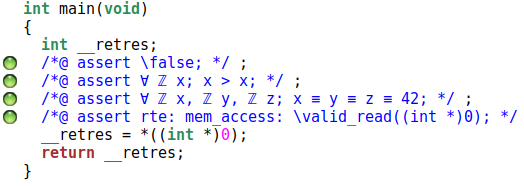
\includegraphics[scale=0.5]{false_axiom.png}
\caption{Preuve de tout un tas de choses fausses}
\end{figure}

Évidemment cet exemple est extrême, nous n'écririons pas un tel axiome.
Le problème est qu'il est très facile d'écrire une axiomatique
subtilement fausse lorsque nous exprimons des propriétés plus complexe,
ou que nous commençons à poser des suppositions sur l'état global d'un
système.

Quand nous commençons à faire créer de telles définitions, ajouter de
temps en temps une preuve ponctuelle de \og{}false\fg{} dont nous voulons
qu'elle échoue permet de s'assurer que notre définition n'est pas
inconsistante. Mais cela ne fait pas tout ! Si la subtilité qui crée le
comportement faux est suffisamment cachée, les prouveurs peuvent avoir
besoin de beaucoup d'informations autre que l'axiomatique elle-même pour
être menés jusqu'à l'inconsistance, donc il faut toujours être vigilant
!

Notamment parce que par exemple, la mention des valeurs lues par une
fonction ou un prédicat défini axiomatiquement est également importante
pour la consistance de l'axiomatique. En effet, comme mentionné
précédemment, si nous n'exprimons pas les valeurs lues dans le cas de
l'usage d'un pointeur, la modification d'une valeur du tableau
n'invalide pas une propriété de ce type d'un tableau par exemple. Dans
un tel cas, la preuve passe mais l'axiome n'exprimant pas le contenu,
nous ne prouvons rien.

Par exemple, si nous reprenons l'exemple de mise à zéro, nous pouvons
modifier la définition de notre axiomatique en retirant la mention des
valeurs dont dépendent le prédicat : \texttt{reads\ a{[}b\ ..\ e-1{]}}.
La preuve passera toujours mais n'exprimera plus rien à propos du
contenu des tableaux considérés.

\subsection{Exemple : comptage de
valeurs}\label{exemple-comptage-de-valeurs}

Dans cet exemple, nous cherchons à prouver qu'un algorithme compte bien
les occurrences d'une valeur dans un tableau. Nous commençons par
définir axiomatiquement la notion de comptage dans un tableau :

\begin{footnotesize}\begin{Shaded}
\begin{Highlighting}[]
\CommentTok{/*@}
\CommentTok{  axiomatic Occurrences_Axiomatic\{}
\CommentTok{    logic integer l_occurrences_of\{L\}(int value, int* in, integer from, integer to)}
\CommentTok{      reads in[from .. to-1];}

\CommentTok{    axiom occurrences_empty_range\{L\}:}
\CommentTok{      \textbackslash{}forall int v, int* in, integer from, to;}
\CommentTok{        from >= to ==> l_occurrences_of\{L\}(v, in, from, to) == 0;}
\CommentTok{    }
\CommentTok{    axiom occurrences_positive_range_with_element\{L\}:}
\CommentTok{      \textbackslash{}forall int v, int* in, integer from, to;}
\CommentTok{        (from < to+1 && in[to] == v) ==>}
\CommentTok{      l_occurrences_of(v,in,from,to+1) == 1+l_occurrences_of(v,in,from,to);}

\CommentTok{    axiom occurrences_positive_range_without_element\{L\}:}
\CommentTok{      \textbackslash{}forall int v, int* in, integer from, to;}
\CommentTok{        (from < to+1 && in[to] != v) ==>}
\CommentTok{      l_occurrences_of(v,in,from,to+1) == l_occurrences_of(v,in,from,to);}
\CommentTok{  \}}
\CommentTok{*/}
\end{Highlighting}
\end{Shaded}\end{footnotesize}

Nous avons trois cas à gérer :

\begin{itemize}
\tightlist
\item
  la plage de valeur concernée est vide : le nombre d'occurrences est 0
  ;
\item
  la plage de valeur n'est pas vide et le dernier élément est celui
  recherché : le nombre d'occurrences est le nombre d'occurrences dans
  la plage privée du dernier élément plus 1 ;
\item
  la plage de valeur n'est pas vide et le dernier élément n'est pas
  celui recherché : le nombre d'occurrences est le nombre d'occurrences
  dans la plage privée du dernier élément.
\end{itemize}

Par la suite, nous pouvons écrire la fonction C exprimant ce
comportement et la prouver :

\begin{footnotesize}\begin{Shaded}
\begin{Highlighting}[]
\CommentTok{/*@}
\CommentTok{  requires \textbackslash{}valid_read(in+(0 .. length));}
\CommentTok{  assigns  \textbackslash{}nothing;}
\CommentTok{  ensures  \textbackslash{}result == l_occurrences_of(value, in, 0, length);}
\CommentTok{*/}
\NormalTok{size_t occurrences_of(}\DataTypeTok{int} \NormalTok{value, }\DataTypeTok{int}\NormalTok{* in, size_t length)\{}
  \NormalTok{size_t result = }\DecValTok{0}\NormalTok{;}
  
  \CommentTok{/*@}
\CommentTok{    loop invariant 0 <= result <= i <= length;}
\CommentTok{    loop invariant result == l_occurrences_of(value, in, 0, i);}
\CommentTok{    loop assigns i, result;}
\CommentTok{    loop variant length-i;}
\CommentTok{  */}
  \KeywordTok{for}\NormalTok{(size_t i = }\DecValTok{0}\NormalTok{; i < length; ++i)}
    \NormalTok{result += (in[i] == value)? }\DecValTok{1} \NormalTok{: }\DecValTok{0}\NormalTok{;}

  \KeywordTok{return} \NormalTok{result;}
\NormalTok{\}}
\end{Highlighting}
\end{Shaded}\end{footnotesize}

Une alternative au fait de spécifier que dans ce code \texttt{result}
est au maximum \texttt{i} est d'exprimer un lemme plus général à propos
de la valeur du nombre d'occurrences, dont nous ne savons qu'elle est
comprise entre 0 et la taille maximale de la plage de valeurs considérée
:

\begin{footnotesize}\begin{Shaded}
\begin{Highlighting}[]
\CommentTok{/*@}
\CommentTok{lemma l_occurrences_of_range\{L\}:}
\CommentTok{  \textbackslash{}forall int v, int* array, integer from, to:}
\CommentTok{    from <= to ==> 0 <= l_occurrences_of(v, a, from, to) <= to-from;}
\CommentTok{*/}
\end{Highlighting}
\end{Shaded}\end{footnotesize}

La preuve de ce lemme ne pourra pas être déchargée par un solveur
automatique. Il faudra faire cette preuve interactivement avec Coq par
exemple. Exprimer des lemmes généraux prouvés manuellement est souvent
une bonne manière d'ajouter des outils aux prouveurs pour manipuler plus
efficacement les axiomatiques, sans ajouter formellement d'axiomes qui
augmenteraient nos chances d'introduire des erreurs. Ici, nous devrons
quand même réaliser les preuves des propriétés mentionnées.

\subsection{Exemple : le tri}\label{exemple-le-tri}

Nous allons prouver un simple tri par sélection :

\begin{footnotesize}\begin{Shaded}
\begin{Highlighting}[]
\NormalTok{size_t min_idx_in(}\DataTypeTok{int}\NormalTok{* a, size_t beg, size_t end)\{}
  \NormalTok{size_t min_i = beg;}
  \KeywordTok{for}\NormalTok{(size_t i = beg}\DecValTok{+1}\NormalTok{; i < end; ++i)}
    \KeywordTok{if}\NormalTok{(a[i] < a[min_i]) min_i = i;}
  \KeywordTok{return} \NormalTok{min_i;}
\NormalTok{\}}

\DataTypeTok{void} \NormalTok{swap(}\DataTypeTok{int}\NormalTok{* p, }\DataTypeTok{int}\NormalTok{* q)\{}
  \DataTypeTok{int} \NormalTok{tmp = *p; *p = *q; *q = tmp;}
\NormalTok{\}}

\DataTypeTok{void} \NormalTok{sort(}\DataTypeTok{int}\NormalTok{* a, size_t beg, size_t end)\{}
  \KeywordTok{for}\NormalTok{(size_t i = beg ; i < end ; ++i)\{}
    \NormalTok{size_t imin = min_idx_in(a, i, end);}
    \NormalTok{swap(&a[i], &a[imin]);}
  \NormalTok{\}}
\NormalTok{\}}
\end{Highlighting}
\end{Shaded}\end{footnotesize}

Le lecteur pourra s'exercer en spécifiant et en prouvant les fonctions
de recherche de minimum et d'échange de valeur. Nous cachons la
correction ci-dessous et allons nous concentrer plutôt sur la
spécification et la preuve de la fonction de tri qui sont une
illustration intéressant de l'usage des axiomatiques.

\begin{zdssecretblock}{Solution}
  \begin{footnotesize}
  \begin{footnotesize}\begin{Shaded}
\begin{Highlighting}[]
\CommentTok{/*@}
\CommentTok{  requires \textbackslash{}valid_read(a + (beg .. end-1));}
\CommentTok{  requires beg < end;}

\CommentTok{  assigns  \textbackslash{}nothing;}

\CommentTok{  ensures  \textbackslash{}forall integer i; beg <= i < end ==> a[\textbackslash{}result] <= a[i];}
\CommentTok{  ensures  beg <= \textbackslash{}result < end;}
\CommentTok{*/}
\NormalTok{size_t min_idx_in(}\DataTypeTok{int}\NormalTok{* a, size_t beg, size_t end)\{}
  \NormalTok{size_t min_i = beg;}

  \CommentTok{/*@}
\CommentTok{    loop invariant beg <= min_i < i <= end;}
\CommentTok{    loop invariant \textbackslash{}forall integer j; beg <= j < i ==> a[min_i] <= a[j];}
\CommentTok{    loop assigns min_i, i;}
\CommentTok{    loop variant end-i;}
\CommentTok{  */}
  \KeywordTok{for}\NormalTok{(size_t i = beg}\DecValTok{+1}\NormalTok{; i < end; ++i)\{}
    \KeywordTok{if}\NormalTok{(a[i] < a[min_i]) min_i = i;}
  \NormalTok{\}}
  \KeywordTok{return} \NormalTok{min_i;}
\NormalTok{\}}

\CommentTok{/*@}
\CommentTok{  requires \textbackslash{}valid(p) && \textbackslash{}valid(q);}
\CommentTok{  assigns  *p, *q;}
\CommentTok{  ensures  *p == \textbackslash{}old(*q) && *q == \textbackslash{}old(*p);}
\CommentTok{*/}
\DataTypeTok{void} \NormalTok{swap(}\DataTypeTok{int}\NormalTok{* p, }\DataTypeTok{int}\NormalTok{* q)\{}
  \DataTypeTok{int} \NormalTok{tmp = *p; *p = *q; *q = tmp;}
\NormalTok{\}}
\end{Highlighting}
  \end{Shaded}\end{footnotesize}
  \end{footnotesize}
\end{zdssecretblock}
  
En effet, une erreur commune que nous pourrions faire dans le cas de la
preuve du tri est de poser cette spécification (qui est vraie !) :

\begin{footnotesize}\begin{Shaded}
\begin{Highlighting}[]
\CommentTok{/*@}
\CommentTok{  predicate sorted(int* a, integer b, integer e) =}
\CommentTok{    \textbackslash{}forall integer i, j; b <= i <= j < e ==> a[i] <= a[j];}
\CommentTok{*/}

\CommentTok{/*@}
\CommentTok{  requires \textbackslash{}valid(a + (beg .. end-1));}
\CommentTok{  requires beg < end;}
\CommentTok{  assigns  a[beg .. end-1];}
\CommentTok{  ensures sorted(a, beg, end);}
\CommentTok{*/}
\DataTypeTok{void} \NormalTok{sort(}\DataTypeTok{int}\NormalTok{* a, size_t beg, size_t end)\{}
  \CommentTok{/*@ //annotation de l'invariant */}
  \KeywordTok{for}\NormalTok{(size_t i = beg ; i < end ; ++i)\{}
    \NormalTok{size_t imin = min_idx_in(a, i, end);}
    \NormalTok{swap(&a[i], &a[imin]);}
  \NormalTok{\}}
\NormalTok{\}}
\end{Highlighting}
\end{Shaded}\end{footnotesize}

\textbf{Cette spécification est vraie}. Mais si nous nous rappelons la
partie concernant les spécifications, nous nous devons d'exprimer
précisément ce que nous attendons. Avec la spécification actuelle, nous
ne prouvons pas toutes les propriétés nécessaires d'un tri ! Par
exemple, cette fonction remplit pleinement la spécification :

\begin{footnotesize}\begin{Shaded}
\begin{Highlighting}[]
\CommentTok{/*@}
\CommentTok{  requires \textbackslash{}valid(a + (beg .. end-1));}
\CommentTok{  requires beg < end;}

\CommentTok{  assigns  a[beg .. end-1];}
\CommentTok{  }
\CommentTok{  ensures sorted(a, beg, end);}
\CommentTok{*/}
\DataTypeTok{void} \NormalTok{fail_sort(}\DataTypeTok{int}\NormalTok{* a, size_t beg, size_t end)\{}
  \CommentTok{/*@}
\CommentTok{    loop invariant beg <= i <= end;}
\CommentTok{    loop invariant \textbackslash{}forall integer j; beg <= j < i ==> a[j] == 0;}
\CommentTok{    loop assigns i, a[beg .. end-1];}
\CommentTok{    loop variant end-i;}
\CommentTok{  */}
  \KeywordTok{for}\NormalTok{(size_t i = beg ; i < end ; ++i)}
    \NormalTok{a[i] = }\DecValTok{0}\NormalTok{;}
\NormalTok{\}}
\end{Highlighting}
\end{Shaded}\end{footnotesize}

En fait notre spécification oublie que tous les éléments qui étaient
originellement présents dans le tableau à l'appel de la fonction doivent
toujours être présents après l'exécution de notre fonction de tri. Dit
autrement, notre fonction doit en fait produire la permutation triée des
valeurs du tableau.

Une propriété comme la définition de ce qu'est une permutation s'exprime
extrêmement bien par l'utilisation d'une axiomatique. En effet, pour
déterminer qu'un tableau est la permutation d'un autre, les cas sont
très limités. Premièrement, le tableau est une permutation de lui-même,
puis l'échange de deux valeurs sans changer les autres est également une
permutation, et finalement si nous créons la permutation \(p_2\) d'une
permutation \(p_1\), puis que nous créons la permutation \(p_3\) de
\(p_2\), alors par transitivité \(p_3\) est une permutation de \(p_1\).

Ceci est exprimé par le code suivant :

\begin{footnotesize}\begin{Shaded}
\begin{Highlighting}[]
\CommentTok{/*@}
\CommentTok{  predicate swap_in_array\{L1,L2\}(int* a, integer b, integer e, integer i, integer j) =}
\CommentTok{    b <= i < e && b <= j < e &&}
\CommentTok{    \textbackslash{}at(a[i], L1) == \textbackslash{}at(a[j], L2) && \textbackslash{}at(a[j], L1) == \textbackslash{}at(a[i], L2) &&}
\CommentTok{    \textbackslash{}forall integer k; b <= k < e && k != j && k != i ==> \textbackslash{}at(a[k], L1) == \textbackslash{}at(a[k], L2);}

\CommentTok{  axiomatic Permutation\{}
\CommentTok{    predicate permutation\{L1,L2\}(int* a, integer b, integer e)}
\CommentTok{     reads \textbackslash{}at(*(a+(b .. e - 1)), L1), \textbackslash{}at(*(a+(b .. e - 1)), L2);}

\CommentTok{    axiom reflexive\{L1\}: }
\CommentTok{      \textbackslash{}forall int* a, integer b,e ; permutation\{L1,L1\}(a, b, e);}

\CommentTok{    axiom swap\{L1,L2\}:}
\CommentTok{      \textbackslash{}forall int* a, integer b,e,i,j ;}
\CommentTok{        swap_in_array\{L1,L2\}(a,b,e,i,j) ==> permutation\{L1,L2\}(a, b, e);}
\CommentTok{    }
\CommentTok{    axiom transitive\{L1,L2,L3\}:}
\CommentTok{      \textbackslash{}forall int* a, integer b,e ; }
\CommentTok{        permutation\{L1,L2\}(a, b, e) && permutation\{L2,L3\}(a, b, e) ==>}
\CommentTok{          permutation\{L1,L3\}(a, b, e);}
\CommentTok{  \}}
\CommentTok{*/}
\end{Highlighting}
\end{Shaded}\end{footnotesize}

Nous spécifions alors que notre tri nous crée la permutation triée du
tableau d'origine et nous pouvons prouver l'ensemble en complétant
l'invariant de la fonction :

\begin{footnotesize}\begin{Shaded}
\begin{Highlighting}[]
\CommentTok{/*@}
\CommentTok{  requires beg < end && \textbackslash{}valid(a + (beg .. end-1));}
\CommentTok{  assigns  a[beg .. end-1];  }
\CommentTok{  ensures sorted(a, beg, end);}
\CommentTok{  ensures permutation\{Pre, Post\}(a,beg,end);}
\CommentTok{*/}
\DataTypeTok{void} \NormalTok{sort(}\DataTypeTok{int}\NormalTok{* a, size_t beg, size_t end)\{}
  \CommentTok{/*@}
\CommentTok{    loop invariant beg <= i <= end;}
\CommentTok{    loop invariant sorted(a, beg, i) && permutation\{Begin, Here\}(a, beg, end);}
\CommentTok{    loop invariant \textbackslash{}forall integer j,k; beg <= j < i ==> i <= k < end ==> a[j] <= a[k];}
\CommentTok{    loop assigns i, a[beg .. end-1];}
\CommentTok{    loop variant end-i;}
\CommentTok{  */}
  \KeywordTok{for}\NormalTok{(size_t i = beg ; i < end ; ++i)\{}
    \CommentTok{//@ ghost begin: ;}
    \NormalTok{size_t imin = min_idx_in(a, i, end);}
    \NormalTok{swap(&a[i], &a[imin]);}
    \CommentTok{//@ assert swap_in_array\{begin,Here\}(a,beg,end,i,imin);}
  \NormalTok{\}}
\NormalTok{\}}
\end{Highlighting}
\end{Shaded}\end{footnotesize}

Cette fois, notre propriété est précisément définie, la preuve reste
assez simple à faire passer, ne nécessitant que l'ajout d'une assertion
que le bloc de la fonction n'effectue qu'un échange des valeurs dans le
tableau (et donnant ainsi la transition vers la permutation suivante du
tableau. Pour définir cette notion d'échange, nous utilisons une
annotation particulière (à la ligne 16), introduite par le mot-clé
\texttt{ghost}. Ici, le but est d'introduire un label fictif dans le
code qui est uniquement visible d'un point de vue spécification. C'est
l'objet de la prochaine section.

\section{Code Fantôme}\label{code-fantuxf4me}

Derrière ce titre faisant penser à un scénario de film d'action se cache
en fait un moyen d'enrichir la spécification avec des informations sous
la forme de code en langage C. Ici, l'idée va être d'ajouter des
variables et du code source qui n'interviendra pas dans le programme
réel mais permettant de créer des états logiques qui ne seront visibles
que depuis la preuve. Par cet intermédiaire, nous pouvons rendre
explicites des propriétés logiques qui étaient auparavant implicites.

\subsection{Syntaxe}\label{syntaxe-4}

Le code fantôme est ajouté par l'intermédiaire d'annotations qui vont
contenir du code C ainsi que la mention \texttt{ghost}.

\begin{footnotesize}\begin{Shaded}
\begin{Highlighting}[]
\CommentTok{/*@}
\CommentTok{  ghost}
\CommentTok{  // code en langage C}
\CommentTok{*/}
\end{Highlighting}
\end{Shaded}\end{footnotesize}

Les seules règles que nous devons respecter dans un tel code est que
nous ne devons jamais écrire une portion de mémoire qui n'est pas
elle-même définie dans du code fantôme et que le code en question doit
terminer tout bloc qu'il ouvrirait. Mis à par cela, tout calcul peut
être inséré tant qu'il n'écrit pas la mémoire.

Voici quelques exemples pour la syntaxe de code fantôme :

\begin{footnotesize}\begin{Shaded}
\begin{Highlighting}[]
\CommentTok{//@ ghost int ghost_glob_var = 0;}

\DataTypeTok{void} \NormalTok{foo(}\DataTypeTok{int} \NormalTok{a)\{}
  \CommentTok{//@ ghost int ghost_loc_var = a;}

  \CommentTok{//@ ghost Ghost_label: ;}
  \NormalTok{a = }\DecValTok{28} \NormalTok{;}

  \CommentTok{//@ ghost if(a < 0)\{ ghost_loc_var = 0; \}}

  \CommentTok{//@ assert ghost_loc_var == \textbackslash{}at(a, Ghost_label) == \textbackslash{}at(a, Pre);}
\NormalTok{\}}
\end{Highlighting}
\end{Shaded}\end{footnotesize}

Il faut être très prudent lorsque nous produisons ce genre de code. En
effet, aucune vérification n'est effectuée pour s'assurer que nous
n'écrivons pas dans la mémoire globale par erreur. Ce problème étant
comme la vérification elle-même, un problème indécidable, une telle
analyse serait un travail de preuve à part entière. Par exemple, ce code
est accepté en entrée de Frama-C, alors qu'il modifie manifestement
l'état de la mémoire du programme :

\begin{footnotesize}\begin{Shaded}
\begin{Highlighting}[]
\DataTypeTok{int} \NormalTok{a;}

\DataTypeTok{void} \NormalTok{foo()\{}
  \CommentTok{//@ ghost a = 42;}
\NormalTok{\}}
\end{Highlighting}
\end{Shaded}\end{footnotesize}

Il faut donc faire très attention à ce que nous faisons avec du code
fantôme.

\subsection{Expliciter un état
logique}\label{expliciter-un-uxe9tat-logique}

Le but du code ghost est de rendre explicite des informations
généralement implicites. Par exemple, dans la section précédente, nous
nous en sommes servi pour récupérer explicitement un état logique connu
à un point de programme donné.

Prenons maintenant un exemple plus poussé. Nous voulons par exemple
prouver que la fonction suivante nous retourne la valeur maximale des
sommes de sous tableaux possibles d'un tableau donné. Un sous-tableau
d'un tableau \og{}a\fg{} est un sous-ensemble contigu de valeur de \og{}a\fg{}. Par
exemple, pour un tableau \texttt{\{\ 0\ ,\ 3\ ,\ -1\ ,\ 4\ \}}, des
exemples de sous tableaux peuvent être \texttt{\{\}},
\texttt{\{\ 0\ \}}, \texttt{\{\ 3\ ,\ -1\ \}} ,
\texttt{\{\ 0\ ,\ 3\ ,\ -1\ ,\ 4\ \}}, \ldots{} Notez que comme nous
autorisons le tableau vide, la somme est toujours au moins égale à 0.
Dans le tableau précédent, le sous tableau de valeur maximale est
\texttt{\{\ 3\ ,\ -1\ ,\ 4\ \}}, la fonction renverra donc 6.

\begin{footnotesize}\begin{Shaded}
\begin{Highlighting}[]
\DataTypeTok{int} \NormalTok{max_subarray(}\DataTypeTok{int} \NormalTok{*a, size_t len) \{}
  \DataTypeTok{int} \NormalTok{max = }\DecValTok{0}\NormalTok{;}
  \DataTypeTok{int} \NormalTok{cur = }\DecValTok{0}\NormalTok{;}
  \KeywordTok{for}\NormalTok{(size_t i = }\DecValTok{0}\NormalTok{; i < len; i++) \{}
    \NormalTok{cur += a[i];}
    \KeywordTok{if} \NormalTok{(cur < }\DecValTok{0}\NormalTok{)   cur = }\DecValTok{0}\NormalTok{;}
    \KeywordTok{if} \NormalTok{(cur > max) max = cur;}
  \NormalTok{\}}
  \KeywordTok{return} \NormalTok{max;}
\NormalTok{\}}
\end{Highlighting}
\end{Shaded}\end{footnotesize}

Pour spécifier la fonction précédente, nous allons avoir besoin
d'exprimer axiomatiquement la somme. Ce n'est pas très complexe, et le
lecteur pourra s'exercer en exprimant les axiomes nécessaires au bon
fonctionnement de cette axiomatique :

\begin{footnotesize}\begin{Shaded}
\begin{Highlighting}[]
\CommentTok{/*@ axiomatic Sum \{}
\CommentTok{  logic integer sum(int *array, integer begin, integer end) reads a[begin..(end-1)];}
\CommentTok{\}*/}
\end{Highlighting}
\end{Shaded}\end{footnotesize}

\begin{zdssecretblock}{Solution}
\begin{footnotesize}\begin{Shaded}
\begin{Highlighting}[]
\CommentTok{/*@}
\CommentTok{  axiomatic Sum_array\{}
\CommentTok{    logic integer sum(int* array, integer begin, integer end) }
\CommentTok{      reads array[begin .. (end-1)];}
\CommentTok{   }
\CommentTok{    axiom empty: }
\CommentTok{      \textbackslash{}forall int* a, integer b, e; b >= e ==> sum(a,b,e) == 0;}
\CommentTok{    axiom range:}
\CommentTok{      \textbackslash{}forall int* a, integer b, e; b < e ==> sum(a,b,e) == sum(a,b,e-1)+a[e-1];}
\CommentTok{  \}}
\CommentTok{*/}
\end{Highlighting}
\end{Shaded}\end{footnotesize}
\end{zdssecretblock}

La spécification de notre fonction est la suivante :

\begin{footnotesize}\begin{Shaded}
\begin{Highlighting}[]
\CommentTok{/*@ }
\CommentTok{  requires \textbackslash{}valid(a+(0..len-1));}
\CommentTok{  assigns \textbackslash{}nothing;}
\CommentTok{  ensures \textbackslash{}forall integer l, h;  0 <= l <= h <= len ==> sum(a,l,h) <= \textbackslash{}result;}
\CommentTok{  ensures \textbackslash{}exists integer l, h;  0 <= l <= h <= len &&  sum(a,l,h) == \textbackslash{}result;}
\CommentTok{*/}
\end{Highlighting}
\end{Shaded}\end{footnotesize}

Pour toute paire de bornes la valeur retournée doit être supérieure ou
égale et il doit exister une paire telle que c'est égal. Par rapport à
cette spécification, si nous devons ajouter les invariants de boucles,
nous nous apercevons rapidement qu'il va nous manquer des informations.
Nous avons besoin d'exprimer ce que sont les valeurs \texttt{max} et
\texttt{cur} et quelles relations il existe entre elles, mais rien ne
nous le permet !

En substance, notre post-condition a besoin de savoir qu'il existe des
bornes \texttt{low} et \texttt{high} telles que la somme calculée
correspond à ces bornes. Or notre code, n'exprime rien de tel d'un point
de vue logique et rien ne nous permet \emph{a priori} de faire cette
liaison en utilisant des formulations logiques. Nous allons donc
utiliser du code ghost pour conserver ces bornes et exprimer l'invariant
de notre boucle.

Nous allons d'abord avoir besoin de 2 variables qui vont nous permettre
de stocker les valeurs des bornes de la plage maximum, nous les
appellerons \texttt{low} et \texttt{high}. Chaque fois que nous
trouverons une plage où la somme est plus élevée nous le mettrons à
jour. Ces bornes correspondront donc à la somme indiquée par
\texttt{max}. Cela induit que nous avons encore besoin d'une autre paire
de bornes : celle correspondant à la variable de somme \texttt{cur} à
partir de laquelle nous pourrons construire les bornes de \texttt{max}.
Pour celle-ci, nous n'avons besoin que d'ajouter une variable ghost : le
minimum actuel \texttt{cur\_low}, la borne supérieure de la somme
actuelle étant indiquée par la variable \texttt{i} de la boucle.

\begin{footnotesize}\begin{Shaded}
\begin{Highlighting}[]
\CommentTok{/*@ }
\CommentTok{  requires \textbackslash{}valid(a+(0..len-1));}
\CommentTok{  assigns \textbackslash{}nothing;}
\CommentTok{  ensures \textbackslash{}forall integer l, h;  0 <= l <= h <= len ==> sum(a,l,h) <= \textbackslash{}result;}
\CommentTok{  ensures \textbackslash{}exists integer l, h;  0 <= l <= h <= len &&  sum(a,l,h) == \textbackslash{}result;}
\CommentTok{*/}
\DataTypeTok{int} \NormalTok{max_subarray(}\DataTypeTok{int} \NormalTok{*a, size_t len) \{}
  \DataTypeTok{int} \NormalTok{max = }\DecValTok{0}\NormalTok{;}
  \DataTypeTok{int} \NormalTok{cur = }\DecValTok{0}\NormalTok{;}
  \CommentTok{//@ ghost size_t cur_low = 0; }
  \CommentTok{//@ ghost size_t low = 0;}
  \CommentTok{//@ ghost size_t high = 0; }

  \CommentTok{/*@ }
\CommentTok{    loop invariant BOUNDS: low <= high <= i <= len && cur_low <= i;}
\CommentTok{    }
\CommentTok{    loop invariant REL :   cur == sum(a,cur_low,i) <= max == sum(a,low,high);}
\CommentTok{    loop invariant POST:   \textbackslash{}forall integer l;    0 <= l <= i      ==> sum(a,l,i) <= cur;}
\CommentTok{    loop invariant POST:   \textbackslash{}forall integer l, h; 0 <= l <= h <= i ==> sum(a,l,h) <= max;}
\CommentTok{   }
\CommentTok{    loop assigns i, cur, max, cur_low, low, high;}
\CommentTok{    loop variant len - i; }
\CommentTok{  */}
  \KeywordTok{for}\NormalTok{(size_t i = }\DecValTok{0}\NormalTok{; i < len; i++) \{}
    \NormalTok{cur += a[i];}
    \KeywordTok{if} \NormalTok{(cur < }\DecValTok{0}\NormalTok{) \{}
      \NormalTok{cur = }\DecValTok{0}\NormalTok{;}
      \CommentTok{/*@ ghost cur_low = i+1; */}
    \NormalTok{\}}
    \KeywordTok{if} \NormalTok{(cur > max) \{}
      \NormalTok{max = cur;}
      \CommentTok{/*@ ghost low = cur_low; */}
      \CommentTok{/*@ ghost high = i+1; */}
    \NormalTok{\}}
  \NormalTok{\}}
  \KeywordTok{return} \NormalTok{max;}
\NormalTok{\}}
\end{Highlighting}
\end{Shaded}\end{footnotesize}

L'invariant \texttt{BOUNDS} exprime comment sont ordonnées les
différentes bornes pendant le calcul. L'invariant \texttt{REL} exprime
ce que signifient les valeurs \texttt{cur} et \texttt{max} par rapport à
ces bornes. Finalement, l'invariant \texttt{POST} permet de faire le
lien entre les invariants précédents et la post-condition de la
fonction.

Le lecteur pourra vérifier que cette fonction est effectivement prouvée
sans la vérification des RTE. Si nous ajoutons également le contrôle des
RTE, nous pouvons voir que le calcul de la somme indique un dépassement
possible sur les entiers.

Ici, nous ne chercherons pas à le corriger car ce n'est pas l'objet de
l'exemple. Le moyen de prouver cela dépend en fait fortement du contexte
dans lequel on utilise la fonction. Une possibilité est de restreindre
fortement le contrat en imposant des propriétés à propos des valeurs et
de la taille du tableau. Par exemple : nous pourrions imposer une taille
maximale et des bornes fortes pour chacune des cellules. Une autre
possibilité est d'ajouter une valeur d'erreur en cas de dépassement (par
exemple \(-1\)), et de spécifier qu'en cas de dépassement, c'est cette
valeur qui est renvoyée.

Dans cette partie, nous avons vu des constructions plus avancées du
langage ACSL qui nous permettent d'exprimer et de prouver des propriétés
plus complexes à propos de nos programmes.

Mal utilisées, ces fonctionnalités peuvent fausser nos analyses, il faut
donc se montrer attentif lorsque nous manipulons ces constructions et ne
pas hésiter à les relire ou encore à exprimer des propriétés à vérifier
à leur sujet afin de s'assurer que nous ne sommes pas en train
d'introduire des incohérences dans notre programme ou nos hypothèses de
travail.

\chapter{Conclusion}\label{conclusion}

\begin{quote}
  Voilà, c'est fini \ldots{}

  Jean-Louis Aubert, \emph{Bleu Blanc Vert}, 1989
\end{quote}

\ldots{} pour cette introduction à la preuve de programmes avec Frama-C
et WP.

Tout au long de ce tutoriel, nous avons pu voir comment utiliser ces
outils pour spécifier ce que nous attendons de nos programmes et
vérifier que le code que nous avons produit correspond effectivement à
la spécification que nous en avons faite. Cette spécification passe par
l'annotation de nos fonctions avec le contrat qu'elle doit respecter,
c'est-à-dire les propriétés que doivent respecter les entrées de la
fonction pour garantir son bon fonctionnement et les propriétés que
celle-ci s'engage à assurer sur les sorties en retour.

À partir de nos programmes spécifiés, WP est capable de produire un
raisonnement nous disant si oui, ou non, notre programme répond au
besoin exprimé. La forme de raisonnement utilisée étant complètement
modulaire, elle nous permet de prouver les fonctions une à une et de les
composer. WP ne comprend pas, à l'heure actuelle, l'allocation
dynamique. Une fonction qui en utiliserait ne pourrait donc pas être
prouvée.

Mais même sans cela, une large variété de fonctions n'ont pas besoin
d'effectuer d'allocation dynamique, travaillant donc sur des données
déjà allouées. Et ces fonctions peuvent ensuite être appelées avec
l'assurance qu'elles font correctement leur travail. Si nous ne voulons
pas prouver le code appelant, nous pouvons toujours écrire quelque chose
comme cela :

\begin{footnotesize}\begin{Shaded}
\begin{Highlighting}[]
\CommentTok{/*@}
\CommentTok{  requires some_properties_on(a);}
\CommentTok{  requires some_other_on(b);}

\CommentTok{  assigns ...}
\CommentTok{  ensures ...}
\CommentTok{*/}
\DataTypeTok{void} \NormalTok{ma_fonction(}\DataTypeTok{int}\NormalTok{* a, }\DataTypeTok{int} \NormalTok{b)\{}
  \CommentTok{//je parle bien du "assert" de "assert.h"}
  \NormalTok{assert(}\CommentTok{/*properties on a*/} \NormalTok{&& }\StringTok{"must respect properties on a"}\NormalTok{);  }
  \NormalTok{assert(}\CommentTok{/*properties on b*/} \NormalTok{&& }\StringTok{"must respect properties on b"}\NormalTok{);}
\NormalTok{\}}
\end{Highlighting}
\end{Shaded}\end{footnotesize}

Ce qui nous permet ainsi de bénéficier de la robustesse de notre
fonction tout en ayant la possibilité de débugger un appel incorrect
dans un code que nous ne voulons ou pouvons pas prouver.

Écrire les spécifications est parfois long voir fastidieux. Les
constructions de plus haut niveau d'ACSL (prédicats, fonctions logiques,
axiomatisations) permettent d'alléger un peu ce travail, de la même
manière que nos langages de programmation nous permettent de définir des
types englobant d'autres types et des fonctions appelant des fonctions,
nous menant vers le programme final. Mais malgré cela, l'écriture de
spécification dans un langage formel quel qu'il soit représente une
tâche ardue.

Cependant, cette étape de \textbf{formalisation} du besoin est
\textbf{très importante}. Concrètement, une telle formalisation est, à
bien y réfléchir, un travail que tout développeur devrait s'efforcer de
faire. Et pas seulement quand il cherche à prouver son programme. Même
la production de tests pour une fonction nécessite de bien comprendre
son but si nous voulons tester ce qui est nécessaire et uniquement ce
qui est nécessaire. Et écrire les spécifications dans un langage formel
est une aide formidable (même si elle peut être frustrante,
reconnaissons le) pour avoir des spécifications claires.

Les langages formels, proches des mathématiques, sont précis. Les
mathématiques ont cela pour elles. Qu'y a-t-il de plus terrible que lire
une spécification écrite en langue naturelle pure beurre, avec toute sa
panoplie de phrase à rallonge, de verbes conjugués à la forme
conditionnelle, de termes imprécis, d'ambiguïtés, compilée dans des
documents administratifs de centaines de pages, et dans laquelle nous
devons chercher pour déterminer \og{}bon alors cette fonction, elle doit
faire quoi ? Et qu'est ce qu'il faut valider à son sujet ?\fg{}.

Les méthodes formelles ne sont, à l'heure actuelle, probablement pas
assez utilisées, parfois par méfiance, parfois par ignorance, parfois à
cause de préjugés datant des balbutiements des outils, il y a 20 ans.
Nos outils évoluent, nos pratiques dans le développement changent,
probablement plus vite que dans de nombreux autres domaines techniques.
Ce serait probablement faire un raccourci bien trop rapide que dire que
ces outils ne pourront jamais être mis en œuvre quotidiennement. Après
tout nous voyons chaque jour à quel point le développement est différent
aujourd'hui par rapport à il y a 10 ans, 20 ans, 40 ans. Et pouvons à
peine imaginer à quel point il sera différent dans 10 ans, 20 ans, 40
ans.

Ces dernières années, les questions de sûreté et de sécurité sont
devenus de plus en plus présentes et cruciales. Les méthodes formelles
connaissent également de fortes évolutions et leurs apports pour ces
questions sont très appréciés. Par exemple, vous trouverez derrière
\href{http://sfm.seas.harvard.edu/report.html}{ce lien} un rapport d'une
conférence sur la sécurité ayant rassemblé des acteurs du monde
académique et industriel, dans lequel nous pouvons lire :

\begin{quote}
Adoption of formal methods in various areas (including verification of
hardware and embedded systems, and analysis and testing of software) has
dramatically improved the quality of computer systems. We anticipate
that formal methods can provide similar improvement in the security of
computer systems.

{[}\ldots{}{]}

\textbf{Without broad use of formal methods, security will always remain
  fragile.}

Formal Methods for Security, 2016
\end{quote}

\begin{zdssecretblock}{Traduction}
  \begin{quote}
    L'adoption des méthodes formelles dans différents domaines (notamment la
    vérification du matériel et des systèmes embarqués, et l'analyse et le
    test de logiciel) a fortement amélioré la qualité des systèmes
    informatiques. Nous nous attendons à ce que les méthodes formelles
    puissent fournir des améliorations similaires pour la sécurité des
    systèmes informatiques.
    
    {[}\ldots{}{]}
    
    \textbf{Sans une utilisation plus large des méthodes formelles, la
      sécurité sera toujours fragile.}
  \end{quote}
\end{zdssecretblock}


\chapter{Pour aller plus loin}\label{pour-aller-plus-loin}

\section{Avec Frama-C}\label{avec-frama-c}

Frama-C propose divers moyen d'analyser les programmes. Dans les outils
les plus courants qui sont intéressants à connaître d'un point de vue
vérification statique et dynamique pour l'évaluation du bon
fonctionnement d'un programme :

\begin{itemize}
\tightlist
\item
  l'analyse par interprétation abstraite avec
  \href{http://frama-c.com/value.html}{Value},
\item
  la transformation d'annotation en vérification à l'exécution avec
  \href{http://frama-c.com/eacsl.html}{E-ACSL}.
\end{itemize}

Le but de la première est de calculer les domaines des différentes
variables à tous les points de programme. Quand nous connaissons
précisément ces domaines, nous sommes capables de déterminer si ces
variables peuvent provoquer des erreurs. Par contre cette analyse est
effectuée sur la totalité du programme et pas modulairement, elle est
par ailleurs fortement dépendante du type de domaine utilisé (nous
n'entrerons pas plus dans les détails ici) et elle conserve moins bien
les relations entre les variables. En compensation, elle est vraiment
complètement automatique (modulo les entrées du programme), il n'y a
même pas besoin de poser des invariants de boucle ! La partie plus
\og{}manuelle\fg{} sera de déterminer si oui ou non les alarmes lèvent des
vrais erreurs ou si ce sont de fausses alarmes.

La seconde analyse permet de générer depuis un programme d'origine, un
nouveau programme où les assertions sont transformées en vérification à
l'exécution. Si les assertions échouent, le programme échoue. Si elles
sont valides, le programme a le même comportement que s'il n'y avait pas
d'assertions. Un exemple d'utilisation est d'utiliser l'option
\texttt{-rte} de Frama-C pour générer les vérifications d'erreur
d'exécution comme assertion et de générer le programme de sortie qui va
contenir les vérifications en question.

Il existe divers autres greffons pour des tâches très différentes :

\begin{itemize}
\tightlist
\item
  analyse d'impact de modifications,
\item
  analyse du flot de données pour le parcourir efficacement,
\item
  \ldots{}
\end{itemize}

Et finalement, la dernière possibilité qui va motiver l'utilisation de
Frama-C, c'est la possibilité de développer ses propres greffons
d'analyse, à partir de l'API fournie au niveau du noyau. Beaucoup de
tâches peuvent être réalisées par l'analyse du code source et Frama-C
permet de forger différentes analyses.

\section{Avec la preuve déductive}\label{avec-la-preuve-duxe9ductive}

Tout au long du tutoriel nous avons utilisé WP pour générer des
obligations de preuve à partir de programmes et de leurs spécifications.
Par la suite nous avons utilisé des solveurs automatiques pour assurer
que les propriétés en question sont bien vérifiées.

Lorsque nous passons par d'autres solveurs que Alt-Ergo, le dialogue
avec ceux-ci est assuré par une traduction vers le langage de Why3 qui
va ensuite faire le pont avec les prouveurs automatiques. Mais ce n'est
pas la seule manière d'utiliser Why3. Celui-ci peut tout à fait être
utilisé seul pour écrire et prouver des algorithmes. Il embarque
notamment un ensemble de théories déjà présentes pour un certain nombre
de structures de données.

Il y a un certain nombre de preuves qui ne peuvent être déchargées par
les prouveurs automatiques. Dans ce genre de cas, nous devons nous
rabattre sur de la preuve interactive. WP comme Why3 peuvent extraire
vers Coq, et il est très intéressant d'étudier ce langage, il peut par
exemple servir à constituer des bibliothèques de lemmes génériques et
prouvés. À noter que Why3 peut également extraire ses obligations vers
Isabelle ou PVS qui sont d'autres assistants de preuve.

Finalement, il existe d'autres logiques de programmes, comme la logique
de séparation ou les logiques pour les programmes concurrents. Encore
une fois ce sont des notions intéressantes à connaître, elles peuvent
inspirer la manière de spécifier pour nos preuves avec WP, pourraient
donner lieu à de nouveaux greffons pour Frama-C. Bref, tout un monde de
méthodes à explorer.

\end{document}
